% Ce fichier main.tex est le fichier principal \`{a} partir duquel tout est g\'{e}n\'{e}r\'{e}
% This file is the main file where the final document is generated
\documentclass{these-dbl}

% Remplir les metadonnees du pdf
% Fill the pdf metadata
\hypersetup{
%    pdfauthor   = {XYZ},
%    pdftitle    = {Th\`{e}se de doctorat de XYZ},
%    pdfsubject  = {Th\`{e}se de doctorat de XYZ},
%    pdfkeywords = {mots-cl\'{e}s},
}

\geometry{vmargin=4.0cm}

% Spécifier vos fichiers de bibliographie
% Specify you bibliography files here
\addbibresource{./biblio/biblio.bib}
\addbibresource{./biblio/herofake.bib}
\addbibresource{./biblio/herocache.bib}
\addbibresource{./biblio/herosim.bib}

% Que du plaisir
\usepackage{amsmath,amssymb,amsfonts}

\usepackage{circledsteps}
\pgfkeys{/csteps/inner color=white}
\pgfkeys{/csteps/fill color=black}

\usepackage{pifont}% http://ctan.org/pkg/pifont
\newcommand{\cmark}{\color{YellowGreen}\ding{51}}%
\newcommand{\xmark}{\color{BrickRed}\ding{55}}%

\usepackage{float}
\usepackage[caption=false]{subfig}

% \usepackage[breaklinks]{hyperref}

\usepackage{array}
\usepackage{multirow}
\usepackage{tabularx}
\usepackage{booktabs}
\newcolumntype{Y}{>{\centering\arraybackslash}X}
% Centered tabular column with text wrapping (L)
\newcolumntype{L}{>{\centering\arraybackslash}m{0.6\linewidth}}
\newcolumntype{S}{>{\centering\arraybackslash}m{0.1\linewidth}}
% for vertical centering text in X colum
\renewcommand\tabularxcolumn[1]{m{#1}}

%%%%%%%%%%%%%%%%%%%%%%%%%%%%%%%%%%%%%%%%%%%%%%%%%%%%%%%%%%%%%%%%%%%%%%%%%%%%%%%%%%%%%
\newboolean{showcomments}
\setboolean{showcomments}{true}
\ifthenelse{\boolean{showcomments}}
{ \newcommand{\mynote}[3]{
    \fbox{\bfseries\sffamily\scriptsize#1}
    {\small$\blacktriangleright$\textsf{\emph{\color{#3}{#2}}}$\blacktriangleleft$}}}
{ \newcommand{\mynote}[3]{}}
\newcommand{\shrink}[1]{}
\newcommand{\jb}[1]{\mynote{Jalil}{#1}{blue}}
\newcommand{\vl}[1]{\mynote{Vincent}{#1}{red}}
%%%%%%%%%%%%%%%%%%%%%%%%%%%%%%%%%%%%%%%%%%%%%%%%%%%%%%%%%%%%%%%%%%%%%%%%%%%%%%%%%%%%%

\begin{document}

% Page de garde avec commande \maketitle
% Front cover calling \maketitle
% La page de garde est en français
% The front cover is in French
\selectlanguage{french}

% Inclure les infos de chaque établissement
% Include each institution data

%%% Switch case in latex
%%% https://tex.stackexchange.com/a/343306
\makeatletter
\newcommand\addcase[3]{\expandafter\def\csname\string#1@case@#2\endcsname{#3}}
\newcommand\makeswitch[2][]{%
    \newcommand#2[1]{%
        \ifcsname\string#2@case@##1\endcsname\csname\string#2@case@##1\endcsname\else#1\fi%
  }%
}
\makeatother

%%%% Il faut adapter la taille des logos dans certains cas (e.g., EGAAL, 2 etablissements)
\newcommand\hauteurlogos[3]{
    \hauteurlogoecole{#1}
    \hauteurlogoetablissementA{#2}
    \hauteurlogoetablissementB{#3}
}





%%%%%%%%%%%%%%%%%%%%%%%%%%%%%%%%%%%%%%%%%%%%%%%%%%%
%%%%%%%%%%%%%%%% ECOLES DOCTORALES %%%%%%%%%%%%%%%%

%%%% #1: dossier des images, #2: numero ED, #3: couleur ED recto, #4: couleur ED verso, #5-#6: nom complet sur plusieurs lignes
\newcommand\addecoledoctorale[6]{
    \direcole{#1}
    \numeroecole{#2}
    \definecolor{couleur-ecole-recto}{RGB}{#3}
    \definecolor{couleur-ecole-verso}{RGB}{#4}
    \nomecoleA{#5}
    \nomecoleB{#6}
}

\makeswitch[default]\ecoledoctorale{}

\addcase\ecoledoctorale{ALL}{\addecoledoctorale
    {ALL}
    {595}
    {255,165,139}
    {232,86,18}
    {Arts, Lettres, Langues}
    {}
}
\addcase\ecoledoctorale{DSP}{\addecoledoctorale
    {DSP}
    {599}
    {255,241,170}
    {255,214,12}
    {Droit et Science politiques}
    {}
}
\addcase\ecoledoctorale{EDGE}{\addecoledoctorale
    {EDGE}
    {597}
    {255,254,101}
    {255,237,0}
    {Sciences \'{e}conomiques et sciences de gestion - Bretagne}
    {}
}
\addcase\ecoledoctorale{EGAAL}{\addecoledoctorale
    {EGAAL}
    {600}
    {0,118,0}
    {0,93,49}
    {\'{E}cologie, G\'{e}osciences, Agronomie, Alimentation}
    {}
    \couleurpolice{white}
}
\addcase\ecoledoctorale{ELICCE}{\addecoledoctorale
    {ELICCE}
    {646}
    {255,207,114}
    {252,199,82}
    {\'{E}ducation, Langages, Interactions, Cognition, Clinique, Expertise}
    {}
}
\addcase\ecoledoctorale{ESC}{\addecoledoctorale
    {ESC}
    {645}
    {255,164,85}
    {240,138,0}
    {Espaces, Soci\'{e}\'{e}s, Civilisations}
    {}
}
\addcase\ecoledoctorale{MathSTICBO}{\addecoledoctorale
    {MathSTICBO}
    {644}
    {190,212,233}
    {139,181,221}
    {Math\'{e}matiques et Sciences et Technologies}
    {de l'Information et de la Communication en Bretagne Oc\'{e}ane}
}
\addcase\ecoledoctorale{MATISSE}{\addecoledoctorale
    {MATISSE}
    {601}
    {0,112,237}
    {0,84,160}
    {Math\'{e}matiques, T\'{e}l\'{e}communications, Informatique, Signal, Syst\`{e}mes,}
    {\'{E}lectronique}
    \hauteurlogos{1.8cm}{1.8cm}{1.8cm}
    \couleurpolice{white}
}
\addcase\ecoledoctorale{S3M}{\addecoledoctorale
    {S3M}
    {638}
    {159,19,90}
    {156,42,100}
    {Sciences de la Mati\`{e}re, des Mol\'{e}cules et Mat\'{e}riaux}
    {}
    \couleurpolice{white}
}
\addcase\ecoledoctorale{SML}{\addecoledoctorale
    {SML}
    {598}
    {19,139,112}
    {0,93,102}
    {Sciences de la Mer et du Littoral}
    {}
    \couleurpolice{white}
}
\addcase\ecoledoctorale{SPI}{\addecoledoctorale
    {SPI}
    {647}
    {136,191,255}
    {63,133,193}
    {Sciences pour l'Ing\'{e}nieur}
    {}
}
\addcase\ecoledoctorale{SPIN}{\addecoledoctorale
    {SPIN}
    {648}
    {161,173,255}
    {80,92,162}
    {Sciences pour l'Ing\'{e}nieur et le Num\'{e}rique}
    {}
}
\addcase\ecoledoctorale{SVS}{\addecoledoctorale
    {SVS}
    {637}
    {228,255,122}
    {200,210,0}
    {Sciences de la Vie et de la Sant\'{e}}
    {}
}





%%%%%%%%%%%%%%%%%%%%%%%%%%%%%%%%%%%%%%%%%%%%%%%%
%%%%%%%%%%%%%%%% ETABLISSEMENTS %%%%%%%%%%%%%%%%

%%%% #1 nom du logo, #2-#4: nom complet sur plusieurs lignes
\newcommand\addetablissement[4]{
    \logoetablissementB{#1}
    \nometablissementC{#2}
    \nometablissementD{#3}
    \nometablissementE{#4}
}

\makeswitch[default]\etablissement{}

\addcase\etablissement{CS}{\addetablissement
    {CS}
    {}
    {}
    {CentraleSup\'{e}lec}
}
\addcase\etablissement{EHESP}{\addetablissement
    {EHESP}
    {}
    {l'\'{E}cole des Hautes \'{E}tudes}
    {en Sant\'{e} Publique}
    \hauteurlogos{2cm}{}{2.5cm}
}
\addcase\etablissement{ENIB}{\addetablissement
    {ENIB}
    {}
    {}
    {l'\'{E}cole Nationale d'Ing\'{e}nieurs de Brest}
}
\addcase\etablissement{ENS}{\addetablissement
    {ENS}
    {}
    {}
    {l'\'{E}cole Normale Sup\'{e}rieure de Rennes}
}
\addcase\etablissement{ENSAI}{\addetablissement
    {ENSAI}
    {}
    {l'\'{E}cole Nationale de la Statistique}
    {et de l'Analyse de l'Information}
}
\addcase\etablissement{ENSCR}{\addetablissement
    {ENSCR}
    {}
    {l'\'{E}cole Nationale Sup\'{e}rieure}
    {de Chimie Rennes}
}
\addcase\etablissement{ENSTA}{\addetablissement
    {ENSTA}
    {}
    {l'\'{E}cole Nationale Sup\'{e}rieure}
    {de Techniques Avanc\'{e}es Bretagne}
}
\addcase\etablissement{IMTA}{\addetablissement
    {IMTA}
    {l'\'{E}cole Nationale Sup\'{e}rieure}
    {Mines-T\'{e}l\'{e}com Atlantique Bretagne}
    {Pays de la Loire -- IMT Atlantique}
}
\addcase\etablissement{INSA}{\addetablissement
    {INSA}
    {}
    {l'Institut National des}
    {Sciences Appliqu\'{e}es de Rennes}
    \hauteurlogos{1.8cm}{}{2cm}
}
\addcase\etablissement{InstitutAgro}{\addetablissement
    {InstitutAgro}
    {}
    {}
    {l'Institut Agro Rennes Angers}
}
\addcase\etablissement{UBO}{\addetablissement
    {UBO}
    {}
    {}
    {l'Universit\'{e} de Bretagne Occidentale}
}
\addcase\etablissement{UBS}{\addetablissement
    {UBS}
    {}
    {}
    {l'Universit\'{e} Bretagne Sud}
}
\addcase\etablissement{UR}{\addetablissement
    {UR}
    {}
    {}
    {l'Universit\'{e} de Rennes}
}
\addcase\etablissement{UR2}{\addetablissement
    {UR2}
    {}
    {}
    {l'Universit\'{e} Rennes 2}
}

%%%% #1-#2: nom des deux logos, #3-#7: nom complet de la double affiliation sur plusieurs lignes
\newcommand\addpairetablissements[7]{
    \logoetablissementA{#1}
    \logoetablissementB{#2}
    \nometablissementA{#3}
    \nometablissementB{#4}
    \nometablissementC{#5}
    \nometablissementD{#6}
    \nometablissementE{#7}
}

% ALL, ESC: ENSAB-UR2
\addcase\etablissement{ENSAB-UR2}{\addpairetablissements
    {ENSAB}
    {UR2}
    {}
    {l'\'{E}cole Nationale Sup\'{e}rieure}
    {d'Architecture de Bretagne}
    {d\'{e}livr\'{e}e conjointement avec}
    {l'Universit\'{e} Rennes 2}
    \hauteurlogos{2cm}{1.2cm}{2cm}
}
% DSP, MATISSE, SVS: UR2-UR
\addcase\etablissement{UR2-UR}{\addpairetablissements
    {UR2}
    {UR}
    {}
    {}
    {l'Universit\'{e} Rennes 2}
    {d\'{e}livr\'{e}e conjointement avec}
    {l'Universit\'{e} de Rennes}
    \hauteurlogos{1.8cm}{1.8cm}{1.5cm}
}
% DSP, EDGE: EHESP-UR
\addcase\etablissement{EHESP-UR}{\addpairetablissements
    {EHESP}
    {UR}
    {}
    {l'\'{E}cole des Hautes \'{E}tudes}
    {en Sant\'{e} Publique}
    {d\'{e}livr\'{e}e conjointement avec}
    {l'Universit\'{e} de Rennes}
    \hauteurlogos{2cm}{2cm}{1.5cm}
}
% MATISSE: InstitutAgro-UR
\addcase\etablissement{InstitutAgro-UR}{\addpairetablissements
    {InstitutAgro}
    {UR}
    {}
    {l'Institut Agro}
    {Rennes Angers}
    {d\'{e}livr\'{e}e conjointement avec}
    {l'Universit\'{e} de Rennes}
    \hauteurlogos{1.8cm}{1.2cm}{1.2cm}
}
% SPI: ENIB-UBO
\addcase\etablissement{ENIB-UBO}{\addpairetablissements
    {ENIB}
    {UBO}
    {}
    {l'\'{E}cole Nationale}
    {d'Ing\'{e}nieurs de Brest}
    {d\'{e}livr\'{e}e conjointement avec}
    {l'Universit\'{e} de Bretagne Occidentale}
    \hauteurlogos{2cm}{1.6cm}{1.6cm}
}


% Inclure infos de l'école doctorale
% Include doctoral school data
\ecoledoctorale{SPIN}

% Inclure infos de l'établissement
% Include institution data
\etablissement{ENSTA}

%Inscrivez ici votre sp\'{e}cialit\'{e} (voir liste des sp\'{e}cialit\'{e}s sur le site de votre \'{e}cole doctorale)
%Indicate the domain (see list of domains in your ecole doctorale)
\spec{Sciences et technologies de l'information et de la communication}

%Attention : le pr\'{e}nom doit être en minuscules (Jean) et le NOM en majuscules (BRITTEF) 
%Attention : the first name in small letters and the name in Capital letters 
\author{Vincent LANNURIEN}

% Donner le titre complet de la th\`{e}se, \'{e}ventuellement le sous titre, si n\'{e}cessaire sur plusieurs lignes 
%Give the complete title of the thesis, if necessary on several lines
\title{« Ordonnancement sur ressources hétérogènes pour le cloud »}
\lesoustitre{« Optimisation de l'allocation dynamique des ressources et du placement des tâches utilisateur dans le modèle de service serverless »}

%Indiquer la date et le lieu de soutenance de la th\`{e}se 
%indicates the date and the place of the defense 
\date{« date »}
\lieu{« Lieu »}

%Indiquer le nom du (ou des) laboratoire (s) dans le(s)quel(s) le travail de th\`{e}se a \'{e}t\'{e} effectu\'{e}, indiquer aussi si souhait\'{e} le nom de la (les) facult\'{e}(s) (UFR, \'{e}cole(s), Institut(s), Centre(s)...), son (leurs) adresse(s)... 
%Indicates the name (or names) of research laboratories where the work has been done as well as (if desired) the names of faculties (UFR, Schools, institution...
\uniterecherche{« voir README et le site de de votre \'{e}cole doctorale »}

%Indiquer le Numero de th\`{e}se, si cela est opportun, ou laisser vide pour faire disparaitre cet ligne de la couverture
%Indicate the number of the thesis if there is one. otherwise leave empty so the line disappeurs on the cover
\numthese{« si pertinent »} % \numthese{}

%Indiquer le Pr\'{e}nom en minuscules et le Nom en majuscules, le titre de la personne et l’\'{e}tablissement dans lequel il effectue sa recherche  
%Indicates the first name on small letters and the Names on capital letters, the person's title and the institution where he/she belongs to.
%Exemples :  Examples :
%%%- Professeur, Universit\'{e} d’Angers 
%%%- Chercheur, CNRS, \'{e}cole Centrale de Nantes 
%%%-  Professeur d’universit\'{e} – Praticien Hospitalier, Universit\'{e} Paris V  
%%%-  Maitre de conf\'{e}rences, Oniris 
%%%- Charg\'{e} de recherche, INSERM, HDR, Universit\'{e} de Tours  
 %S’il n’y a pas de co-direction, faire disparaitre cet item de la couverture  
 %In there is no co-director, remove the item from the cover
\jury{
{\normalTwelve \textbf{Rapporteurs avant soutenance :}}\\ \newline
\footnotesizeTwelve
\begin{tabular}{@{}ll}
Pr\'{e}nom NOM & Fonction et \'{e}tablissement d'exercice \\
Pr\'{e}nom NOM & Fonction et \'{e}tablissement d'exercice \\
Pr\'{e}nom NOM & Fonction et \'{e}tablissement d'exercice \\
\end{tabular}

\vspace{\baselineskip}
{\normalTwelve \textbf{Composition du Jury :}}\\
{\fontsize{9.5}{11}\selectfont {\textcolor{red}{\textit{Attention, en cas d’absence d’un des membres du Jury le jour de la soutenance, la composition du jury doit être revue pour s’assurer qu’elle est conforme et devra être répercutée sur la couverture de thèse}}}}\\ \newline
\footnotesizeTwelve
\begin{tabular}{@{}lll}

Pr\'{e}sident :        & Pr\'{e}nom NOM & Fonction et \'{e}tablissement d'exercice \textit{(à préciser après la soutenance)} \\
Examinateurs :         & Pr\'{e}nom NOM & Fonction et \'{e}tablissement d'exercice \\
                       & Pr\'{e}nom NOM & Fonction et \'{e}tablissement d'exercice \\
                       & Pr\'{e}nom NOM & Fonction et \'{e}tablissement d'exercice \\
                       & Pr\'{e}nom NOM & Fonction et \'{e}tablissement d'exercice \\
Dir. de th\`{e}se :    & Jalil Boukhobza  & Professeur, ENSTA Bretagne \\
Co-dir. de th\`{e}se : & Laurent D'Orazio & Professeur, Univ. Rennes 1 \\
                       & Olivier Barais   & Professeur, Univ. Rennes 1 \\
\end{tabular}

\vspace{\baselineskip}
{\normalTwelve \textbf{Invit\'{e}(s) :}}\\ \newline
\footnotesizeTwelve
\begin{tabular}{@{}ll}
Pr\'{e}nom NOM & Fonction et \'{e}tablissement d'exercice \\
\end{tabular}
}


\maketitle


% Sélectionner la langue du contenu suivant cette ligne
% Select the content language following this line
\selectlanguage{french}

% Inclusion du chapitre remerciement
% Input acknowledgement chapter
\clearemptydoublepage
\chapter*{Remerciements}

...


% Ne pas oublier cette commande qui g\'{e}n\`{e}re la page de couverture avant
% This command will generate the front cover
\frontmatter
\clearemptydoublepage
\renewcommand{\contentsname}{Table des Matières}
\tableofcontents %sommaire %table of content
%\shorttableofcontents{Sommaire}{0}

\clearemptydoublepage
\chapter{Introduction}
%\addcontentsline{toc}{chapter}{Introduction}
%\chaptermark{Introduction}

\section{Contexte scientifique}
%\addcontentsline{toc}{section}{Motivation}

En 1961, John McCarthy donne un discours pour célébrer les cent ans du MIT~\cite{greenberger1962management}. Il imagine alors que le partage du temps de calcul des ordinateurs pourrait permettre de vendre leur puissance d'exécution comme un service, à l'image de l'eau ou de l'électricité. Le matériel serait organisé de manière à rendre possible sa location à des clients qui paieraient ce service en fonction du volume, ou du temps d'utilisation.

Grâce à la démocratisation de l'accès à Internet à haut débit, au milieu des années 2000, l'idée de McCarthy se trouve implémentée dans ce que l'on appelle "cloud computing" : entreprises et particuliers peuvent dorénavant réduire drastiquement les coûts associés à l'achat et à l'entretien du matériel nécessaire au fonctionnement de leurs applications, en déléguant la responsabilité de l'infrastructure à des fournisseurs de services, qui bénéficient d'effets d'économie d'échelle en concentrant ces ressources dans d'immenses centres de données.

Ce modèle est appelé "Infrastructure as a Service" : les clients louent et réservent une sous-partie des ressources du fournisseur (calcul, stockage, réseau) dont ils deviennent responsables du fonctionnement~\cite{mellNISTDefinitionCloud}. De nouvelles tendances apparaissent au fil des années avec pour objectif de diminuer la surface des responsabilités du client. Par exemple, dans le modèle "Platform as a Service", les clients n'ont pas directement accès aux machines qui supportent leurs applications, et effectuent la plupart des tâches de gestion via des interfaces spécialisées.

Dans ces modèles, le client paie pour des ressources qui sont parfois dormantes. En effet, il faut la plupart du temps surprovisionner les ressources réservées, de manière à être capable d'absorber la montée en charge lors de pics d'activité.

TODO: nouveau modèle, serverless, quelques caractéristiques principales

TODO: cloud public, FaaS, cloud privé ?

\section{Projet de recherche}
%\addcontentsline{toc}{section}{Projet de recherche}

\textbf{Problème 1} : Dans le cloud public, les ressources louées aux clients sont vues comme homogènes. Cloud privé, hétérogènes, ...

\boitemagique{Question 1}{
    Comment dimensionner les allocations de ressources pour une application interactive, et comment ordonnancer efficacement les requêtes utilisateur, lorsque ces derniers ont des besoins hétérogènes en matière de qualité de service ?
}

\textbf{Problème 2} : À l'edge, lorsque les ressources sont fortement contraintes (en capacité, en énergie), ... Ces problèmes s'accumulent dans un effet boule de neige et dégradent drastiquement la qualité de service lorsque l'on déploie des applications à plusieurs étages...

\boitemagique{Question 2}{
    Comment prendre en compte les délais d'initialisation et de communications lorsque l'on déploie à l'edge des chaînes de fonctions de courte durée, et comment tirer parti de l'hétérogénéité des nœuds à disposition, pour respecter la qualité de service requise par les utilisateurs et contenir la consommation d'énergie de l'infrastructure ?
}

\textbf{Problème 3} : Évaluer les politiques d'orchestration...

\boitemagique{Question 3}{
    ...
}

\section{Contributions}
%\addcontentsline{toc}{section}{Contributions}

\section{Organisation de la thèse}
%\addcontentsline{toc}{section}{Organisation du mémoire}

\section{Publications}
%\addcontentsline{toc}{section}{Publications}


\part{Contexte et état de l'art}

\clearemptydoublepage
\mainmatter
\clearemptydoublepage
\chapter{Contexte}

\section{Cloud computing}

\subsection{Caractéristiques}

\begin{figure}[htbp]
    \centering
	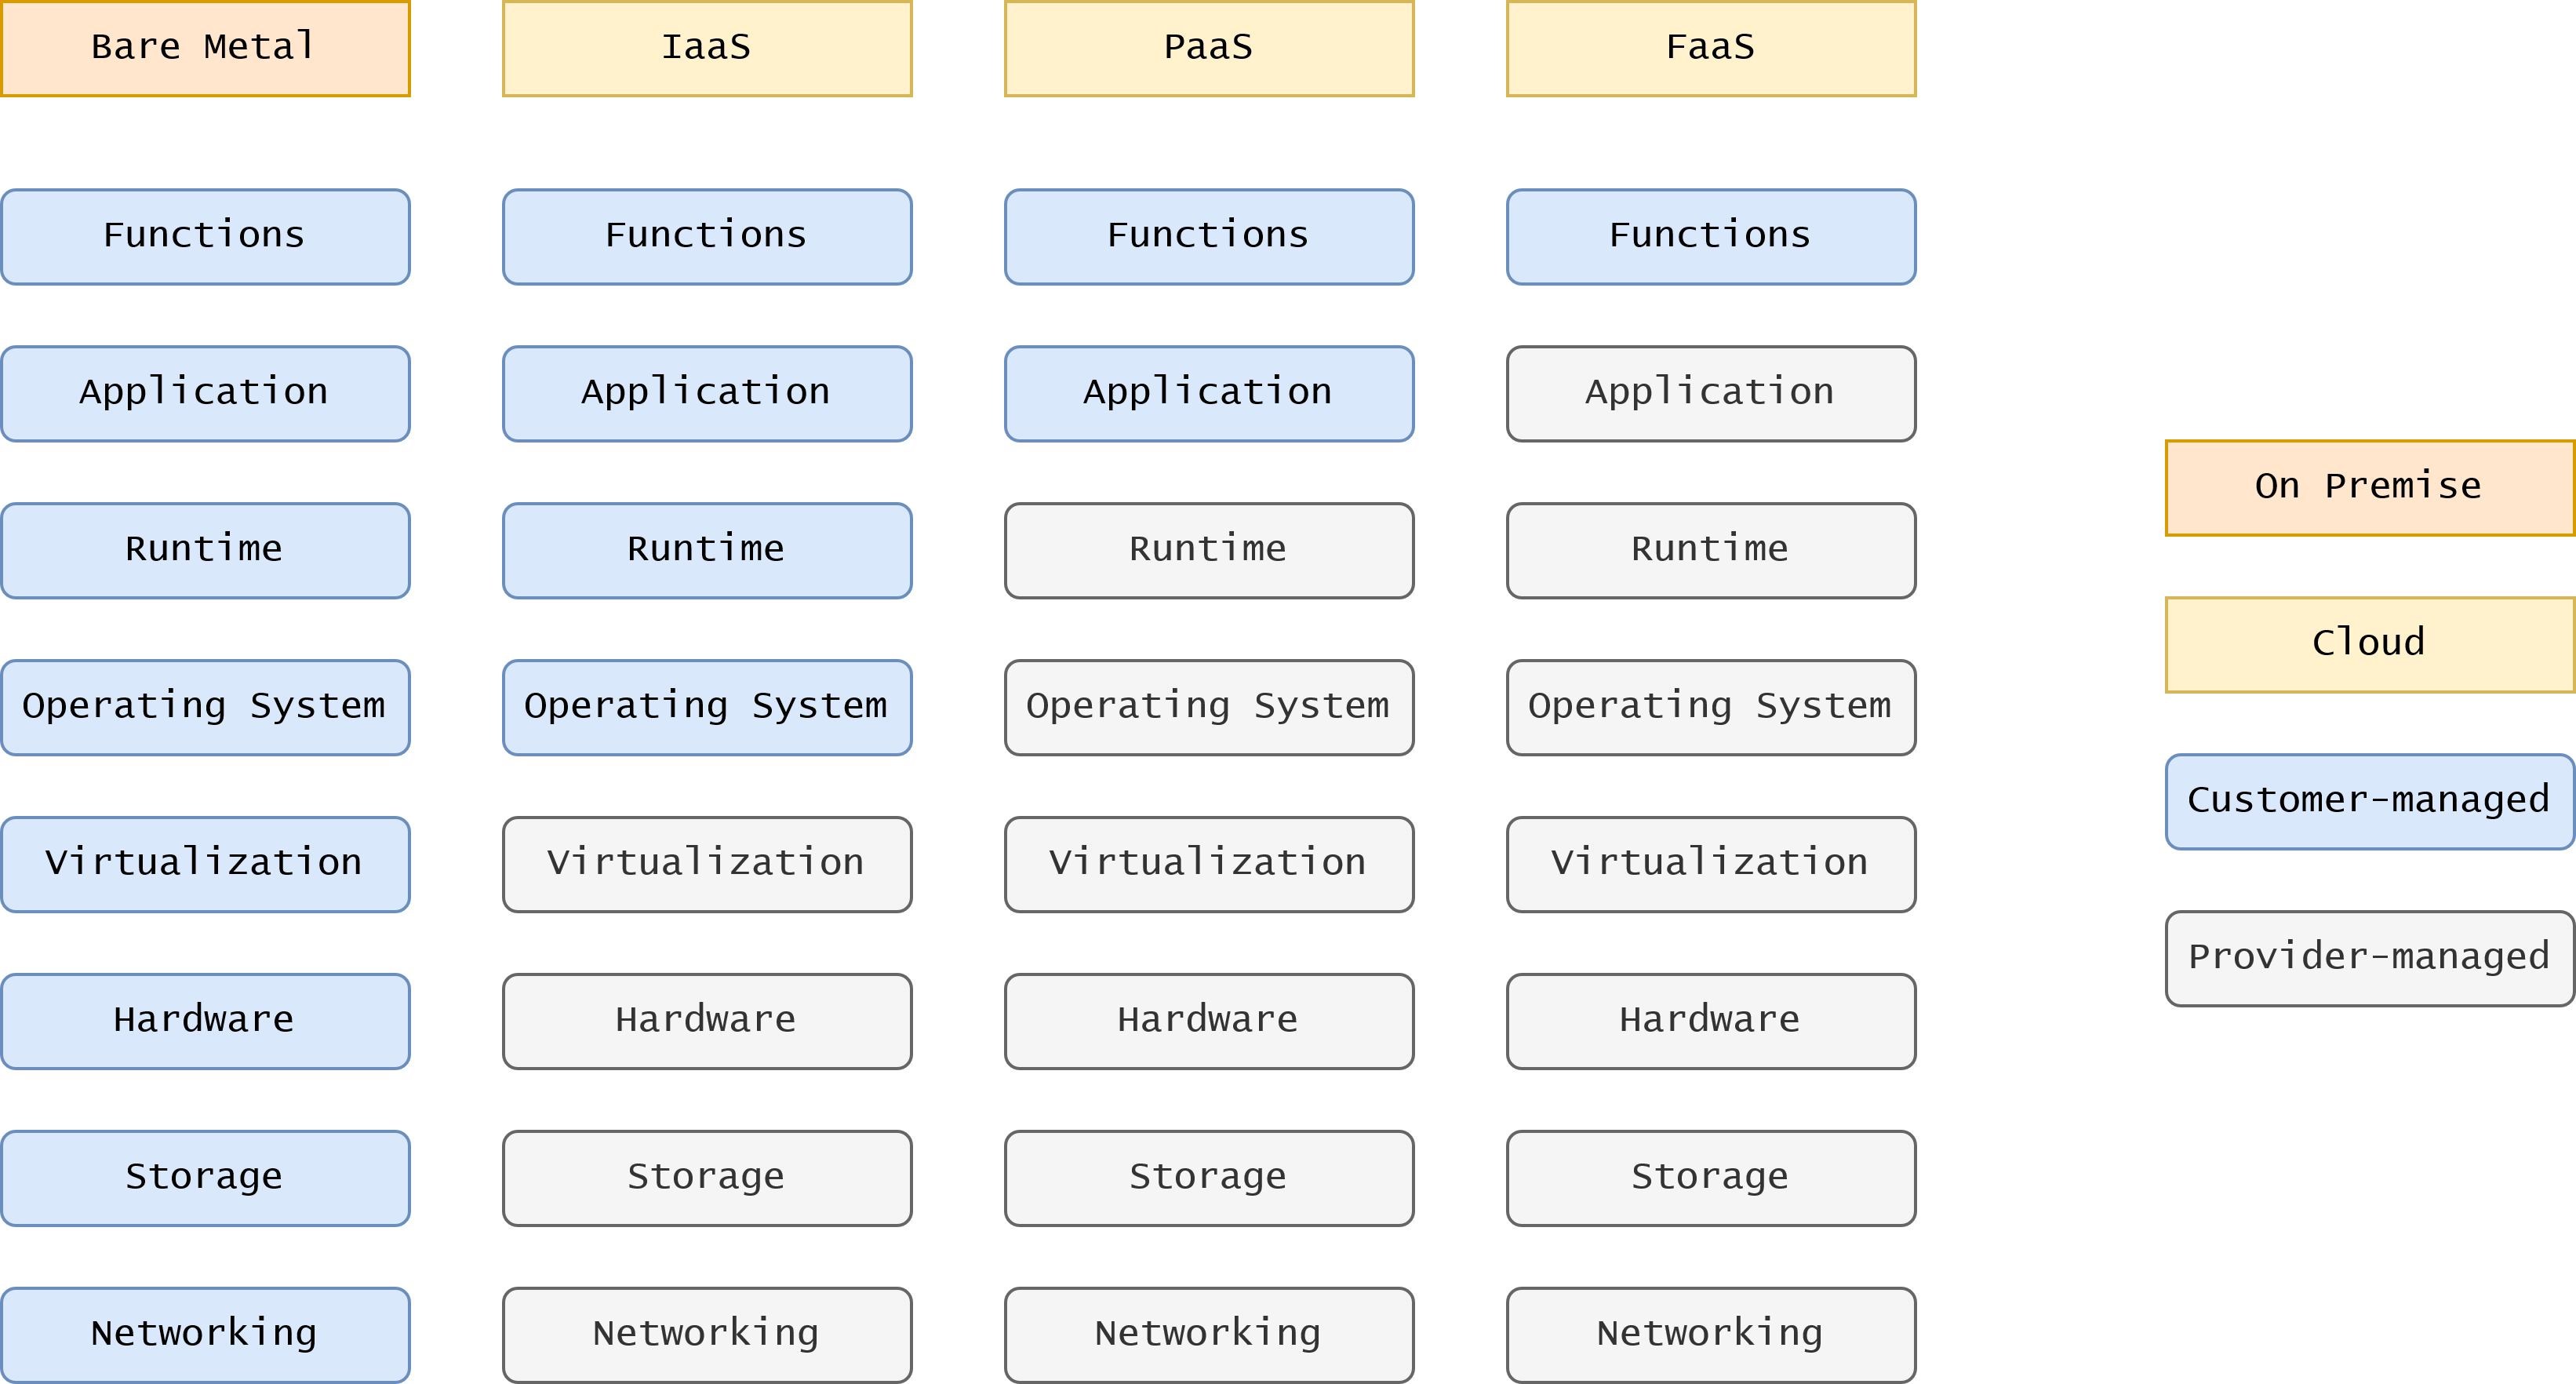
\includegraphics[width=\textwidth]{3_Chapitre1/figures/service-models.png}
	\caption[Comparaison entre différents modèles de service pour le cloud en termes de responsabilités pour le client et le fournisseur de service.]{Comparaison entre différents modèles de service pour le cloud en termes de responsabilités pour le client et le fournisseur de service (inspiré de la documentation Red Hat \protect \footnotemark).}
	\label{fig:service-model}
\end{figure}

\footnotetext{\url{https://www.redhat.com/en/topics/cloud-computing/iaas-vs-paas-vs-saas}}

Le NIST donne une définition formelle du cloud~\cite{mellNISTDefinitionCloud} en listant les caractéristiques essentielles d'une telle plateforme :

\begin{itemize}
    \item \textbf{Service à la demande} -- Les clients réservent des ressources matérielles de manière autonome, par exemple au travers d'une interface web, sans interagir avec un opérateur. En retour, ils n'ont généralement pas de contrôle fin sur la localité précise des ressources réservées ;
    \item \textbf{Accessible par le réseau} -- Ces ressources sont immédiatement mises à disposition des clients et accessibles par Internet ;
    \item \textbf{Partage des ressources} -- La puissance de calcul, les capacités de stockage et la bande passante sont partagées entre les clients du fournisseur de services. Des techniques de virtualisation sont mises en œuvre pour isoler les tâches déployées ;
    \item \textbf{Élasticité rapide} -- Les clients peuvent à tout moment décider d'augmenter ou de diminuer la quantité et les caractéristiques des ressources qu'ils réservent, de manière à garantir les performances de leurs applications ou maîtriser leurs coûts ;
    \item \textbf{Service mesuré} -- Les infrastructures cloud sont instrumentées de manière à fournir aux clients une information précise sur leur consommation de ressources, et les coûts monétaires associés.
\end{itemize}

\subsection{Modèles de service}

Ces caractéristiques sont déclinées dans trois modèles de service :

\begin{itemize}
    \item \textbf{Software as a Service} (SaaS) -- Cible l'utilisateur final en offrant l'accès à une application entièrement administrée par le fournisseur de services ;
    \item \textbf{Platform as a Service} (PaaS) -- Cible les clients qui souhaitent déployer leurs applications sans avoir la responsabilité d'administration des serveurs ;
    \item \textbf{Infrastructure as a Service} (IaaS) -- Cible les clients qui souhaitent un contrôle à grain fin sur leurs infrastructures. Les clients d'une offre IaaS sont responsables de l'administration de leurs serveurs, souvent virtuels. 
\end{itemize}

\subsection{Modèles de déploiement}

Enfin, ...

\begin{itemize}
    \item \textbf{Cloud privé} -- L'infrastructure est dédiée à une organisation qui regroupe plusieurs utilisateurs finaux. Ce modèle de déploiement est privilégié pour la sécurité et la confidentialité des données ;
    \item \textbf{Cloud public} -- L'infrastructure est partagée entre de nombreux clients hétérogènes, professionnels comme particuliers ;
    \item \textbf{Cloud communautaire} -- L'infrastructure est partagée entre différents acteurs ayant souvent des problématiques métier similaires (secteurs bancaire ou hospitalier par exemple) ;
    \item \textbf{Cloud hybride} -- Solution de répartition des tâches entre cloud privé et cloud public, en fonction de leur niveau de criticité.
\end{itemize}

\subsection{Qualité de service dans le cloud}

Problème : overbooking, overcommitting... conso d'énergie...

\section{Virtualisation}

\subsection{Multi-tenancy}

\subsection{Machines virtuelles}

\subsection{Conteneurs}

\section{Du monolithe aux micro-services}

\subsection{Passage à l'échelle dans le cloud}

\subsection{Développement cloud-native}

\section{Conclusion}


\clearemptydoublepage
\chapter{Serverless, allocation et placement dynamiques dans le cloud : État de l'art}

\section{Serverless}

Le modèle serverless constitue un changement de paradigme dans le cloud public : par opposition aux modèles traditionnels, les clients serverless ne réservent pas de ressources matérielles. L'exécution de leur code est dirigée par des événements (requêtes HTTP, tâches programmées, etc.) et la facturation s'effectue sur la base de l'usage réel des ressources. En contrepartie, la responsabilité de l'allocation des ressources et du placement des tâches incombe au fournisseur.

\subsection{Allocation des ressources}

\subsection{Placement des requêtes}

\section{Conclusion}

En libérant les utilisateurs de la contrainte du dimensionnement de leur infrastructure, le modèle de service serverless pour le cloud promet de faciliter le passage à l'échelle des applications. Grâce au mécanisme d'allocation à la demande, les clients peuvent bénéficier d'économies considérables, en ne payant plus pour des ressources qui seraient essentiellement dormantes, en attente d'une requête.

Toutefois, les solutions serverless actuelles présentent des inconvénients non négligeables qui limitent l'utilisation du serverless à des cas d'usage spécifiques. Ce paradigme se réalise aujourd'hui sous la forme d'un contrat sur le modèle de programmation : les utilisateurs des offres serverless doivent concevoir leurs applications comme un ensemble de fonctions pures -- idempotentes, leur exécution n'entraîne pas d'effets de bord -- ce qui constitue un lourd effort d'ingénierie.

Le fonctionnement de cette architecture logicielle, qui présente des similitudes avec l'architecture en micro-services, repose sur la communication par passage de messages entre fonctions. Les fonctions n'étant pas directement adressables sur le réseau dans les solutions commerciales actuelles, cette communication s'effectue par le biais d'un stockage lent : cela induit un surcoût important sur les performances de l'application lors des phases de composition et de synchronisation, jusqu'à parfois contrebalancer les gains offerts par le parallélisme massif inhérent au paradigme serverless.

Par ailleurs, le passage à l'échelle depuis zéro est associé à un fréquent risque de latence lors du réveil de l'application, puisque le fournisseur de services doit alors dynamiquement allouer des ressources matérielles et instancier l'environnement d'exécution des fonctions pour répondre à l'événement déclencheur. Les fournisseurs de services ont tendance à pré-allouer des ressources de manière à éviter ces démarrages à froid, ce qui contraint leurs gains potentiels en rendant ces ressources indisponibles pour d'autres clients.

Enfin, les accélérateurs matériels sont les grands absents de l'offre serverless commerciale. À l'heure où la demande en GPU et FPGA est croissante pour répondre aux besoins en calcul massivement parallèle, notamment dans le cadre de l'apprentissage machine ou de l'analyse de données "big data", les clients doivent se tourner vers une offre cloud plus conventionnelle s'ils souhaitent bénéficier de plateformes d'exécution hétérogènes.


\part{Contributions}

\clearemptydoublepage
\chapter{HeROfake : Orchestration serverless sur ressources hétérogènes pour le cloud privé}

\section{Introduction}
\label{section:herofake-introduction}

\begin{table*}[t]
    \centering
    \caption{State of the Art work on autoscaling platforms}
    \resizebox{\textwidth}{!}{
        \begin{tabular}{lccccccc}
            \toprule
            & Serverless & Target cloud platform     & SLA & Hardware heterogeneity & Resources usage & Energy consumption & Cost-aware \\
            \cmidrule(lr){2-2}\cmidrule(lr){3-3}\cmidrule(lr){4-4}\cmidrule(lr){5-5}\cmidrule(lr){6-6}\cmidrule(lr){7-7}\cmidrule(lr){8-8}
            Swayam~\cite{gujaratiSwayamDistributedAutoscaling2017}        & \xmark         & Private (Azure, in-house) & \cmark& \xmark                     & \cmark            & \xmark                 & \xmark         \\
            Pigeon~\cite{lingPigeonDynamicEfficient2019}                  & \cmark       & Private                   & \xmark  & \cmark                   & \cmark            & \xmark                 & \xmark         \\
            MArk~\cite{zhangMArkExploitingCloud}                          & \xmark         & Public (AWS)              & \cmark& \cmark                   & \cmark            & \xmark                 & \cmark       \\
            ENSURE~\cite{sureshENSUREEfficientScheduling2020}             & \cmark       & Private                   & \xmark  & \xmark                     & \cmark            & \xmark                 & \cmark       \\
            Mampage et al.~\cite{mampageDeadlineawareDynamicResource2021} & \cmark       & Private                   & \cmark& \xmark                     & \cmark            & \xmark                 & \cmark       \\
            Atoll~\cite{singhviAtollScalableLowLatency2021}               & \cmark       & Private                   & \cmark& \xmark                     & \xmark              & \xmark                 & \xmark         \\
            INFless~\cite{yangINFlessNativeServerless2022}                & \cmark       & Private                   & \cmark& \xmark                     & \cmark            & \xmark                 & \cmark       \\
            SMIF~\cite{choSLADrivenMLInference}                           & \cmark       & Private                   & \cmark& \cmark                   & \cmark            & \xmark                 & \xmark         \\
            Target solution                                                & \cmark       & Private                   & \cmark& \cmark                   & \cmark            & \cmark               & \cmark       \\ \bottomrule
        \end{tabular}
    }
    \label{table:herofake-sota}
\end{table*}

\textbf{Modèle serverless}. Le serverless peut être compris à la fois comme un modèle de programmation, appelé Function as a Service (FaaS), et comme un modèle de déploiement pour le cloud. Dans un tel modèle, les développeurs conçoivent leurs applications comme une composition de fonctions sans état dont l'exécution est pilotée par des événements~\cite{SchleierSmith2021WhatSC}. 
Les services serverless libèrent les locataires d'une réservation complexe des ressources, car ils sont conçus pour gérer les exigences de mise à l'échelle à la demande.

Dans le modèle FaaS, les fournisseurs ne facturent les clients qu'en fonction de leur utilisation réelle des ressources~\cite{jonasCloudProgrammingSimplified2019}. Ils sont entièrement responsables du déploiement d'une gestion intelligente des ressources et du multiplexage à une granularité plus fine afin d'optimiser les mesures de qualité de service (QoS) telles que le temps de réponse, la consommation d'énergie, etc.

\textbf{Détection de deepfake et serverless}. Le travail présenté dans cet article faisait partie d'un projet (à l'institut de recherche b{\textless\textgreater}com \footnote{\href{https://b-com.com/en}{https://b-com.com/en}}) visant à déployer un service de détection de deepfake économe en énergie dans un cloud hétérogène. Les deepfakes sont des images, des vidéos ou des discours synthétiques, créés numériquement pour imiter une personne existante de manière à tromper les spectateurs. La détection de deepfake consiste à entraîner un réseau neuronal convolutif (CNN) pour détecter des modèles d'incohérences introduits dans le processus de création.

Les fonctions utilisées par notre application deepfake répondent à trois caractéristiques principales pour des charges de travail serverless adaptées~\cite{cncf2018whitepaper} : leur exécution peut être rendue parallèle (plusieurs images indépendantes), elles sont stateless (pure transformation sur les données d'entrée) et event-driven (lancées après l'upload des données).

D'une part, la détection de deepfake à l'aide de réseaux de neurones convolutifs (CNN) est une tâche qui peut tirer parti de la concurrence en exécutant plusieurs convolutions en parallèle et/ou en traitant différentes images sur plusieurs threads. Ces tâches sont essentiellement sans état, car elles appliquent une transformation pure sur les données d'entrée - en prenant une image en entrée et en renvoyant une valeur booléenne en sortie. Une telle application est pilotée par les événements, le calcul commençant après le téléchargement d'une image d'entrée. Ce sont là trois caractéristiques principales des charges de travail serverless appropriées~\cite{cncf2018whitepaper}.

D'autre part, les ressources matérielles nécessaires pour exécuter cette application à l'échelle seraient nombreuses et coûteuses : être en mesure de faire évoluer dynamiquement les ressources en fonction de la demande permettrait au client de réaliser d'importantes économies et au fournisseur d'accepter plus de clients sur le même nombre de nœuds.

Par conséquent, nous soutenons que le modèle de service serverless est parfaitement adapté à l'inférence à la demande rentable utilisant des CNN.

\textbf{Hétérogénéité matérielle dans le cloud}. Les infrastructures cloud sont de plus en plus hétérogènes pour répondre aux besoins des applications à forte intensité de données telles que l'apprentissage automatique de modèles ou l'analyse de données massives~\cite{reissHeterogeneityDynamicityClouds}. Cependant, les processeurs spécialisés et les GPU doivent encore être mis à la disposition des clients dans les offres serverless~\cite{khandelwalTaureauDeconstructingServerless2020}. L'accélération matérielle devrait être décidée par le fournisseur sur la base d'une application ou d'une demande.

Les travaux de l'état de l'art montrent que l'utilisation de ce matériel dans un cadre cloud permet des gains substantiels en termes de temps d'exécution et de consommation d'énergie~\cite{10.1145/3369583.3392679, 9195730}. Cependant, les orchestrateurs de référence tels que Kubernetes avec Knative ou OpenWhisk ne prennent pas en charge l'allocation dynamique de ce type de matériel.

\textbf{Défi de performance pour le déploiement serverless}. En raison de la nature transitoire des ressources FaaS non réservées, la latence, le débit et la continuité du service sont difficiles à garantir~\cite{vaneykSPECRGCloud2018, dartoisCuckooOpportunisticMapReduce2019}. Lorsque les applications ne reçoivent pas de demandes entrantes, les bacs à sable des fonctions sont détruits au lieu d'être maintenus dans un état d'inactivité. Ensuite, lorsqu'une nouvelle demande arrive, le fournisseur doit (ré)allouer des ressources et initialiser des fonctions pour déployer de nouveaux bacs à sable : c'est ce qu'on appelle un démarrage à froid. Les temps de démarrage à froid sont très pénalisants pour les performances de l'application, ils peuvent même dominer les temps d'exécution totaux~\cite{mullerLambadaInteractiveData2020}.

De plus, dans les offres commerciales serverless actuelles, les accords de niveau de service (SLA) sont généralement limités à des tentatives automatisées (redémarrages) en cas d'échec, et les fournisseurs de FaaS limitent généralement le temps d'exécution des fonctions serverless à quelques minutes. L'absence de garanties de qualité de service dans les offres commerciales serverless les empêche d'être plus largement utilisées~\cite{buyyaSLAorientedResourceProvisioning2011}.

\textbf{Énoncé du problème -- mettre tout ensemble}. Le problème que nous tentons de résoudre dans cet article est de déterminer comment dimensionner automatiquement et de manière réactive des ressources matérielles hétérogènes dans le cloud en fonction de la charge sur l'application et des exigences de qualité de service des utilisateurs, tout en maintenant le coût des ressources et de l'énergie au niveau le plus bas possible pour le fournisseur. Nous considérons une application de détection de deepfake comme cas d'étude pour² notre travail.

\textbf{État de l'art}. Des études antérieures ont exploré le besoin d'une plateforme de mise à l'échelle automatique qui prend en charge les tâches de courte durée comprises dans des applications telles que l'apprentissage automatique en tant que service. Le tableau~\ref{table:herofake-sota} résume les différences entre ces solutions et la plateforme cible que nous essayons d'atteindre, et la section~\ref{section:herofake-sota} fournit des détails supplémentaires. Bien que de nombreuses études aient établi la nécessité d'une accélération à la demande comme solution pour garantir le temps de réponse des fonctions, aucune n'a mesuré l'impact de l'exploitation des ressources hétérogènes sur la consommation d'énergie dynamique. En outre, les études précédentes considèrent la consolidation des tâches comme un moyen de libérer des ressources pour d'autres calculs - nous soutenons que ces techniques ouvrent des possibilités pour le fournisseur de services d'appliquer des politiques d'économie d'énergie dans le cloud privé. Enfin, comme les plateformes serverless sont à usage général et conçues pour être hautement configurables, notre solution cible devrait être consciente des coûts pour permettre au fournisseur de faire des choix de configuration se rapportant à leurs propres objectifs.

\textbf{Notre contribution}. Nous soutenons que l'utilisation opportuniste des accélérateurs matériels (GPU et FPGA) pour planifier les tâches de détection de deepfake peut permettre aux fournisseurs de cloud de garantir le temps de réponse des tâches serverless et d'atteindre le SLA tout en réduisant l'utilisation des ressources et la consommation d'énergie.

Dans cet article, nous proposons un cadre complet pour déployer une application de détection de deepfake sur un cloud serverless. Ce cadre comprend une phase hors-ligne et une phase en ligne. Le \textbf{phase hors-ligne} est utilisé pour caractériser la performance et le comportement énergétique des plates-formes matérielles hétérogènes déployées. La \textbf{phase en ligne} consiste en une plateforme de mise à l'échelle automatique et une stratégie d'ordonnancement qui utilisent efficacement les ressources matérielles hétérogènes (caractérisées) pour atteindre les accords de niveau de service par demande tout en réduisant la consommation d'énergie de la plateforme. 

Pour cette étude de cas, nous avons conçu un environnement de simulation qui modélise l'infrastructure d'une application de détection de deepfake, exécutée par le fournisseur en tant que Software as a Service à l'aide d'une infrastructure serverless.

\textbf{Certains chiffres de performance}. Avec notre politique d'allocation et d'ordonnancement, nous avons été en mesure de traiter 50000 tâches dans le même makespan que Knative avec moins de 36\% de pénalités de QoS. Notre cadre réduit la consommation d'énergie pour l'exécution des tâches de près de 35\% et permet au fournisseur de réduire davantage la consommation d'énergie statique en consolidant les tâches sur moins de 29\% des nœuds disponibles.

Le document est organisé comme suit : dans une première section, nous décrivons le modèle de plateforme global pour le projet. Ensuite, nous décrivons la plateforme d'exécution et la phase de caractérisation de la charge de travail. Dans la section III, nous décrivons les défis de l'orchestration de ressources serverless, notre modèle de tâches et les politiques d'allocation et d'ordonnancement de l'orchestrateur. La section IV présente notre méthodologie d'évaluation et une discussion des résultats expérimentaux. La section V donne des détails concernant l'état de l'art sur les plateformes d'autoscaling. Enfin, nous concluons par quelques perspectives pour les travaux futurs.

\section{Déployer des tâches de détection de deepfake dans un cloud serverless}
\label{section:herofake-deepfake}

\begin{figure*}[t]
\centering
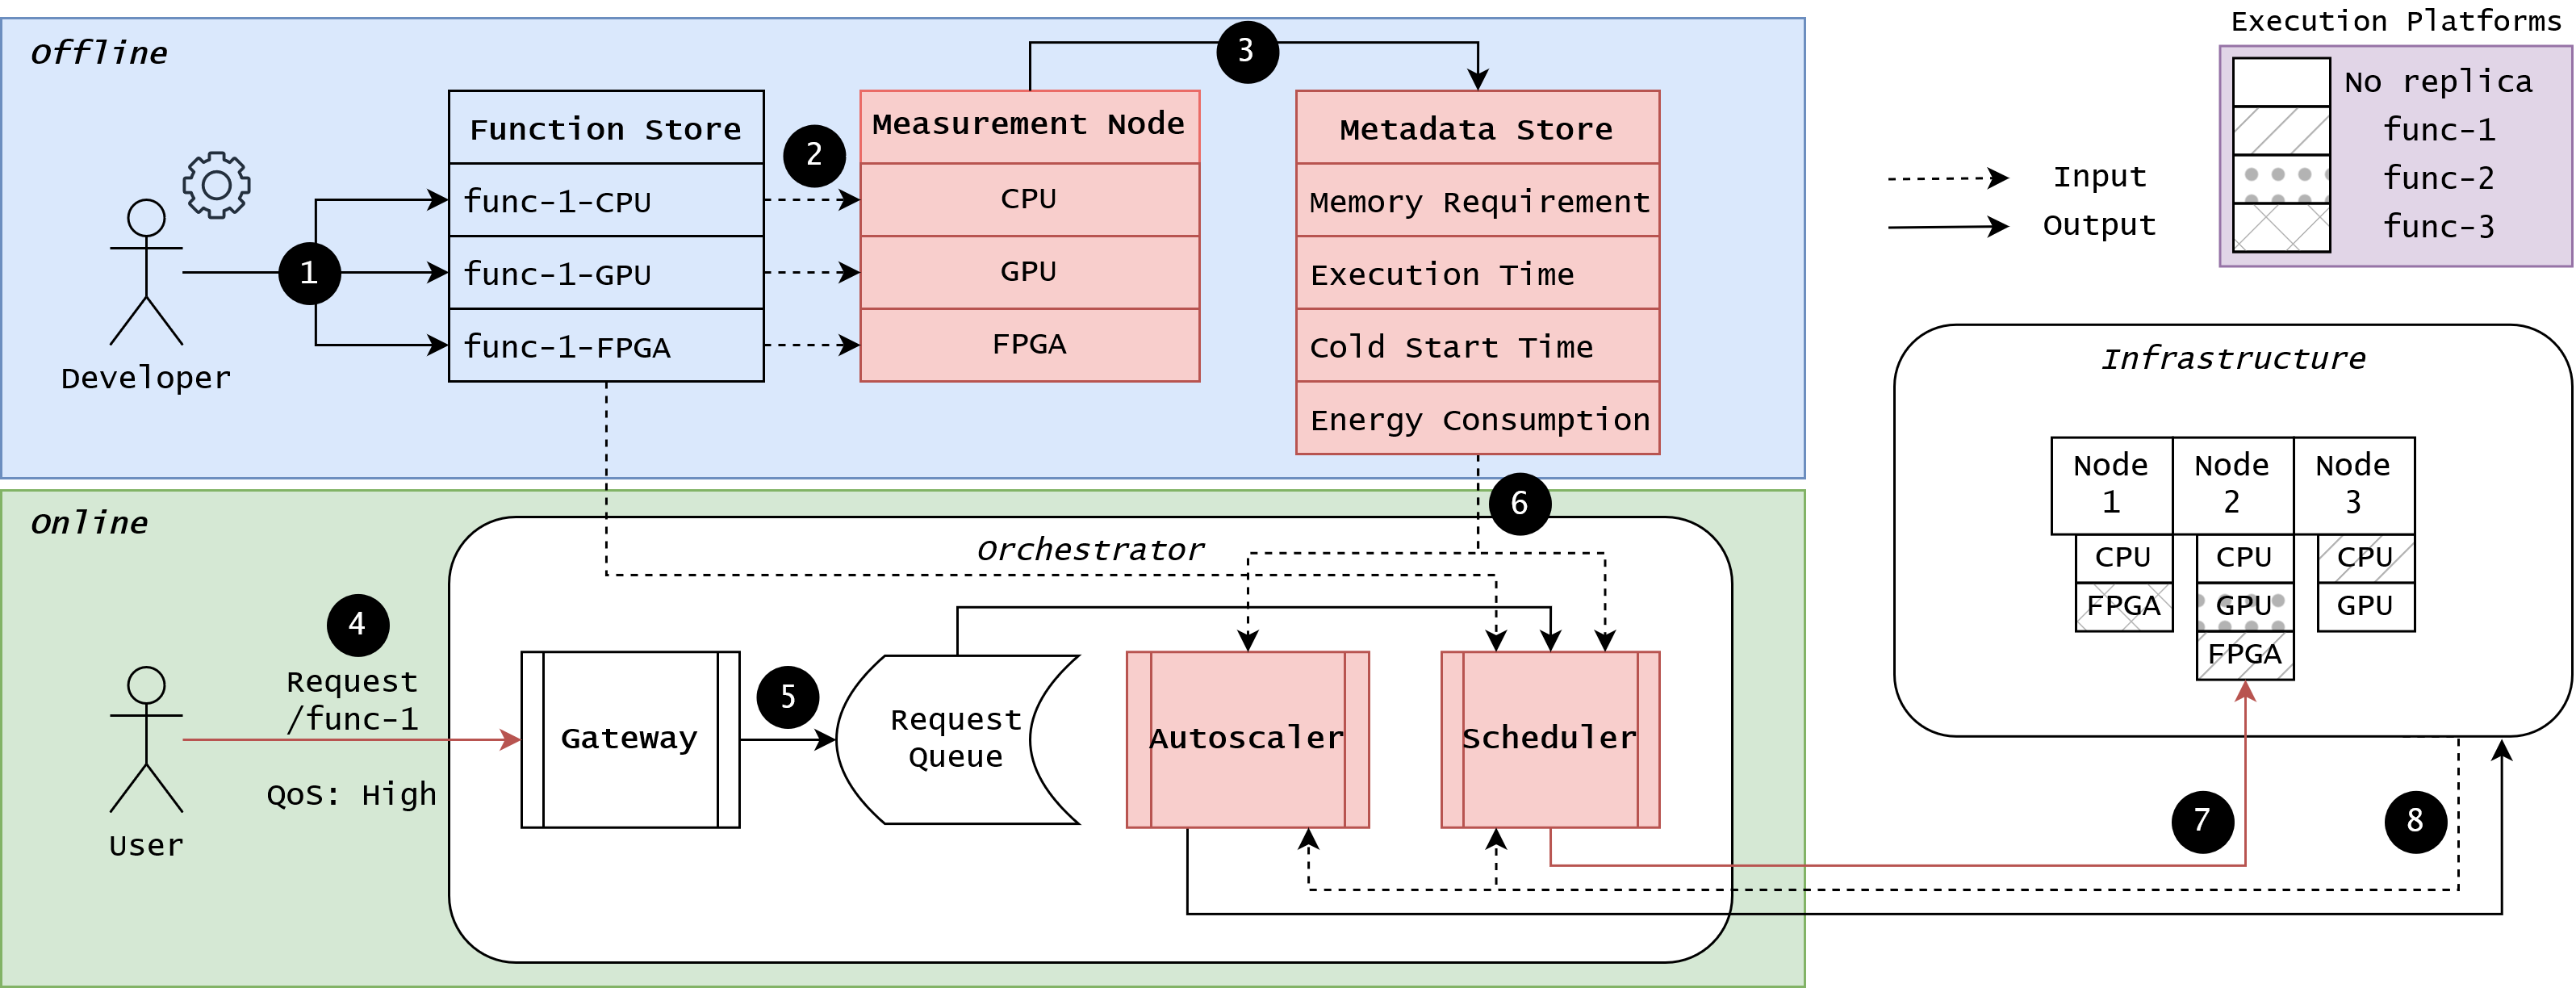
\includegraphics[width=0.8\textwidth]{5_Chapitre3/figures/placement.png}
\caption{Plateforme de détection de deepfake serverless, vue d'ensemble du système.}
\label{figure:herofake-placement}
\end{figure*}

Cette section présente le modèle de plateforme serverless utilisé et le projet global.

\subsection{Modèle de la plateforme}

Nous considérons un système de détection de deepfake qui est déployé comme une application serverless composée de trois fonctions sans état qui réalisent des tâches d'inférence sur des images d'entrée. Ces images sont toutes RVB et de taille $224 * 224$ pixels~\footnote{Notez que les vidéos ne sont pas encore prises en compte dans notre projet.}.

La figure~\ref{figure:herofake-placement} présente la plateforme utilisée, nous distinguons une phase \textit{hors-ligne} (boîte bleue dans la figure) et une phase \textit{en ligne} (boîte verte dans la figure). Pendant la phase hors-ligne, nous collectons les métadonnées relatives à l'exécution des tâches sur les accélérateurs hétérogènes ; pendant la phase en ligne, nous allouons les ressources et programmons les tâches.

Les demandes d'invocation de fonctions émanant des utilisateurs sont reçues par le fournisseur et traitées par l'orchestrateur. Dans notre modèle, une invocation de fonction correspond à un \textit{tâche}. L'utilisateur sélectionne l'un des trois modèles fournis (ResNet50, VGG16 et VGG19, voir Section~\ref{section:herofake-offline:workload}) et l'utilise pour détecter un éventuel deepfake sur une image.

L'infrastructure du fournisseur de cloud est modélisée comme un ensemble de \textit{nœuds} hétérogènes (Section~\ref{model:nodes}) comprenant diverses combinaisons de \textit{plateformes} (Section~\ref{model:platforms}) qui peuvent exécuter des \textit{tâches} entrantes (Section~\ref{model:tasks}). 

\subsubsection{Nœuds}
\label{model:nodes}
Un nœud est un serveur disponible dans l'infrastructure du fournisseur de services. Dans ce travail, nous ne tenons pas compte de la localité du stockage et des données. Les données d'entrée sont toujours fournies \textit{via} le téléchargement de fichiers par l'utilisateur au moment de sa demande.
Ainsi, la seule caractéristique qui définit un nœud dans notre modèle d'infrastructure est la taille de la mémoire dédiée. Un nœud est constitué d'un ensemble de plateformes d'exécution définies ci-après.

\subsubsection{Plateformes d'exécution}
\label{model:platforms}

Une plateforme d'exécution est une unité de traitement matérielle disponible sur un nœud. Chaque plateforme consomme une quantité d'énergie à l'état "inactif" exprimée en kilowattheures (kWh). Lorsqu'elle commence à exécuter une tâche, elle consomme une énergie supplémentaire caractérisée par les propriétés/le type de la tâche : elle est alors dans un état "actif". Nous distinguons le temps "inactif" et le temps "actif" pour chaque plateforme, afin de mesurer l'utilisation des ressources.
Les plateformes sont caractérisées par un \textit{type de plateforme} qui englobe les paramètres suivants :

\begin{itemize}
    \item \textit{Type de matériel} -- CPU, GPU ou FPGA ;
    \item \textit{Prix} -- le coût d'acquisition d'une telle plateforme par le fournisseur de services cloud ;
    \item \textit{Énergie au repos} -- la consommation d'énergie de base de la plateforme lorsqu'elle n'exécute aucune tâche.
\end{itemize}

\textbf{Mise en cache des tâches et modèle de démarrage à froid}. Nous considérons un mécanisme simple de mise en cache des tâches au niveau de la plateforme, qui s'apparente à un mécanisme de maintien en vie~\cite{7279063}. Dans notre système, si une plateforme a déjà exécuté une tâche de type $t$ et qu'une nouvelle tâche du même type $t$ est programmée sur cette même plateforme, le délai de démarrage à froid n'est pas appliqué. Toutefois, si cette même plateforme devait exécuter une tâche de type différent $tt$, la tâche subira un démarrage à froid avant d'entrer dans sa phase d'exécution. Enfin, si la plateforme n'a pas été allouée précédemment, la tâche subira également un délai de démarrage à froid.

\subsection{Description générale du système}

L'institut de recherche b{\textless\textgreater}com travaille sur un projet qui vise à déployer une application de détection de deepfake sur un cloud privé. Les utilisateurs soumettent une image au système et lorsque leur demande est satisfaite, ils obtiennent une valeur booléenne en guise de réponse. L'application vise différentes catégories d'utilisateurs : certains d'entre eux peuvent être des médias ou des autorités ayant des exigences élevées en matière de qualité de service, tandis que d'autres peuvent être des utilisateurs occasionnels tolérant une latence plus élevée.

Pour différencier ces catégories d'utilisateurs, nous proposons différents niveaux d'accords de niveau de service par demande. Les utilisateurs ayant des exigences plus élevées accepteront de payer un prix plus élevé par demande, mais si nous ne parvenons pas à satisfaire leur demande dans le temps de réponse imparti, nous consentirons à une remise - plus le niveau de qualité de service est élevé, plus la remise est importante. Le fournisseur est donc fortement incité, sur le plan pécuniaire, à assurer la qualité de service.

\textbf{Phase hors-ligne}. Dans notre plateforme, le cycle de vie de l'application commence par une phase hors-ligne au cours de laquelle le développeur fournit le code de ses fonctions pour différentes architectures matérielles \Circled{1}. Ce code est stocké dans un référentiel de fonctions. Les fonctions sont ensuite déployées sur un nœud de mesure \Circled{2} où elles sont exécutées afin de générer des métadonnées relatives aux fonctions : les besoins en mémoire, le temps d'exécution, le temps de démarrage à froid et la consommation d'énergie pour chaque fonction sont écrits dans un magasin de métadonnées \Circled{3}. La phase hors-ligne doit être exécutée une fois pour une fonction donnée sur une plateforme donnée, elle est décrite dans la section~\ref{section:herofake-offline}.

\textbf{Phase en ligne}. Lorsqu'un utilisateur envoie une demande à l'application \Circled{4}, il fournit une image d'entrée et spécifie le niveau de qualité de service souhaité. La demande est ajoutée à une file d'attente \Circled{5} au niveau de l'orchestrateur. Lorsque le planificateur extrait la demande de la file d'attente, le magasin de métadonnées est interrogé pour récupérer les métadonnées de fonction appropriées \Circled{6}.

L'ordonnanceur tente ensuite de planifier une tâche (c'est-à-dire l'invocation d'une fonction) pour répondre à la demande. Les tâches sont placées sur des \textit{répliques} de fonctions \Circled{7} déjà déployées. Ces répliques peuvent être des conteneurs ou des machines virtuelles, c'est-à-dire des environnements d'exécution dédiés pour la fonction donnée.
Simultanément, l'autoscaler surveille les files d'attente de requêtes dans toutes les répliques de fonctions \Circled{8}. Le rôle de l'autoscaler est de dimensionner l'allocation des ressources en fonction des fluctuations de charge pour chaque fonction.
L'ordonnanceur et l'autoscaler sont décrits dans la section~\ref{section:herofake-online}.

\section{Phase hors-ligne : mesures et extraction des métadonnées}
\label{section:herofake-offline}

\subsection{Caractérisation des plateformes d'exécution}

\begin{table}[t]
\caption{Execution platform characterization}
\begin{center}
\resizebox{\columnwidth}{!}{%
\begin{tabular}{|c|c|c|c|c|}
\hline
                             \textbf{Platform} & \textbf{Hardware type}& \textbf{Price (MSRP)} & \textbf{Idle energy} \\ \hline
Intel Xeon ES-1620 v4         & CPU           & 294          & 0.067       \\ \hline
Nvidia GeForce RTX 2070 Super & GPU           & 499          & 0.010       \\ \hline
Xilinx Alveo U250             & FPGA          & 7695         & 0.030       \\ \hline
\end{tabular}%
}
\end{center}
\label{table:herofake-platforms}
\end{table}

L'utilisation de l'inférence par apprentissage profond et les impacts énergétiques augmentant simultanément dans l'informatique, l'efficacité énergétique des dispositifs cibles devient une préoccupation majeure. Les cartes d'accélération basées sur les FPGA sont décrites comme un concurrent pertinent face à l'approche dominante des GPU. Notre étude propose un benchmark, utilisant des approches basées sur les réseaux neuronaux convolutifs (CNN) pour la détection de deepfake sur les technologies CPU, GPU et FPGA en ce qui concerne l'efficacité énergétique pendant le temps d'inférence. Notre comparaison porte sur la consommation d'énergie, la vitesse d'inférence et la précision en utilisant le traitement CPU et GPU traditionnel par rapport au FPGA. Ces mesures sont cruciales pour une orchestration efficace sur des plateformes hétérogènes.

Le CPU utilisé était un Intel Xeon CPU ES-1620 v4 (3,5 GHz) tandis que le GPU était un Nvidia GeForce RTX 2070 Super qui peut être utilisé avec les nouvelles versions des frameworks d'IA. Par conséquent, les deux étaient compatibles avec TensorFlow, c'est-à-dire la plateforme utilisée pour l'inférence. En ce qui concerne le FPGA, nous avons utilisé l'Alveo U250, une carte de cloud computing de Xilinx, qui est compatible avec Vitis-AI~\cite{vitis-ai}. Les processus de silicium utilisés pour les deux dispositifs sont similaires (12 nm pour le GPU et 16 nm pour le FPGA), mais le GPU peut obtenir un léger avantage dans ce benchmark grâce à sa technologie de silicium plus avancée.

Pour effectuer l'inférence sur le FPGA, nous avons utilisé Vitis-AI. Au moment de cette étude, la dernière version disponible (v. 2.0) a été utilisée. Vitis-AI propose deux méthodes pour l'optimisation des modèles. La première est l'élagage, qui consiste à réduire la complexité du modèle par une compression tout en supprimant certaines sections non critiques de l'arbre. La seconde est la quantification, où l'on convertit les poids flottants de 32 bits en entiers de 8 bits. Cette dernière méthode, qui est librement disponible, est celle que nous avons utilisée pour optimiser notre modèle avant la compilation, qui convertit notre modèle en instructions DPU (Deep Learning Processing Unit).

\subsection{Caractérisation des tâches logicielles}
\label{section:herofake-offline:workload}

\begin{table}[t]
\caption{Workload characterization }
\centering
\resizebox{\columnwidth}{!}{%
\begin{tabular}{|c|cc|ccc|ccc|ccc|}
\hline
Task     & \multicolumn{2}{c|}{Memory (GB)} & \multicolumn{3}{c|}{Cold start (s)}                              & \multicolumn{3}{c|}{Execution time (s)}                         & \multicolumn{3}{c|}{Energy (mWh)}                            \\ \hline
         & \multicolumn{1}{c|}{CPU}  & GPU  & \multicolumn{1}{c|}{CPU}   & \multicolumn{1}{c|}{GPU}   & FPGA   & \multicolumn{1}{c|}{CPU}   & \multicolumn{1}{c|}{GPU}   & FPGA  & \multicolumn{1}{c|}{CPU}  & \multicolumn{1}{c|}{GPU}  & FPGA \\ \hline
ResNet50 & \multicolumn{1}{c|}{1.3}  & 3.3  & \multicolumn{1}{c|}{1.232} & \multicolumn{1}{c|}{2.340} & 9.952  & \multicolumn{1}{c|}{0.124} & \multicolumn{1}{c|}{0.024} & 0.009 & \multicolumn{1}{c|}{3.11} & \multicolumn{1}{c|}{1.7}  & 0.5  \\ \hline
VGG16    & \multicolumn{1}{c|}{1.8}  & 3.3  & \multicolumn{1}{c|}{2.514} & \multicolumn{1}{c|}{4.641} & 14.528 & \multicolumn{1}{c|}{0.143} & \multicolumn{1}{c|}{0.046} & 0.010 & \multicolumn{1}{c|}{4.34} & \multicolumn{1}{c|}{3.43} & 0.55 \\ \hline
VGG19    & \multicolumn{1}{c|}{1.9}  & 3.4  & \multicolumn{1}{c|}{2.559} & \multicolumn{1}{c|}{4.641} & 14.758 & \multicolumn{1}{c|}{0.167} & \multicolumn{1}{c|}{0.048} & 0.012 & \multicolumn{1}{c|}{5.16} & \multicolumn{1}{c|}{3.58} & 0.65 \\ \hline
\end{tabular}
}%
\label{table:herofake-tasks}
\end{table}

Pour les besoins de cette étude, trois modèles populaires ont été formés. Le premier est basé sur les réseaux résiduels (ResNet50), qui utilise des blocs résiduels et peut être entraîné efficacement~\cite{NEURIPS2019_7716d0fc}. Le deuxième est VGG16 (VGG pour Visual Geometry Group), qui utilise uniquement des convolutions comme blocs~\cite{DBLP:journals/corr/SimonyanZ14a} et le troisième est VGG19, une variante de VGG16 avec trois couches supplémentaires~\cite{biom10070984}. Ces réseaux sont entraînés sur un GPU, l'entraînement n'étant pas le sujet de cette étude.

\subsection{Mesures de performances}

\begin{figure}[t]
\centering
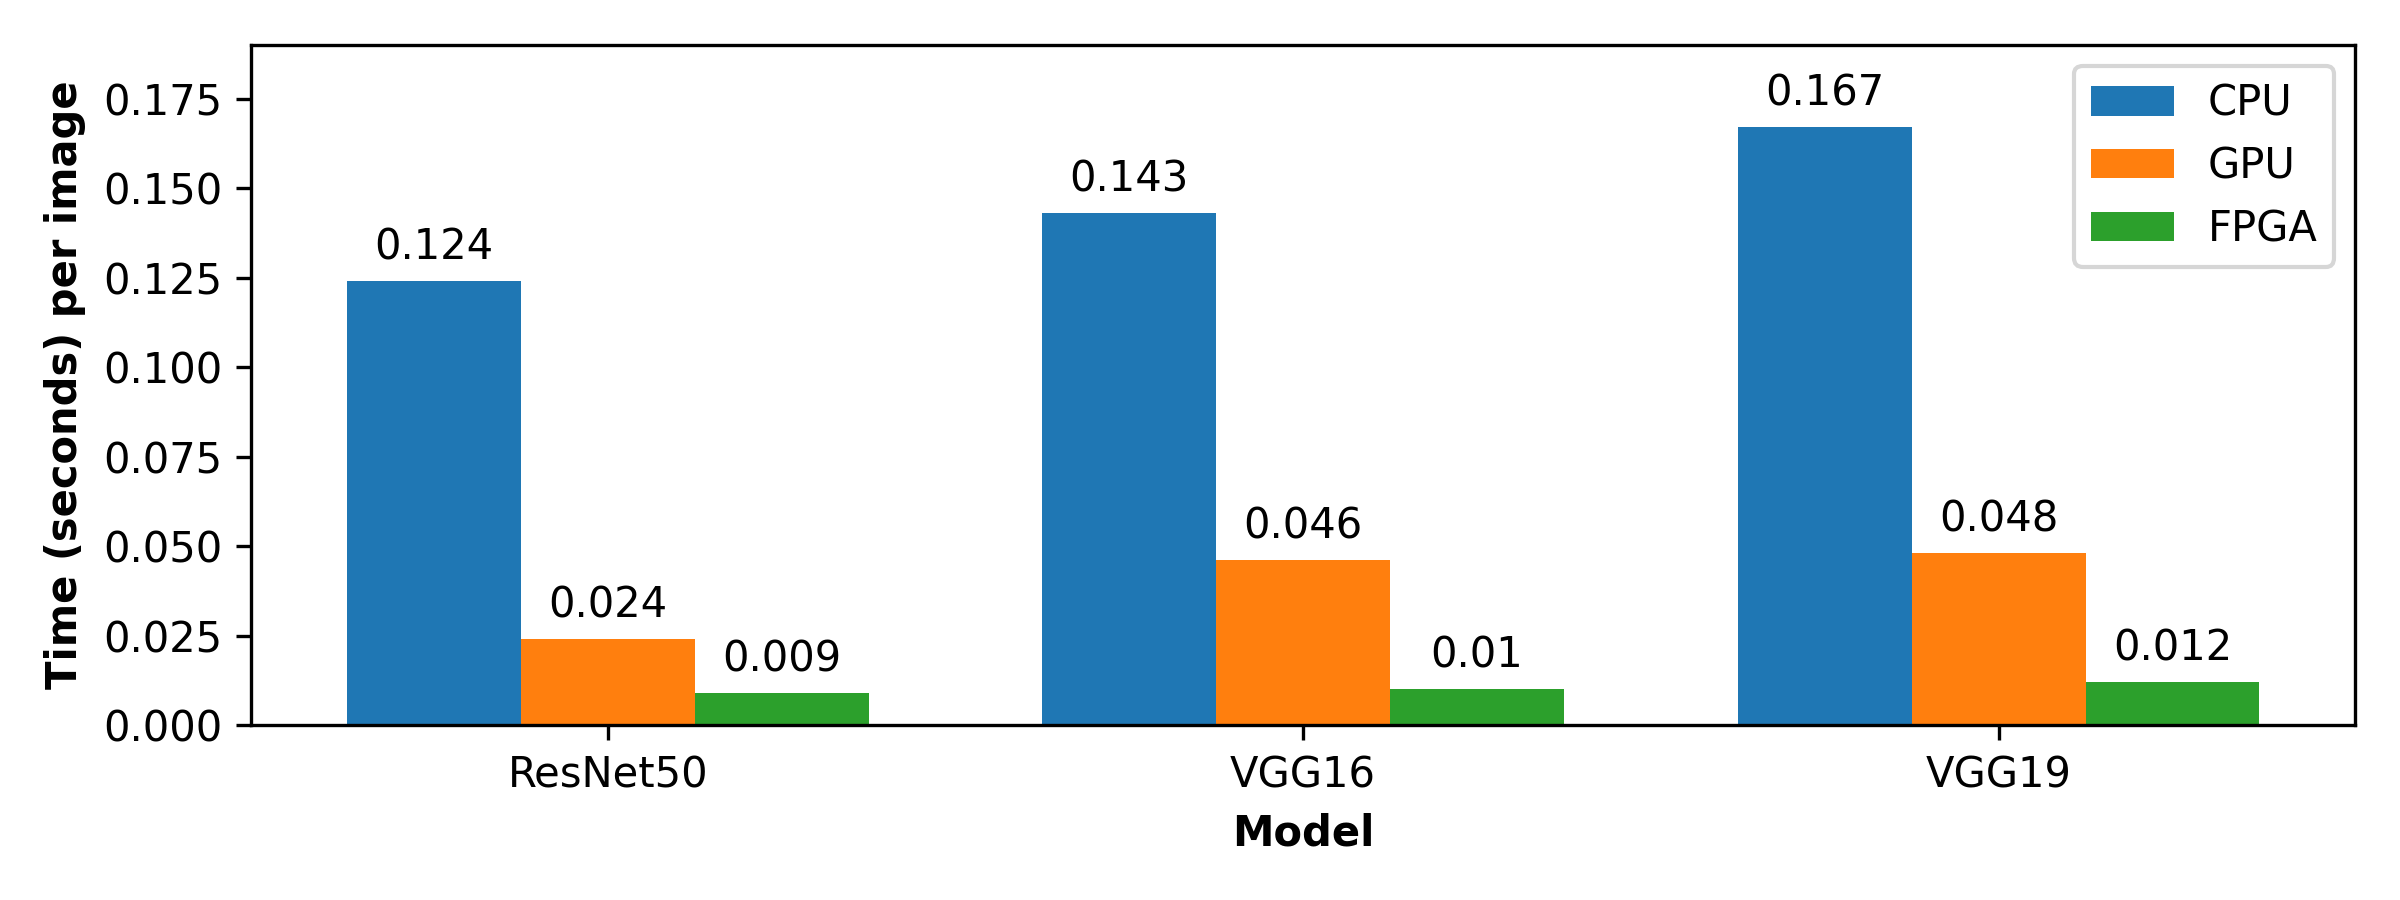
\includegraphics[width=\columnwidth]{5_Chapitre3/figures/characterization/time_of_inference_1_image.png}
\caption{Inference time for one image with ResNet50, VGG16 and VGG19.}
\label{figure:herofake-time-inference}
\end{figure}

La carte d'accélération FPGA étant censée être plus efficace qu'un CPU ou un GPU~\cite{5272532}, la comparaison du temps d'inférence avec ces trois technologies est une première condition pour permettre la comparaison du coût énergétique par image. L'évaluation des performances en termes de temps d'exécution a été réalisée avec les mêmes 10 000 images pour les trois modèles différents. Nous avons construit un ensemble de données deepfake à deux classes, les vraies provenant de l'ensemble de données CelebA~\cite{https://doi.org/10.48550/arxiv.1411.7766}, et les fausses générées à l'aide d'un Generative Adversarial Network (GAN)~\cite{jimaging7080128}. La quantification et la compilation du graphe ont été effectuées avec Vitis-AI afin de l'exécuter sur le FPGA. En ne considérant que le temps d'inférence, il s'est avéré que sur les trois modèles testés (ResNet50, VGG16 et VGG19), le FPGA est de 13,08 à 13,79 fois plus rapide que le CPU mais aussi de 2,52 à 4,48 fois plus rapide que le GPU (voir Figure~\ref{figure:herofake-time-inference}).

\subsection{Mesures de consommation d'énergie}

\begin{figure}[t]
\centering
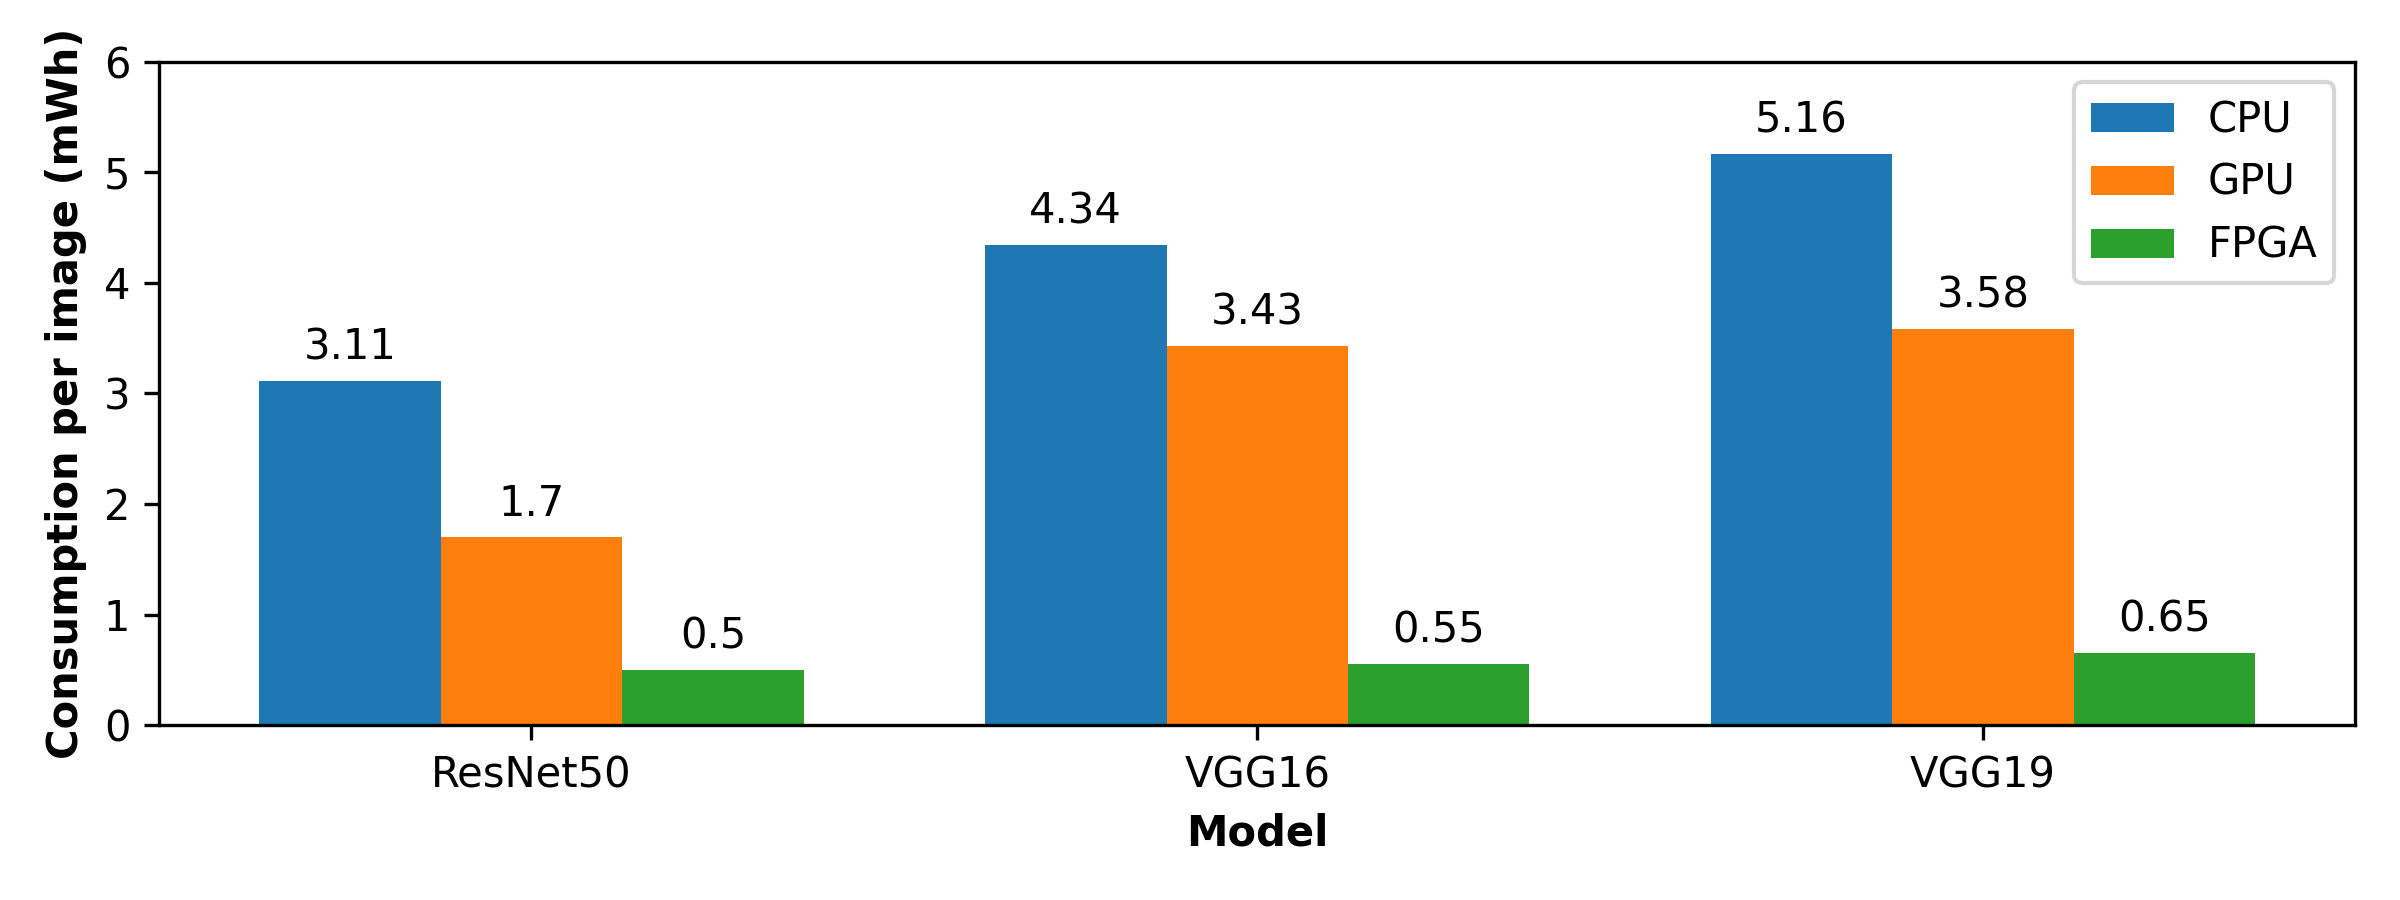
\includegraphics[width=\columnwidth]{5_Chapitre3/figures/characterization/consumption_per_image.png}
\caption{Energy consumption of inference per image (mWh).}
\label{figure:herofake-consumption-per-image}
\end{figure}

La consommation d'énergie instantanée mesurée pendant l'inférence est la consommation globale de la machine (y compris l'unité centrale, la mémoire, la carte mère et l'alimentation) pendant l'exécution de l'inférence. 
Les mesures ont été effectuées à l'aide d'une unité de distribution d'énergie (PDU) (Raritan PX3-5190R) capable de surveiller la puissance instantanée et la consommation d'énergie du serveur (Dell Precision T5810). Les résultats montrent que l'inférence sur le CPU produit la consommation d'énergie instantanée la plus faible. Ce résultat est assez attendu car l'inférence sur GPU ou FPGA inclut également la consommation d'énergie du CPU.


Cependant, la seule consommation d'énergie instantanée ne reflète pas correctement le coût total de chaque plateforme. Le temps d'exécution nécessaire pour traiter toutes les images doit être pris en compte. La mesure pertinente est le coût énergétique par image. La consommation d'énergie a été mesurée en kilowattheures (kWh) pour les 10 000 images, puis convertie en milliwattheures (mWh) par image. De ce point de vue, il est clair que le FPGA est le plus économe en énergie en ce qui concerne le temps d'exécution, consommant de 6,2 à 6,9 fois moins que le CPU et de 3,3 à 6,2 fois moins que le GPU (voir Figure~{figure:herofake-consumption-per-image}).

\subsection{Discussion}

\begin{figure}[t]
\centering
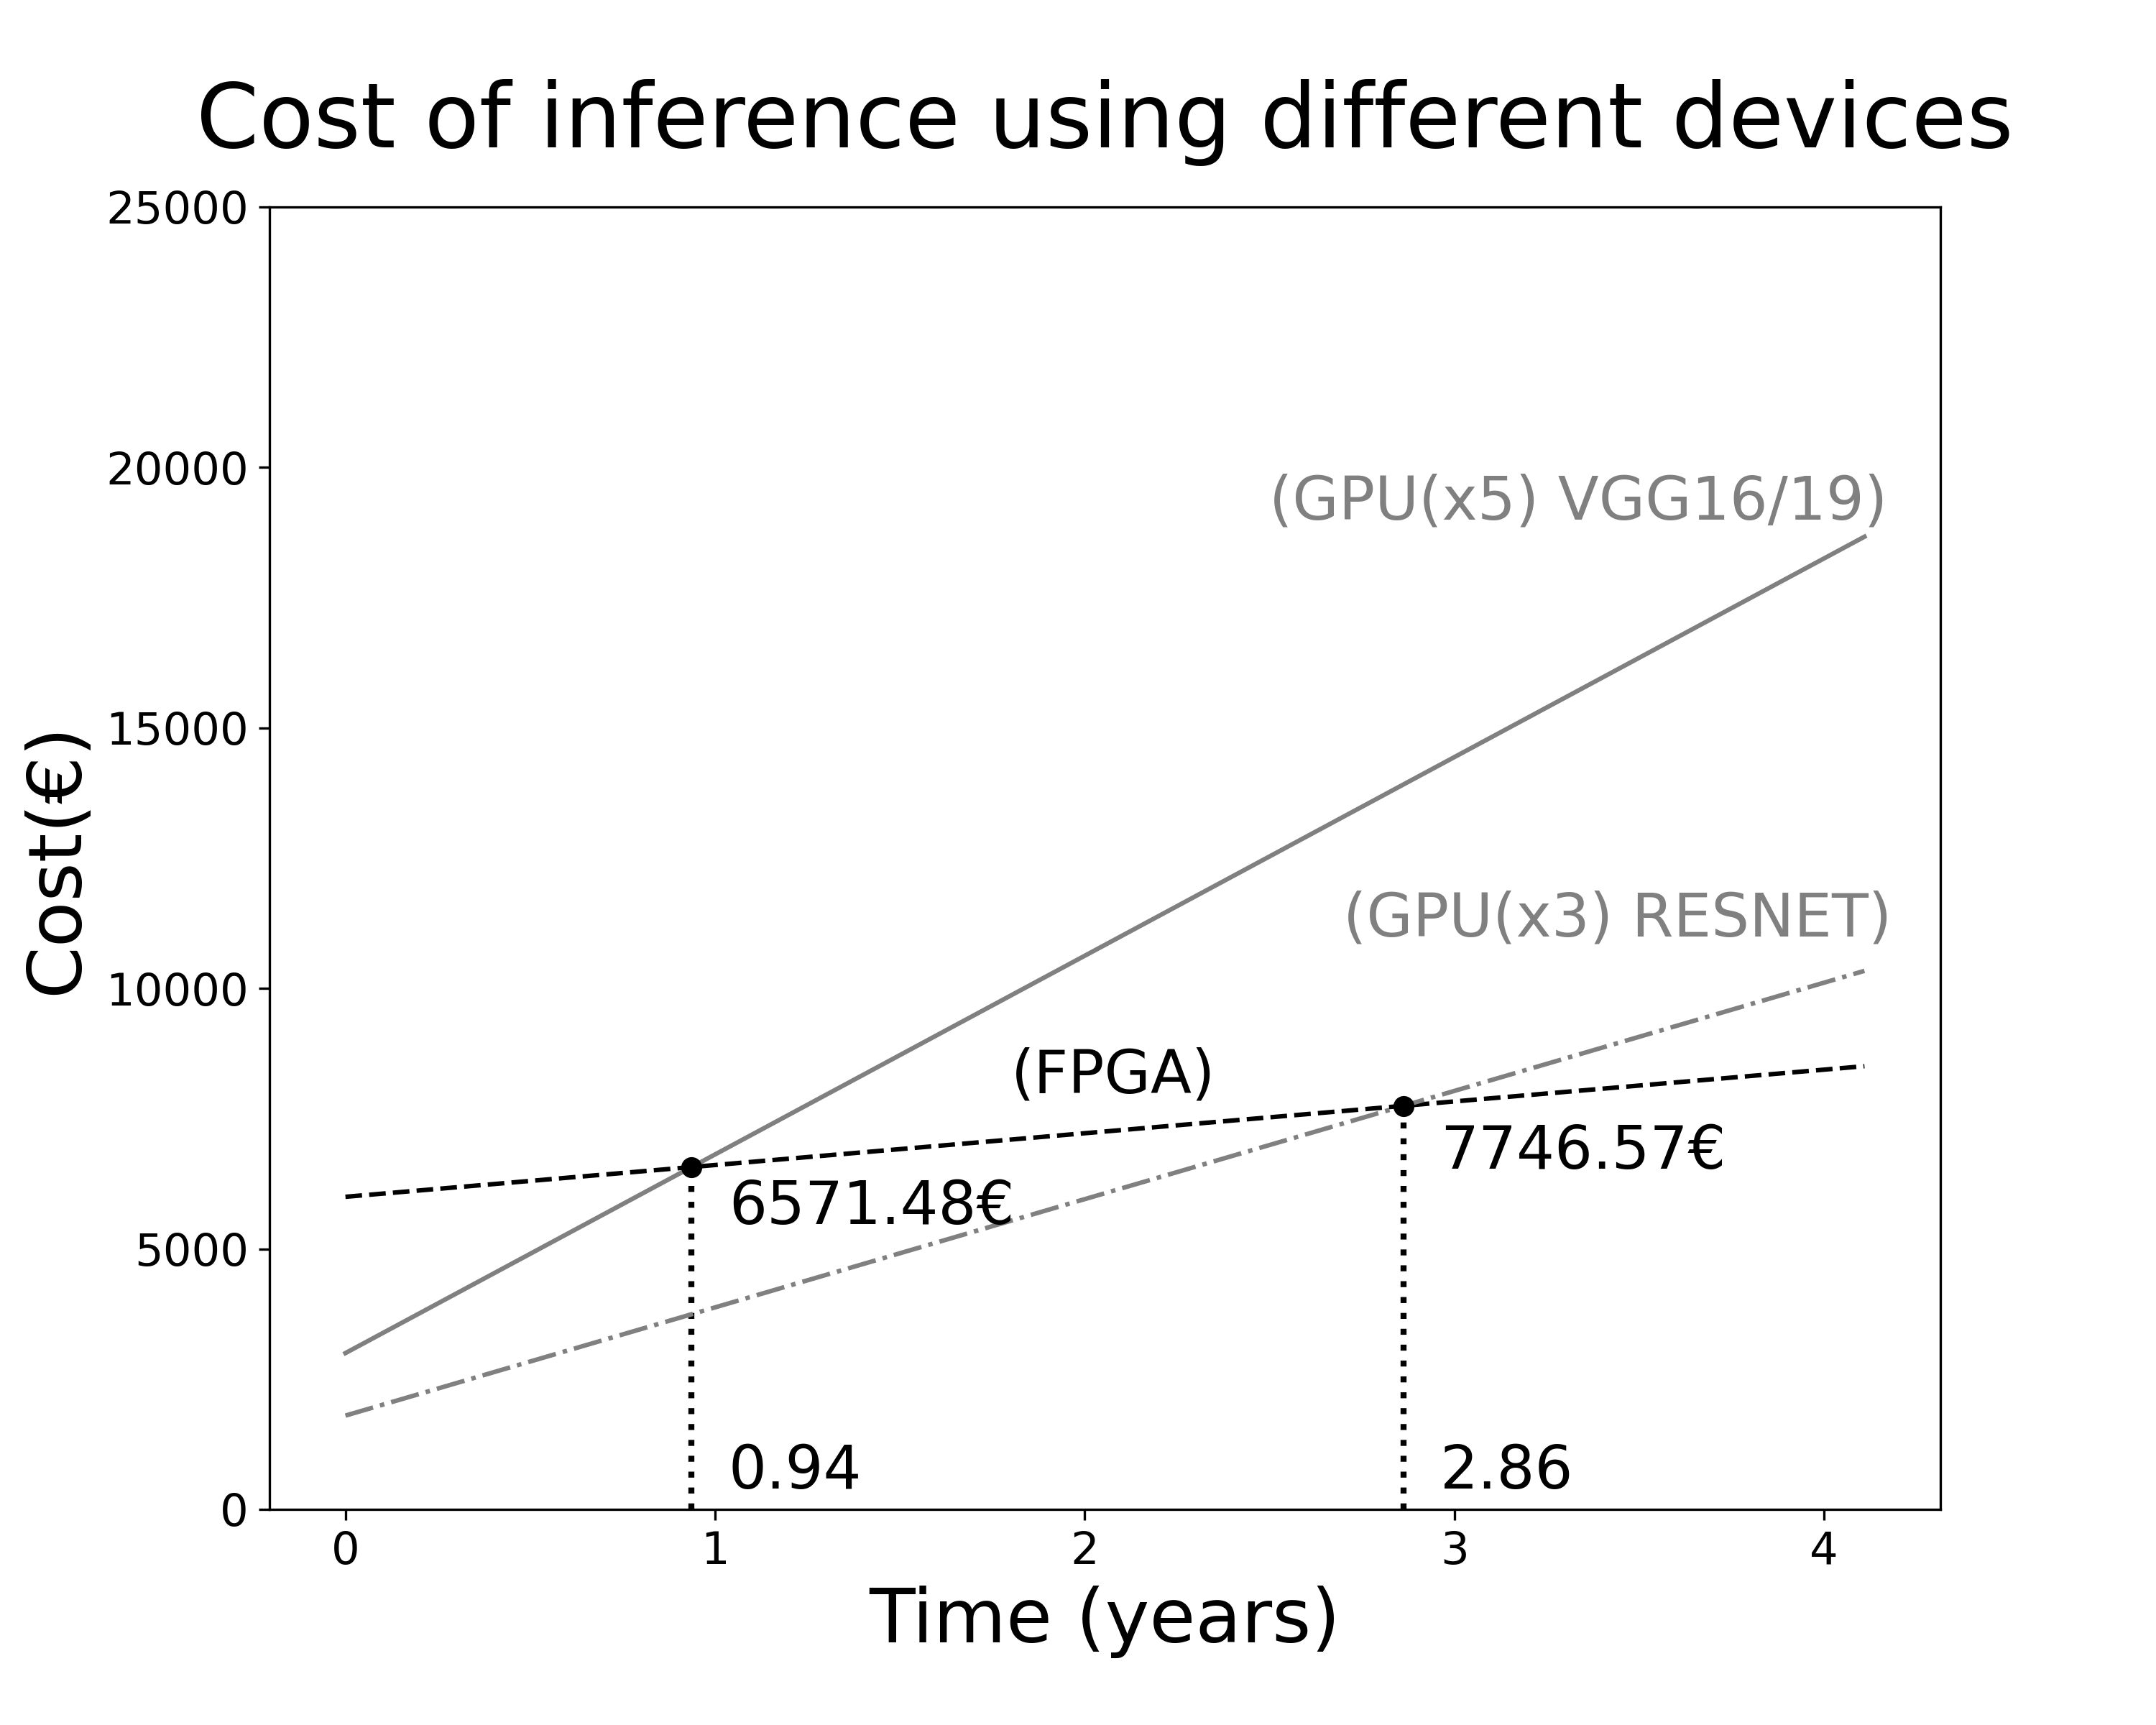
\includegraphics[scale=0.2]{5_Chapitre3/figures/characterization/cost_devices_time.png}
\caption{Total cost of inference on selected devices over time.}
\label{figure:herofake-cost-over-time}
\end{figure}

Les résultats de ce benchmark montrent un net avantage de l'inférence sur FPGA en termes de performance et d'efficacité énergétique. Les gains de performance sont significatifs, en particulier avec les réseaux d'apprentissage profond plus complexes~\cite{8782524}. Les ressources informatiques basées sur des serveurs équipés de cartes d'accélération FPGA, au lieu de cartes d'accélération GPU, bénéficieraient de ces avantages.

La consommation d'énergie brute du dispositif d'inférence ne reflète pas le coût total de la solution. En effet, il faut également inclure le coût de l'équipement lui-même. C'est un point important dans la comparaison entre GPU et FPGA, car il existe un écart de prix entre les deux technologies : le GPU (RTX 2070 Super) utilisé pour ce benchmark a été introduit aux alentours de 600€, alors que le FPGA (Alveo U250) est vendu aux alentours de 6000€. Le coût de l'énergie électrique pour effectuer l'inférence est très faible (nous avons utilisé la moyenne européenne de 0,1833 € par kWh proposée dans~\cite{energy-price}), comparé au coût initial du dispositif : la durée d'exécution nécessaire pour bénéficier de l'avantage de coût du FPGA est de l'ordre de plusieurs mois de fonctionnement continu. La figure~\ref{figure:herofake-cost-over-time} représente le coût cumulé (en euros) de l'utilisation d'un serveur avec accélération GPU ou FPGA en fonction du temps (en années). Notre estimation du coût comprend le nombre de GPU nécessaires et leur coût pour égaliser les performances des FPGA et utilise un facteur 2x~\cite{shehabiUnitedStatesData2016}, pour tenir compte de la consommation d'énergie totale de l'infrastructure (principalement le refroidissement et la mise en réseau). Le FPGA peut devenir une solution rentable après quelques mois pour les CNN complexes. Pour les réseaux moins complexes, l'avantage financier du FPGA est atteint après plus de deux ans.

\begin{figure}[t]
\centering
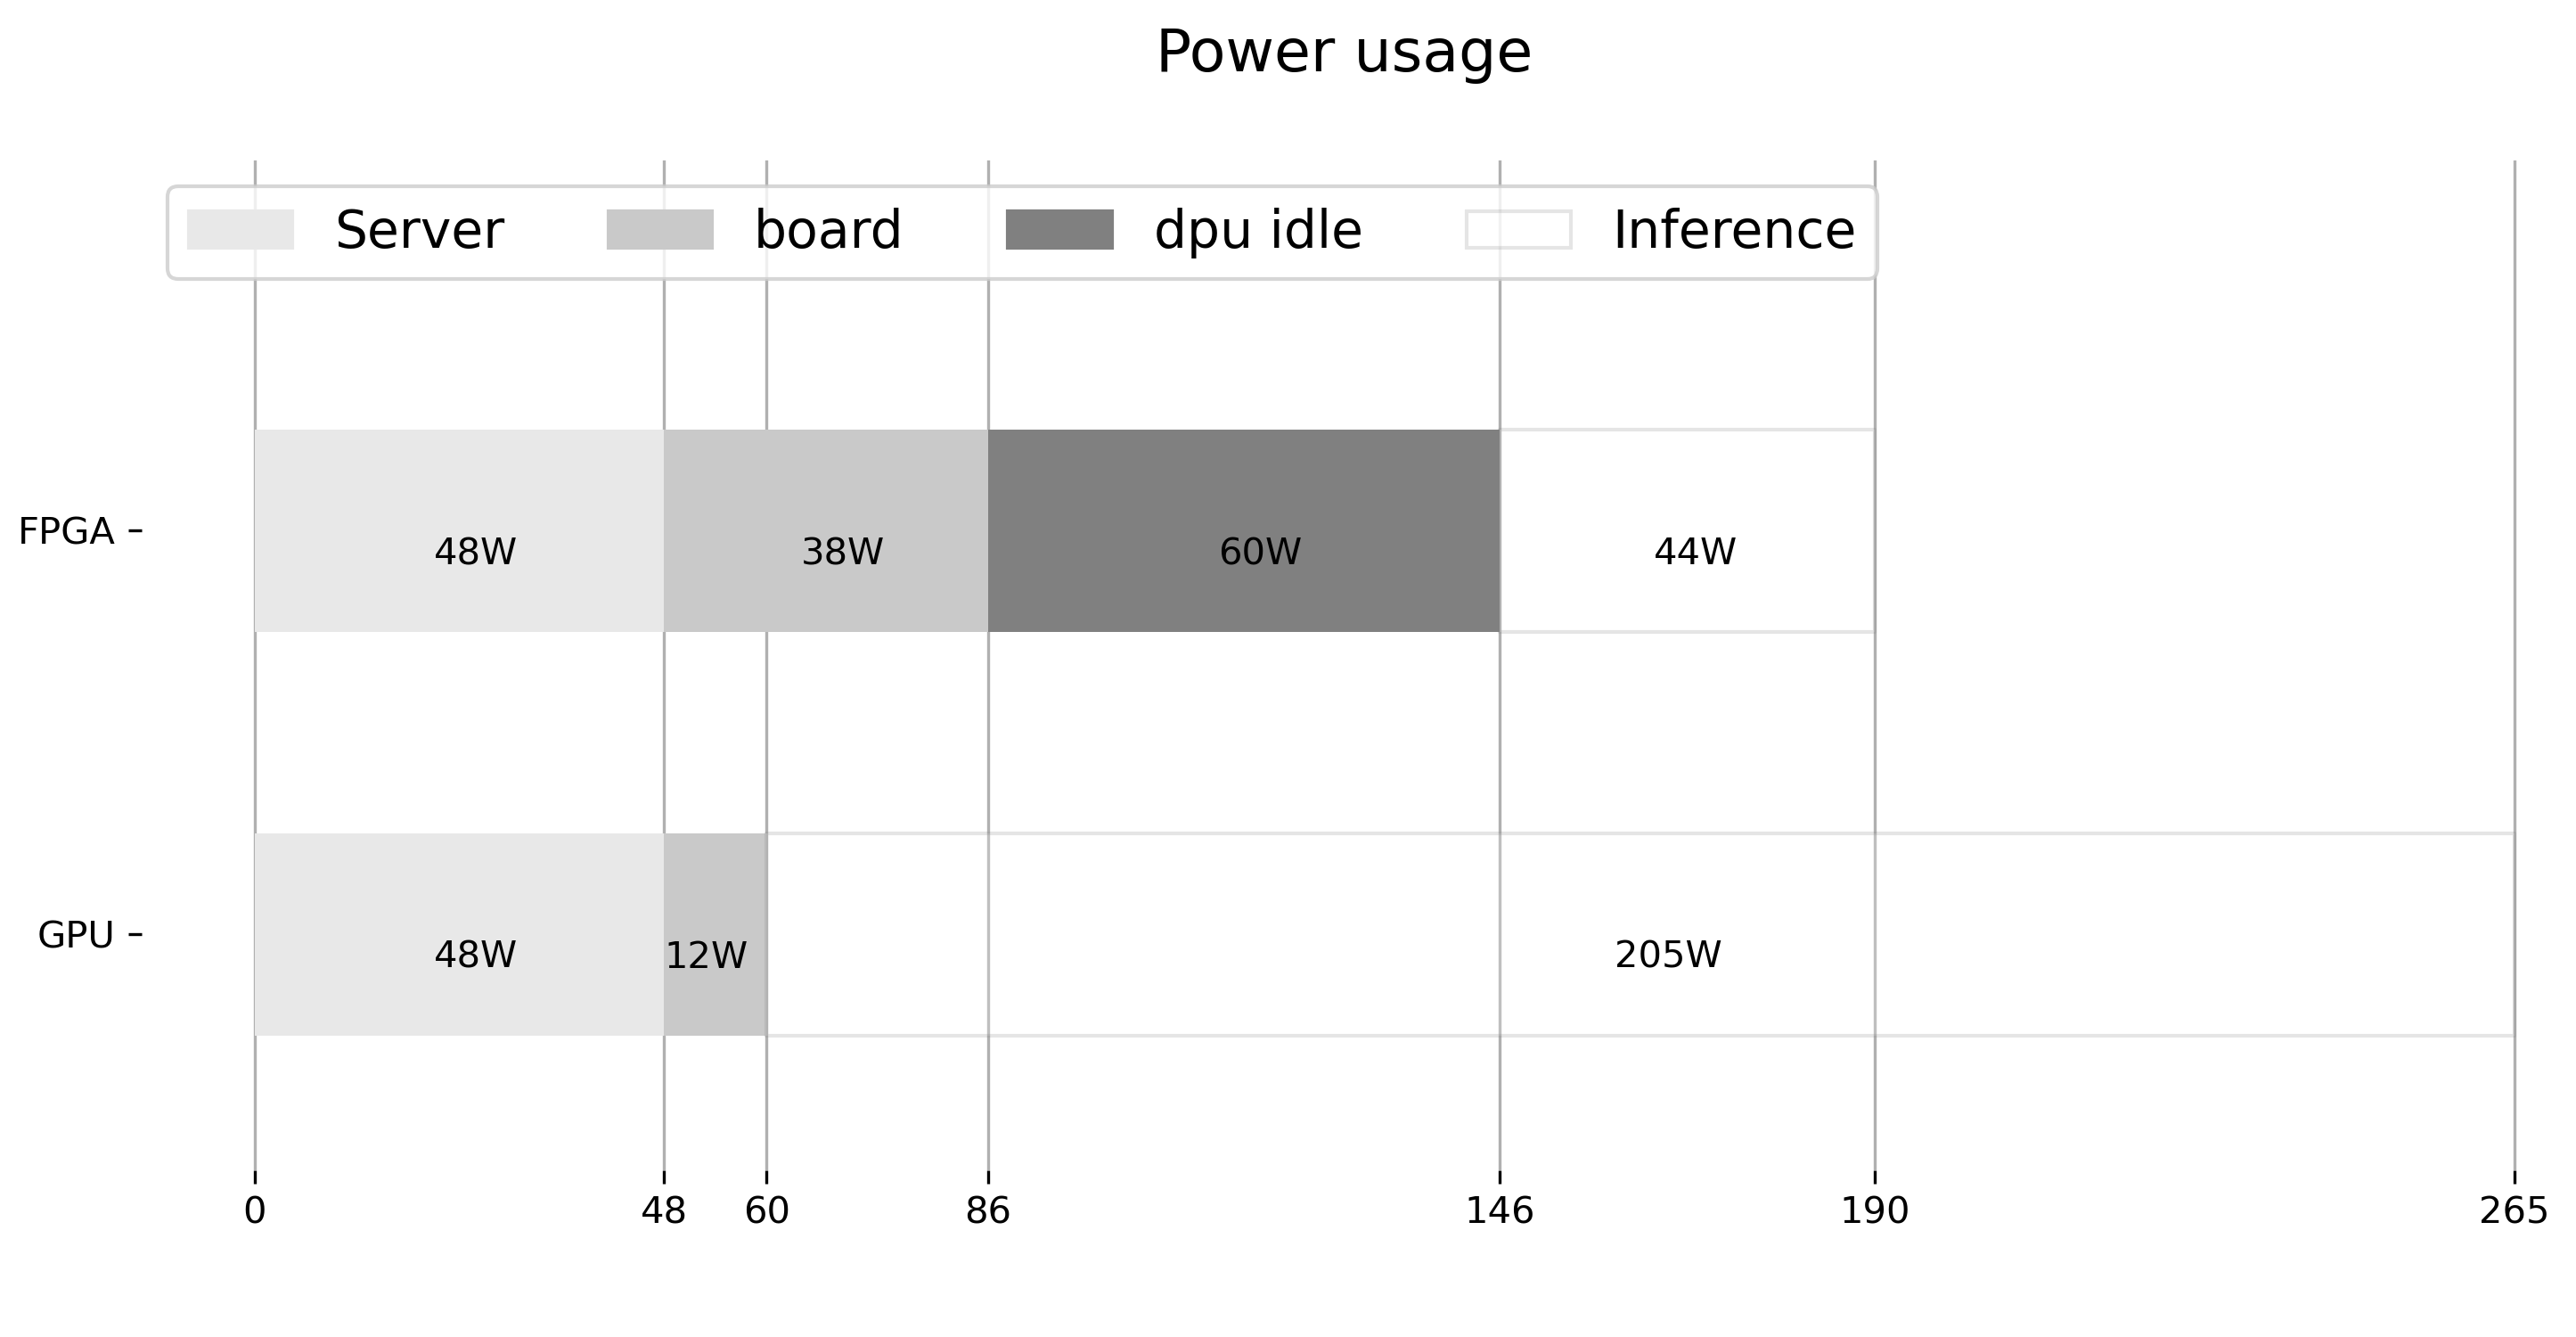
\includegraphics[width=\columnwidth]{5_Chapitre3/figures/characterization/power_usage.png}
\caption{Power usage breakdown for FPGA and GPU.}
\label{figure:herofake-power-usage}
\end{figure}

L'analyse précédente est valable dans le cas où l'inférence est toujours effectuée à pleine charge. En effet, lorsque l'on décompose la consommation d'énergie du GPU entre la consommation au repos et la consommation pour l'inférence, il est clair que le GPU est capable d'adapter dynamiquement sa consommation d'énergie à l'intensité du traitement. Le FPGA, quant à lui, semble avoir une gestion de l'énergie très limitée. Une fois que la conception du DPU est chargée dans le dispositif, sa consommation d'énergie au repos reste très élevée (voir la figure. \ref{figure:herofake-power-usage}). Si l'on ajoute les 38 W de la carte FPGA, il y a en effet une consommation résiduelle de 60 W lorsque le DPU est inactif. Même si l'évolution de l'implémentation du DPU sur le FPGA peut résoudre ce problème (par exemple en réduisant l'activité de l'arbre d'horloge lorsqu'il est inactif), cela a un impact sur le coût total et doit être pris en compte si le dispositif n'est pas toujours utilisé à pleine charge. Avec seulement 12 W d'énergie au repos, le GPU est un meilleur candidat lorsque l'utilisation à pleine charge du dispositif ne peut être garantie.

Comme la tendance vers des CNN plus complexes se poursuit~\cite{8807741}, l'utilisation des dispositifs les plus efficaces deviendra un défi majeur. La solution FPGA offre une nouvelle option pour effectuer l'inférence. Cependant, les FPGA ne remplacent pas encore les GPU : le flux de compilation reste complexe et prend du temps. Il faudra trouver un compromis entre la flexibilité des GPU et l'efficacité des FPGA. La section suivante traite d'un premier orchestrateur qui prend en compte la caractérisation mentionnée ci-dessus pour l'allocation et l'ordonnancement de ressources hétérogènes.

\section{Phase en ligne : allocation des ressources et placement des tâches}
\label{section:herofake-online}

Dans cette section, nous formulons le problème que notre contribution aborde, et nous donnons une description détaillée de notre modèle. Enfin, nous présentons une description formelle de notre stratégie pour la mise à l'échelle automatique des ressources et l'ordonnancement des tâches. 

\subsection{Défis pour l'orchestration dynamique}

L'ordonnancement des charges de travail dans le paradigme serverless est un problème à deux volets : les fournisseurs doivent gérer dynamiquement l'allocation des ressources (c'est-à-dire gérer les pools de ressources lors de la mise à l'échelle du nombre de répliques pour une application) et le placement des tâches (c'est-à-dire le mappage des tâches aux répliques existantes).

L'augmentation du nombre de répliques pose un problème de performance : lorsqu'une nouvelle réplique est créée, que ce soit sous la forme d'un conteneur ou d'une machine virtuelle, le bac à sable d'exécution doit passer par sa phase d'initialisation. C'est ce qu'on appelle un "démarrage à froid".

Les solutions commerciales telles que AWS Lambda évitent souvent le problème du démarrage à froid en maintenant des pools de bacs à sable préchauffés~\cite{vahidiniaColdStartServerless2020}. Ces machines virtuelles (VM) ou conteneurs sont démarrés par anticipation et mis en pause dans un état post-initialisation. Lorsque l'activité reprend, les demandes entrantes peuvent être servies sans souffrir d'un délai de démarrage à froid, au détriment du multiplexage des ressources du côté du fournisseur. Bien que cette solution permette de réduire, voire d'éliminer les délais de démarrage à froid, elle pèse sur la capacité de multiplexage des ressources du fournisseur et augmente le coût total de possession (TCO).

En outre, les applications de Machine Learning as a Service (MLaaS) présentent une charge très fluctuante~\cite{gujaratiSwayamDistributedAutoscaling2017}, ce qui renforce l'argument selon lequel une stratégie d'allocation des ressources réactive est nécessaire pour redimensionner l'infrastructure. Cependant, comme le temps d'exécution des tâches d'inférence est de l'ordre du centième ou du dixième de seconde, tandis que le temps d'initialisation des bacs à sable peut aller du centième de seconde à la seconde~\cite{mancoMyVMLighter2017}, nous avons besoin d'un mécanisme pour éviter d'encourir d'énormes coûts de latence pour l'exécution des fonctions.

Les tâches critiques nécessitent des garanties de niveau de service de la part du fournisseur. Les accords de niveau de service dans le cloud consistent généralement à convenir d'un taux de disponibilité des ressources dans le temps ; si le fournisseur ne respecte pas cet accord, une remise est proposée au client. Bien que cela puisse fonctionner pour des ressources réservées, nous pouvons voir que cela n'a pas de sens dans le paradigme serverless. La possibilité de garantir le temps de réponse des tâches permettrait à un fournisseur serverless d'atteindre des accords de niveau de service par invocation~\cite{zhangMArkExploitingCloud}.

L'utilisation d'accélérateurs matériels est une possibilité d'améliorer les rapports performance-coût. Bien qu'il s'agisse d'un investissement coûteux (voir Figure~\ref{figure:herofake-cost-over-time}), ces dispositifs permettent d'accélérer considérablement les tâches parallèles (voir Figure~\ref{figure:herofake-time-inference}), améliorant ainsi le temps de réponse des fonctions, avec un coût énergétique réduit (voir Figure~\ref{figure:herofake-consumption-per-image}).

\subsection{Modèle de tâche} \label{model:tasks}

\begin{table}[t]
    \caption{Notation dictionary}
    \begin{center}
    \begin{tabular}{|c|L|}
    \hline
    \textbf{Notation} & \textbf{Description} \\ \hline
    $f_{N, P}$ & A function $f$ scheduled to run on a platform $P$ available on node $N$ \\ \hline
    $QP$ & QoS penalty \\ \hline
    $QD$ & QoS deviation \\ \hline
    $WET$ & Worst execution time \\ \hline
    $TT$ & Task total time \\ \hline
    $WT$ & Wait time \\ \hline
    $CST$ & Cold start time \\ \hline
    $ET$ & Execution time \\ \hline
    $EC$ & Energy consumption \\ \hline
    $HP$ & Hardware price \\ \hline
    $TC$ & Task consolidation \\ \hline
    $Q$ & Task queue on a replica \\ \hline
    $replicaCount_{f}$ & Size of the replica pool in the system for a function $f$ \\ \hline
    $concurrency_{f}$ & Average number of in-flight requests for a function $f$ \\ \hline
    $threshold$ & Concurrency threshold for function replicas in vanilla Knative \\ \hline
    $replicaCount_{f, h}$ & Size of the replica pool for a function $f$ on hardware type $h$ \\ \hline
    $concurrency_{f, h}$ & Average number of in-flight requests for a function $f$ on replicas of hardware type $h$ \\ \hline
    $x_{f, h}$ & Concurrency threshold for a function $f$ on a replica of hardware type $h$ \\ \hline
    $scaleCost_{{f}_{N, P}}$ & Cost of creating a new replica for function $f$ on a platform $P$ available on node $N$ \\ \hline
    $schedCost_{{f}_{N, P}}$ & Cost of scheduling an execution of function $f$ on a platform $P$ available on node $N$ \\ \hline
    \end{tabular}
    \label{table:herofake-notation}
    \end{center}
\end{table}

Les applications sont composées de fonctions. L'exécution d'une fonction est appelée \textit{tâche}. Dans ce travail, il n'y a pas de dépendances entre ces tâches : l'application est composée de fonctions pures et sans état. Les événements qui déclenchent l'exécution d'une tâche arrivent dans le système à un intervalle aléatoire et borné. Nous formulons l'hypothèse qu'une requête aboutit toujours et conduit à l'exécution d'une \textit{task} (une instance de \textit{fonction}). Lorsqu'une tâche a commencé son exécution sur la plateforme qui lui a été attribuée, elle s'exécute pendant la totalité de son temps d'exécution. Nous ne prenons pas en compte la préemption ou les défaillances dans cette contribution : une tâche termine toujours son exécution avec succès, même si son temps de réponse peut dépasser ses exigences en matière de qualité de service. Nous ne tenons pas compte des interférences possibles entre les charges de travail sur le même nœud~\cite{dartoisInvestigatingMachineLearning2021}. 

Nous considérons les tâches qui peuvent être exécutées sans distinction sur des plateformes d'exécution hétérogènes. Dans le contexte de notre étude de cas spécifique, la mise en œuvre des différentes fonctions a été effectuée à la main pour chaque plateforme ; cependant, des travaux existent pour permettre une compilation croisée automatique pour les architectures hétérogènes~\cite{hortaXartrekRuntimeExecution2021, 10.1145/3445814.3446699}. Les métadonnées suivantes ont été mesurées pour chaque fonction, sur chaque plateforme d'exécution : 

\begin{itemize}
    \item \textit{Besoins mémoire en pic} -- la quantité de mémoire (en GB) allouée à la tâche ;
    \item \textit{Durée de démarrage à froid} -- la durée de l'initialisation du bac à sable lors de l'exécution de la tâche sur une plateforme qui n'a pas la fonction en cache ;
    \item \textit{Temps d'exécution} -- la durée prévue de l'exécution effective de la tâche, à l'exclusion de sa phase d'initialisation ;
    \item \textit{Consommation d'énergie} -- la différence entre l'énergie inactive et l'énergie active encourue par la plateforme d'exécution lorsqu'elle exécute la tâche.
\end{itemize}

L'équation~\ref{eq:herofake-HRO-total-time} décompose le temps de réponse attendu pour l'exécution d'une fonction $f$ sur une plateforme $P$ sur un nœud $N$.

\begin{equation}
    {TT}_{{f}_{N, P}} = {WT}_{{f}_{N, P}} + {CST}_{{f}_{N, P}} + {ET}_{{f}_{N, P}}
\label{eq:herofake-HRO-total-time}
\end{equation}

Où :

\begin{itemize}
    \item ${WT}_{{f}_{N, P}}$ correspond à la durée de la décision d'ordonnancement, y compris le temps passé par la requête en file d'attente ;
    \item ${CST}_{{f}_{N, P}}$ est la durée de l'initialisation de l'invocation de la fonction, y compris son temps potentiel de démarrage à froid ;
    \item ${ET}_{{f}_{N, P}}$ est le temps d'exécution de la fonction sur la plateforme.
\end{itemize}

Nous proposons différents niveaux de qualité de service en fonction des besoins des utilisateurs en termes de garanties sur le temps d'exécution. Chaque niveau de qualité de service présente un \textit{écart de durée} différent (noté $QD$ dans l'équation~\ref{eq:herofake-task-penalty}) -- un facteur par lequel le pire temps d'exécution d'une fonction est multiplié pour donner une limite supérieure au temps d'exécution de cette fonction pour ce niveau de qualité de service.

Le temps d'exécution prédit d'une fonction est toujours basé sur le pire temps d'exécution (noté $WET_{f}$), c'est-à-dire le temps d'exécution d'une tâche lorsqu'elle est programmée sur la plateforme d'exécution présentant le niveau de performance le plus faible pour cette fonction :


\begin{equation}
    \forall \, (N, P), \, WET_{f} = \max ET_{N, P}
\label{eq:herofake-task-wet}
\end{equation}

Une fois qu'une tâche est programmée sur une plateforme d'exécution, elle passe par sa durée totale d'exécution décrite dans l'équation \ref{eq:herofake-HRO-total-time}. L'échéance de la tâche est calculée en multipliant le pire temps de réponse de la fonction (tel qu'exprimé dans l'équation~\ref{eq:herofake-task-wet}) par l'écart de durée de la qualité de service associé au niveau de qualité de service de la demande de l'utilisateur. L'équation~\ref{eq:herofake-task-penalty} montre que nous fixons une valeur booléenne $QP_{f_{N, P}}$ pour chaque invocation de fonction si la tâche ne respecte pas son délai. 


\begin{equation}
    QP_{f_{N, P}} = TT_{f_{N, P}} \cdot QD_{f_{N, P}} > WET_{f}
\label{eq:herofake-task-penalty}
\end{equation}

\subsection{Stratégie d'allocation de ressources} \label{section:herofake-autoscaling-strategy}

Dans une plateforme serverless, l'autoscaler a la responsabilité d'allouer des ressources matérielles pour les exécutions de fonctions. Pour toute fonction, un autoscaler peut allouer $n$ \textit{répliques}. Le nombre de répliques pour une fonction donnée à un moment donné détermine le niveau de concurrence.

Dans Knative, le nombre de répliques pour une fonction donnée (équation~\ref{eq:herofake-kn-replica-count}) dépend de la charge moyenne mobile pour une fonction, c'est-à-dire le nombre moyen de requêtes en vol pour la fonction sur une fenêtre de 60 secondes (concurrence dans le système par fonction). Il est limité par un seuil de concurrence par réplique, c'est-à-dire le nombre maximum de demandes en file d'attente dans la réplique d'une fonction à tout moment. La valeur par défaut dans Knative est de 100 requêtes en vol dans chaque réplique~\cite{knative-autoscaling}.

\begin{equation}
    replicaCount_{f} = \frac{concurrency_{f}}{threshold}
\label{eq:herofake-kn-replica-count}
\end{equation}

Ce mécanisme de dimensionnement permet d'allouer des CPU sous Knative, en réaction aux changements de l'état actuel de la concurrence dans le système. La principale contribution de l'autoscaler que nous proposons est d'améliorer Knative afin de prendre en compte l'hétérogénéité des plateformes d'exécution.

Le mécanisme Knative simple ne fonctionne pas lorsque l'infrastructure est constituée d'une variété de plateformes d'exécution. En effet, ces plateformes présentent différents niveaux de performance, de consommation d'énergie et de coût. Cela a une conséquence sur le nombre de répliques que le fournisseur doit déployer sur ces plateformes : pour un niveau donné de charge d'application, les répliques hétérogènes seront capables de traiter différents nombres de tâches dans le même délai. Pour que notre plateforme puisse gérer l'hétérogénéité de l'infrastructure sous-jacente, nous proposons un nombre de répliques par fonction et \textbf{par type de matériel} comme dans l'équation~\ref{eq:herofake-HRO-replica-count}.

\begin{equation}
    replicaCount_{f, h} = \frac{concurrency_{f, h}}{x_{f, h}}
\label{eq:herofake-HRO-replica-count}
\end{equation}

Une décision d'autoscaling peut introduire des coûts d'opportunité dans le système : les accélérateurs matériels sont peu disponibles par rapport aux CPU, et le fait de les allouer à une fonction donnée à un moment donné les rendra indisponibles pour d'autres calculs. Pour que l'autoscaler puisse décider quand il est pertinent d'allouer de tels accélérateurs, il doit être conscient des coûts. 

Afin de déterminer le seuil de concurrence par réplique $x_{f, h}$ pour une fonction $f$ sur un type de matériel $h$ (par exemple, GPU et FPGA), nous avons fixé le seuil de concurrence par réplique sur les CPU à $x_{f, c} = 100$, comme c'est la valeur par défaut dans Knative~\cite{knative-concurrency}. Ensuite, nous avons utilisé les mesures de la phase hors-ligne (Table~\ref{table:herofake-tasks}) pour établir un ratio composite (incluant la performance, l'énergie, le prix de la plateforme) comme décrit dans l'équation~\ref{eq:herofake-HRO-concurrency-target}. Dans notre politique, nous avons choisi de favoriser le temps de réponse en fixant $k_{ET} = \frac{2}{3}$, $k_{EC} = \frac{1,5}{6}$ et $k_{HP} = \frac{0,5}{6}$. Par exemple, pour la fonction ResNet50 (décrite dans Table~\ref{model:tasks}), les files d'attente de tâches dans les réplicas sont dimensionnées à 100 pour les CPU, 489 pour les GPU et 1292 pour les FPGA.

\begin{equation}
    x_{f, h} = x_{f, c} \cdot (k_{ET} \cdot \frac{ET_{{f}_{c}}}{ET_{{f}_{h}}} + k_{EC} \cdot \frac{EC_{{f}_{c}}}{EC_{{f}_{h}}} + k_{HP} \cdot \frac{HP_{{f}_{c}}}{HP_{{f}_{h}}})
\label{eq:herofake-HRO-concurrency-target}
\end{equation}

Lorsque le seuil de simultanéité d'une fonction est dépassé dans les files d'attente des répliques sur un type de matériel donné, l'autoscaler procède à la \textit{scale out} de la fonction : une nouvelle réplique est mise en route pour traiter les demandes ultérieures des utilisateurs.

L'allocation commence par la liste complète des nœuds disponibles dans l'infrastructure. Nous commençons par constituer un sous-ensemble de nœuds disponibles, appelé \textit{nœuds appropriés}. Compte tenu des besoins en mémoire que nous avons mesurés pour chaque fonction, nous éliminons les nœuds qui ne disposent pas actuellement de suffisamment de mémoire pour exécuter une réplique de la fonction. Chaque réplique déployée sur la plateforme d'exécution d'un nœud consomme la quantité totale de mémoire requise par le type de fonction. Si le nœud n'a plus de mémoire, ses plateformes d'exécution ne peuvent plus être utilisées pour déployer d'autres répliques.

Afin de sélectionner le type de ressource à allouer à cette réplique, l'autoscaler minimise la fonction de coût donnée dans l'équation~\ref{eq:herofake-HRO-allocation-cost-function}. 
Dans notre politique, comme pour l'autoscaling, nous avons choisi de favoriser le temps total d'exécution des tâches en fixant $k_{TT} = \frac{2}{3}$, $k_{EC} = \frac{1.5}{6}$ et $k_{HP} = \frac{0.5}{6}$. 
En fonction du matériel disponible dans le pool au moment de la mise à l'échelle, l'autoscaler favorisera la création d'une nouvelle réplique de fonction sur la plateforme qui exécutera la tâche dans le temps total le plus court, y compris le démarrage à froid, avec la consommation d'énergie la plus faible et le prix le plus bas.

\begin{equation}
\begin{split}
    scaleCost_{{f}_{N, P}} = \, &k_{TT} \cdot {TT}_{{f}_{N, P}} \\
    + &k_{EC} \cdot {EC}_{{f}_{N, P}} \\
    + &k_{HP} \cdot {HP}_{{f}_{N, P}}
\end{split}
\label{eq:herofake-HRO-allocation-cost-function}
\end{equation}

Au contraire, lorsque la concurrence pour une fonction tombe en dessous du seuil sur un type de matériel donné, l'autoscaler emploiera une politique de meilleur effort et essaiera de désallouer tout réplica avec une file d'attente de tâches vide sur ce type de matériel. Si une réplique a une file d'attente de tâches vide, elle sera libérée dans le pool de plates-formes disponibles et la mémoire qui lui avait été allouée sur le nœud sera libérée.

Les différents poids ($k$) utilisés dans les équations~\ref{eq:herofake-HRO-concurrency-target} et~\ref{eq:herofake-HRO-allocation-cost-function} peuvent être modifiés par le fournisseur afin de personnaliser la politique d'allocation en fonction de différentes priorités.

\subsection{Stratégie d'ordonnancement} \label{section:herofake-scheduling-strategy}

La caractérisation de la charge de travail est essentielle à la prédiction des performances, car elle peut guider les décisions d'ordonnancement qui conduisent à la satisfaction des exigences de qualité de service~\cite{mampageHolisticViewResource2022}. Notre stratégie d'ordonnancement s'appuie sur les métadonnées des tâches décrites dans la section~\ref{model:tasks}. La construction de connaissances sur les tâches serverless est réalisée au cours d'une phase hors-ligne sur notre plateforme, car le code est poussé vers les registres du fournisseur avant l'exécution réelle~\cite{shahradServerlessWildCharacterizing}.

Dans Knative, le planificateur gère les tâches entrantes de manière FIFO. Pour gérer les différents niveaux d'exigences en matière de qualité de service, nous proposons que notre ordonnanceur retire les tâches de la file d'attente de l'orchestrateur par \textbf{échéance la plus proche}. Nous calculons l'échéance de la tâche en utilisant sa pire durée d'exécution sur la plateforme à l'aide de l'équation~\ref{eq:herofake-task-wet}, et en la multipliant par l'écart de durée autorisé fixé par le niveau de qualité de service. Après l'exécution de la tâche, nous vérifierons si nous avons dépassé son échéance et fixerons la pénalité associée en conséquence, comme décrit dans l'équation~\ref{eq:herofake-task-penalty}. 

Nous itérons sur les répliques de la fonction pour récupérer et prédire les métriques suivantes basées sur les métadonnées de la tâche :

\begin{itemize}
    \item \textbf{pénalité potentielle} : nous calculons la longueur de la file d'attente de la plateforme et vérifions si l'échéance de la tâche sera dépassée, comme décrit dans l'équation~\ref{eq:herofake-task-penalty} ;
    \item \textbf{consommation d'énergie} : nous récupérons les mesures hors-ligne pour établir la consommation d'énergie dynamique de cette tâche sur la plateforme ;
    \item \textbf{fusion des tâches} : nous calculons la longueur de la file d'attente des tâches de la plateforme $Q$ en additionnant les durées totales de toutes les tâches en file d'attente, comme décrit dans les équations~\ref{eq:herofake-HRO-scheduling-platform-queue} (longueur de la file d'attente) et~\ref{eq:herofake-HRO-total-time} (durée totale de la tâche). 
\end{itemize}

\begin{equation}
    len \, Q_{N, P} = \sum TT_{f_{N, P}}
\label{eq:herofake-HRO-scheduling-platform-queue}
\end{equation}

Ces valeurs sont normalisées pour s'adapter à une fonction de coût pondérée décrite dans l'équation~\ref{eq:herofake-HRO-scheduling-cost-function}. Nous avons utilisé $k_{QP} = \frac{2}{3}$, $k_{EC} = \frac{0.5}{6}$ et $k_{TC} = \frac{1.5}{6}$ (comme pour l'autoscaler). L'ordonnanceur minimise ensuite cette fonction de coût pour toutes les répliques $(N, P)$ (c'est-à-dire le nœud et la plateforme d'exécution).

\begin{equation}
\begin{split}
    schedCost_{{f}_{N, P}} = \, &k_{QP} \cdot QP_{{f}_{N, P}} \\
    + &k_{EC} \cdot {EC}_{{f}_{N, P}} \\
    + &k_{TC} \cdot TC_{{f}_{N, P}}
\end{split}
\label{eq:herofake-HRO-scheduling-cost-function}
\end{equation}

Si l'ordonnanceur ne trouve pas de réplique disponible pour exécuter la tâche, celle-ci sera repoussée dans la file d'attente de l'orchestrateur. Cela augmentera la concurrence dans le système pour la fonction, poussant l'autoscaler à allouer une autre réplique sur le matériel approprié.

\section{Évaluation}
\label{section:herofake-evaluation}

\begin{figure*}[t]
    \centering
    \subfloat[Task consolidation (based on the unused node count)\label{figure:herofake-evaluation-full-nodes}]{
        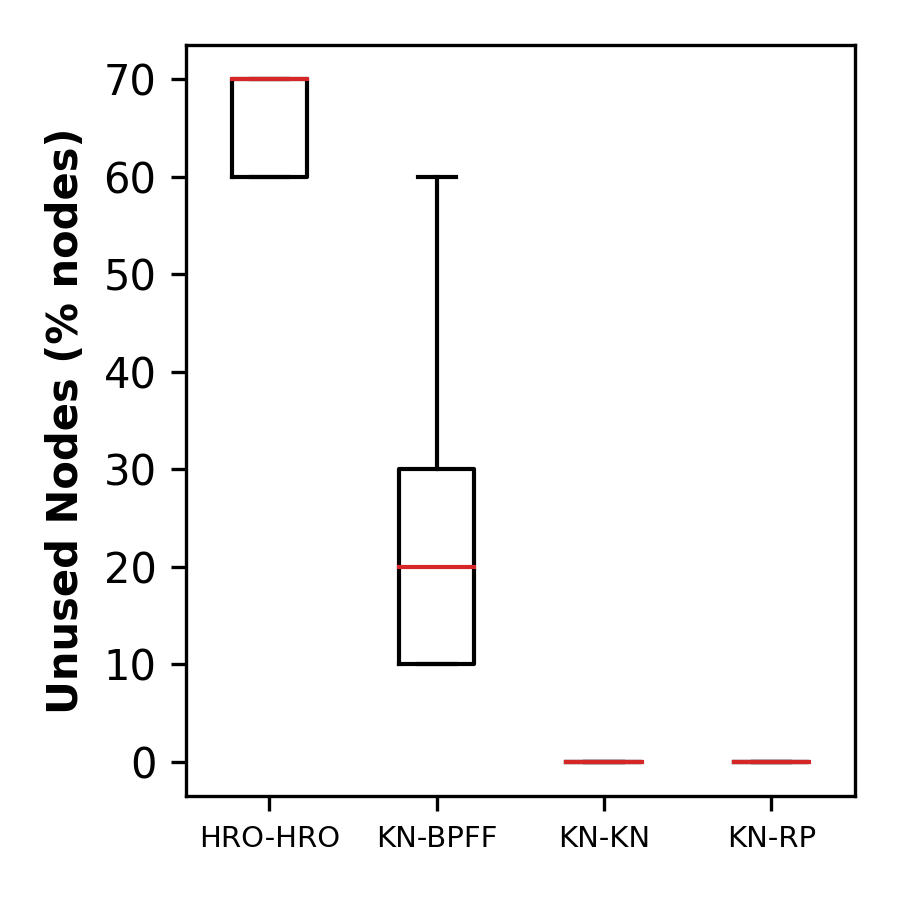
\includegraphics[width=0.28\linewidth]{5_Chapitre3/figures/evaluation/z-nodes-20221212-232143-169224.png}
    }\qquad
    \subfloat[QoS violations (based on tasks with missed deadline)\label{figure:herofake-evaluation-full-penalty}]{
        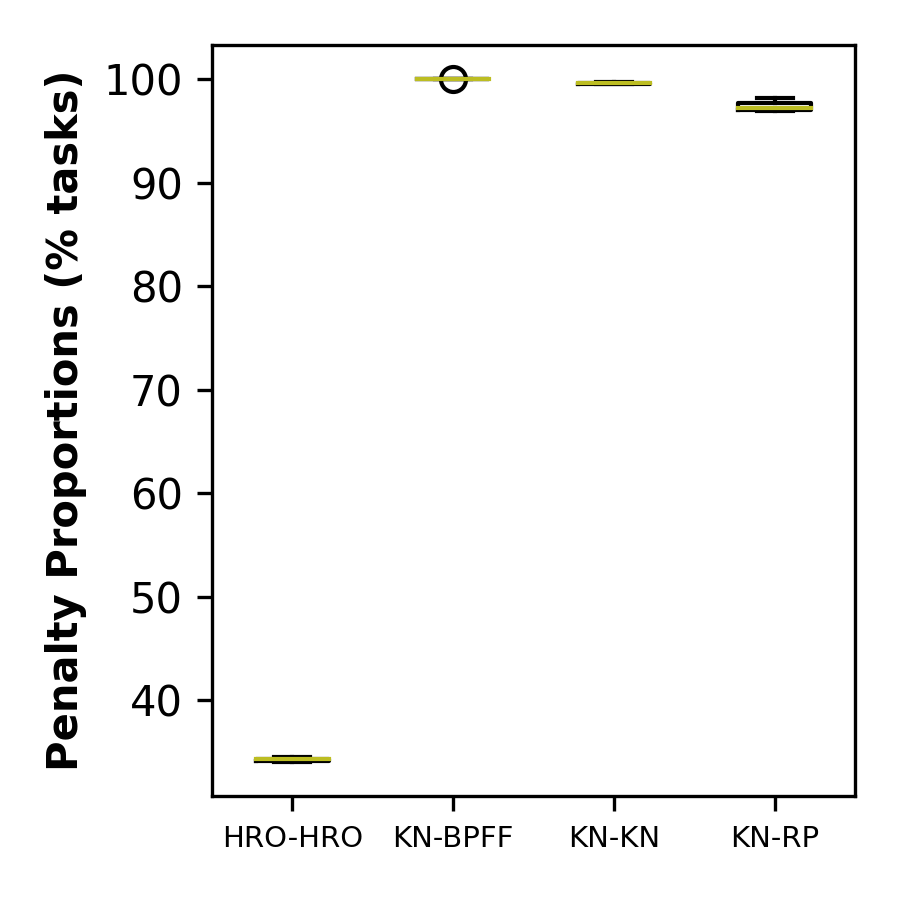
\includegraphics[width=0.28\linewidth]{5_Chapitre3/figures/evaluation/z-penalty-20221212-232143-169224.png}
    }\qquad
    \subfloat[Dynamic energy consumption (in kWh)\label{figure:herofake-evaluation-full-energy}]{
        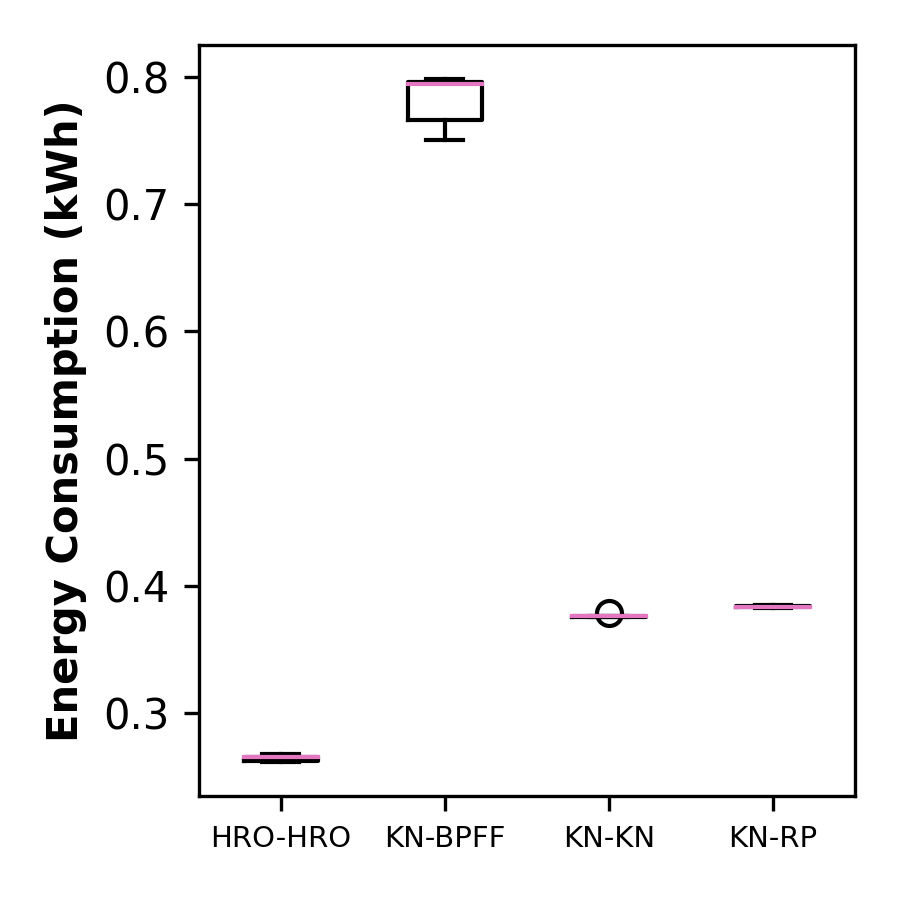
\includegraphics[width=0.28\linewidth]{5_Chapitre3/figures/evaluation/z-energy-20221212-232143-169224.png}
    }
    \caption{Evaluation 1 -- Comparison against baselines}
    \label{figure:herofake-evaluation-hro-full}
\end{figure*}

\begin{figure*}[t]
    \centering
    \subfloat[Task consolidation (based on the unused node count)\label{figure:herofake-evaluation-mixed-nodes}]{
        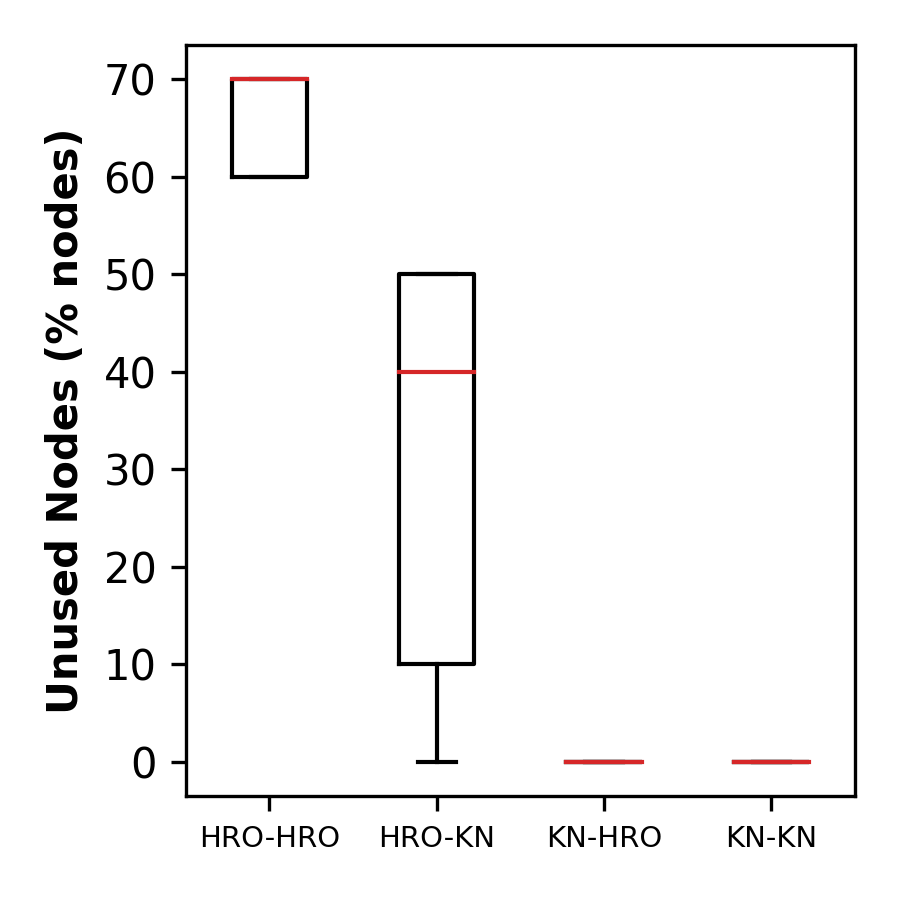
\includegraphics[width=0.28\linewidth]{5_Chapitre3/figures/evaluation/x-nodes-20221212-185844-053283.png}
    }\qquad
    \subfloat[QoS violations (based on tasks with missed deadline)\label{figure:herofake-evaluation-mixed-penalty}]{
        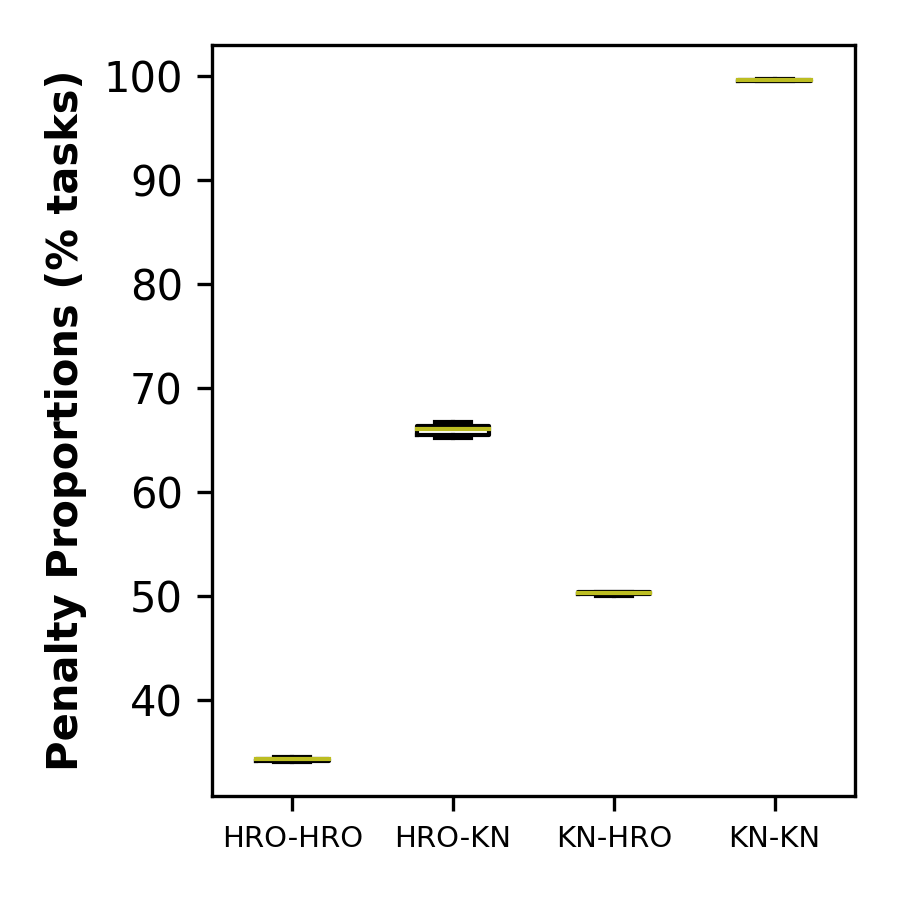
\includegraphics[width=0.28\linewidth]{5_Chapitre3/figures/evaluation/x-penalty-20221212-185844-053283.png}
    }\qquad
    \subfloat[Dynamic energy consumption (in kWh)\label{figure:herofake-evaluation-mixed-energy}]{
        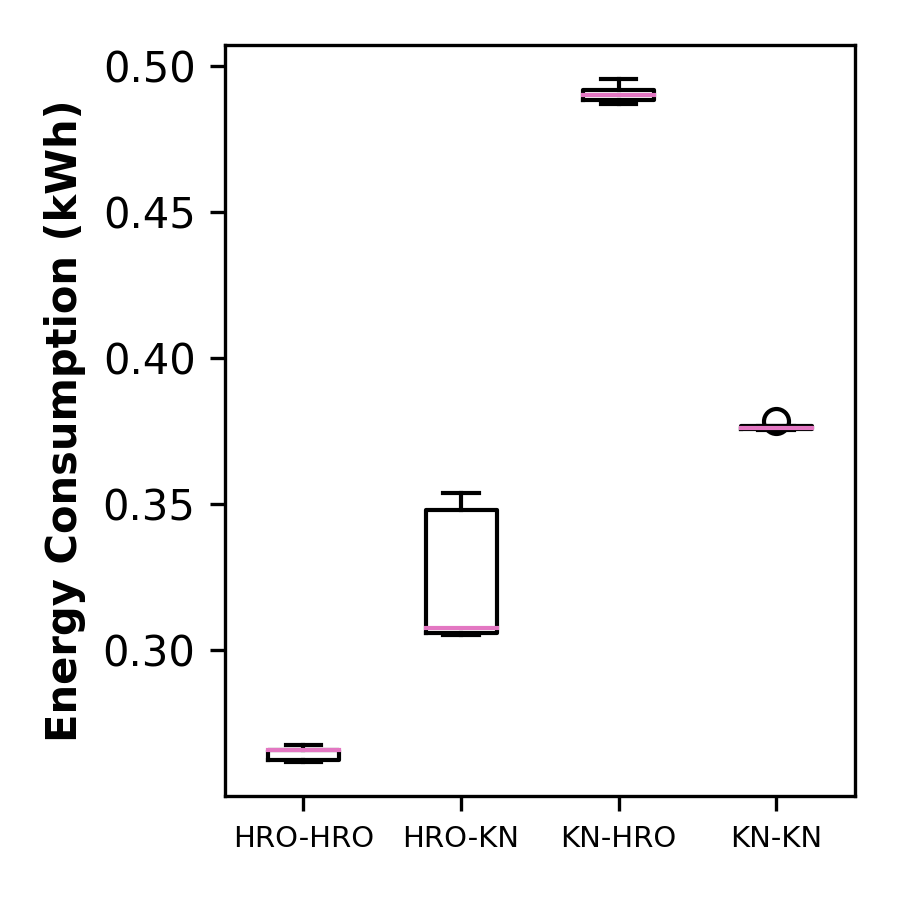
\includegraphics[width=0.28\linewidth]{5_Chapitre3/figures/evaluation/x-energy-20221212-185844-053283.png}
    }
    \caption{Evaluation 2 -- Impact of HeROfake components on the overall performance}
    \label{figure:herofake-evaluation-hro-mixed}
\end{figure*}

\subsection{Protocole expérimental}

Nous avons utilisé des mesures provenant de l'évaluation de trois modèles d'apprentissage automatique différents (voir Tableau~\ref{table:herofake-tasks}). Ces modèles ont été mis en œuvre sur trois plateformes d'exécution différentes (voir Tableau~\ref{table:herofake-platforms}) comme expliqué dans la Section~\ref{section:herofake-offline}.

Ces données ont servi d'entrée à un simulateur que nous avons construit en utilisant SimPy~\cite{simpy}. Le simulateur suit le modèle de système décrit dans les sections~\ref{model:nodes}, \ref{model:platforms}, \ref{model:tasks}.

Nous avons mesuré les délais de démarrage à froid pour les applications de notre étude de cas, voir le tableau~\ref{table:herofake-tasks}. Il apparaît que les délais d'exécution sont dominés par les délais de démarrage à froid, ce qui fait de l'allocation adéquate des ressources une exigence stricte pour respecter les accords de niveau de service.

Dans la partie consacrée à l'évaluation des performances, nous comparons deux autoscalers :

\begin{itemize}
    \item HeROfake (HRO) -- Notre allocateur de ressources basé sur les métadonnées et conscient de l'hétérogénéité ;
    \item Knative (KN) -- Nous avons modélisé le comportement de l'autoscaler Knative au mieux de nos connaissances.
\end{itemize}

Notre évaluation comporte quatre ordonnanceurs :

\begin{itemize}
    \item HeROfake (HRO) -- Notre ordonnanceur conscient des coûts qui minimise les violations de SLA, la consommation d'énergie et l'utilisation des ressources ;
    \item Knative (KN) -- Knative sélectionne une plateforme sur le nœud le plus disponible~\cite{sureshENSUREEfficientScheduling2020}. Les plates-formes d'exécution sont triées en fonction du nombre de demandes en cours d'exécution. La plateforme avec la file d'attente la plus courte est sélectionnée ;
    \item Random Placement (RP) -- Les tâches sont assignées à une plateforme d'exécution aléatoire sur un nœud aléatoire ;
    \item Bin Packing First-Fit (BPFF) -- Les tâches sont consolidées sur le nombre minimum de plateformes d'exécution. Tant qu'un nœud dispose de suffisamment de mémoire pour accueillir de nouvelles répliques, il est systématiquement choisi jusqu'à ce qu'il n'ait plus de mémoire ; un nouveau nœud est alors sélectionné. BPFF sera probablement la politique d'ordonnancement pour AWS Lambda~\cite{wangPeekingCurtainsServerlessb}.
\end{itemize}

Nous avons conçu une évaluation des performances en deux étapes basée sur des simulations :

\begin{itemize}
    \item \textbf{Comparaison avec les lignes de base} (Figure~\ref{figure:herofake-evaluation-hro-full}) : dans cette partie, nous avons comparé notre combinaison HeROfake d'autoscaler et d'ordonnanceur (HRO-HRO) à : (1) l'autoscaler et l'ordonnanceur Knative complet (KN-KN), (2) l'autoscaler Knative avec l'ordonnanceur BPFF (KN-BPFF), (3) l'autoscaler Knative avec l'ordonnanceur RP (KN-RP) ; 
    \item \textbf{Impact des composants HeROfake sur la performance globale} (Figure~\ref{figure:herofake-evaluation-hro-mixed}) : nous discutons ici de l'impact individuel de chacun des autoscalers et de l'ordonnanceur. Pour ce faire, nous avons conçu différentes stratégies : (1) en utilisant l'autoscaler HeROfake avec l'ordonnanceur Knative, et (2) en utilisant l'autoscaler Knative avec l'ordonnanceur HeROfake, et nous avons comparé ces stratégies avec les fonctionnalités complètes de HeROfake et Knative.
\end{itemize}

La dénomination de chaque scénario dans ces figures se compose de deux parties divisées par un symbole de tiret. La première partie correspond à la politique d'allocation, la seconde à la politique d'ordonnancement (par exemple, HRO-KN signifie que nous avons utilisé l'autoscaler HeROfake en conjonction avec l'ordonnanceur Knative). 

Pour chacune des combinaisons de politiques d'autoscaler et d'ordonnanceur, nous avons réalisé l'expérience sur un scénario de charge de travail synthétique composé de 50000 tâches (demandes d'utilisateurs). Les tâches se voient attribuer un type aléatoire (ResNet50, VGG16 ou VGG19) et un niveau de QoS aléatoire (élevé, moyen, faible) suivant une distribution uniforme, avec des écarts de durée de QoS respectivement fixés à 2, 3 et 4. L'infrastructure du scénario se compose de 10 nœuds (10 CPU, 6 GPU, 2 FPGA).

Les pondérations pour le niveau de concurrence (équation~\ref{eq:herofake-HRO-concurrency-target}) ont été fixées à $k_{ET} = \frac{2}{3}$, $k_{EC} = \frac{1,5}{6}$ et $k_{HP} = \frac{0,5}{6}$. Les pondérations pour la décision de réduction d'échelle (équation~\ref{eq:herofake-HRO-allocation-cost-function}) ont été fixées à $k_{TT} = \frac{2}{3}$, $k_{EC} = \frac{1,5}{6}$ et $k_{HP} = \frac{0,5}{6}$. Les pondérations pour la décision d'ordonnancement (équation~\ref{eq:herofake-HRO-scheduling-cost-function}) ont été fixées à $k_{QP} = \frac{2}{3}$, $k_{EC} = \frac{0,5}{6}$ et $k_{TC} = \frac{1,5}{6}$. 

\subsection{Analyse des résultats}

\subsubsection{Comparaison aux politiques de base}

\textbf{Consolidation des tâches}. La figure~\ref{figure:herofake-evaluation-full-nodes} montre que notre combinaison d'autoscaler et d'ordonnanceur permet d'obtenir le plus grand nombre de nœuds inutilisés. Avec l'autoscaler de Knative, l'ordonnanceur BPFF assure la meilleure consolidation, mais cette politique nécessite toujours plus de trois fois les nœuds dont nous avons besoin avec notre politique.

\textbf{Accords de niveau de service}. La figure~\ref{figure:herofake-evaluation-full-penalty} montre que HRO-HRO est le plus performant en termes de violations de la QoS, avec 35\% de tâches qui ne respectent pas les délais. Il s'agit d'une amélioration considérable par rapport aux résultats de Knative, où les tâches ne respectent pas les délais dans plus de 99\% des cas : le retard introduit par l'allocation réactive des ressources ne peut pas être compensé à temps en utilisant uniquement des unités centrales.

\textbf{Consommation d'énergie}. La figure~\ref{figure:herofake-evaluation-full-energy} montre que notre politique, avec l'autoscaler et l'ordonnanceur HRO fonctionnant conjointement, est toujours la plus performante en termes de consommation d'énergie dynamique. Cela s'explique évidemment par le fait que nous allouons des accélérateurs matériels ; cependant, au cours de notre évaluation, la durée d'exécution de notre scénario est similaire avec les politiques Knative et HRO (environ 13,5 minutes). La politique d'ordonnancement BPFF est également la moins performante en termes de temps d'exécution, car elle maximise les files d'attente des tâches dans les plateformes d'exécution, ce qui donne les pires résultats en termes de consommation d'énergie.

\subsubsection{Impact des composants individuels}

\textbf{Consolidation des tâches}. La figure~\ref{figure:herofake-evaluation-mixed-nodes} montre que HRO-HRO est le plus performant en matière de consolidation des tâches, laissant un peu moins de 70\% des nœuds disponibles inutilisés, alors que l'ordonnanceur de Knative, dans le cadre de notre politique d'autoscaling, n'atteint que 40\% de nœuds inutilisés. Ce résultat est attendu, car l'ordonnanceur de Knative utilise une politique de moindre connexion. Les résultats de consolidation de KN-HRO sont médiocres, mais pour une raison différente : notre ordonnanceur tente de minimiser les violations de la qualité de service et répartit la tâche sur tous les processeurs alloués.

\textbf{Accords de niveau de service}. La figure~\ref{figure:herofake-evaluation-mixed-penalty} montre que notre ordonnanceur ne fonctionne pas bien en conjonction avec l'autoscaler de Knative. En effet, notre ordonnanceur tente de minimiser les pénalités : lorsqu'il ne dispose que de CPU, il se comporte de la même manière que l'ordonnanceur de Knative et répartit les tâches sur ces CPU afin de limiter les violations de la qualité de service. Cependant, notre ordonnanceur sous l'autoscaler Knative parvient toujours à maintenir les violations de la qualité de service à environ 50\% des tâches, ce qui montre qu'il y a une marge d'amélioration même lorsque les tâches d'inférence sont déployées sur des CPU uniquement. Notez que lors de notre évaluation, l'autoscaler Knative a donné les pires résultats en ce qui concerne la fréquence des démarrages à froid (6,5 fois plus fréquents avec KN-HRO qu'avec HRO-KN).

\textbf{Consommation d'énergie}. La figure~\ref{figure:herofake-evaluation-mixed-energy} montre que la consommation d'énergie est toujours plus faible lorsque l'on utilise notre autoscaler, qui peut allouer des accélérateurs matériels. Cependant, notre planificateur utilisé avec l'autoscaler de Knative donne les pires résultats en termes de consommation d'énergie. Cela s'explique à nouveau par le fait que l'ordonnanceur tente de minimiser les pénalités et de répartir les tâches sur un nombre maximal de CPU.

\section{État de l'art}
\label{section:herofake-sota}

Les travaux antérieurs se sont concentrés sur les plates-formes de mise à l'échelle automatique pour le déploiement de tâches de courte durée, comprises dans des applications présentant des modèles de charge imprévisibles. Le tableau~\ref{table:herofake-sota} résume les différences entre ces contributions et notre plateforme cible.

Certaines de ces contributions ont tenté d'atteindre le SLA avec des ressources non réservées~\cite{gujaratiSwayamDistributedAutoscaling2017, zhangMArkExploitingCloud, mampageDeadlineawareDynamicResource2021, singhviAtollScalableLowLatency2021, handaoui2020releaser, handaoui2020salamander, yalles2022riscless}.
Parmi ces contributions, certaines se concentrent sur l'utilisation de ressources matérielles hétérogènes supplémentaires pour accélérer l'exécution de la charge de travail~\cite{zhangMArkExploitingCloud, lingPigeonDynamicEfficient2019, yangINFlessNativeServerless2022}.
Elles nécessitent souvent un surprovisionnement des ressources pour utiliser l'accélération matérielle, par exemple en s'appuyant sur des instances AWS réservées qui donnent accès aux GPU~\cite{zhangMArkExploitingCloud}, en utilisant un pool de conteneurs préchauffés~\cite{lingPigeonDynamicEfficient2019}, ou même en provisionnant de manière proactive les nœuds pour respecter les délais des fonctions définies par l'utilisateur~\cite{singhviAtollScalableLowLatency2021}. Ces solutions intéressantes peuvent toutefois s'avérer insuffisantes en termes d'utilisation des ressources et entraîneraient une consommation d'énergie supplémentaire dans un cloud privé.

En outre, certains auteurs se concentrent sur des infrastructures homogènes \cite{gujaratiSwayamDistributedAutoscaling2017, sureshENSUREEfficientScheduling2020, mampageDeadlineawareDynamicResource2021, singhviAtollScalableLowLatency2021, yangINFlessNativeServerless2022}. Ces études pourraient difficilement s'adapter au contexte du cloud privé que nous visons, où les ressources sont généralement transitoires et hétérogènes. En outre, certaines de ces contributions proposent des modèles de tâches qui ne couvrent pas les accords de niveau de service définis par l'utilisateur et par demande~\cite{sureshENSUREEfficientScheduling2020, lingPigeonDynamicEfficient2019}. Enfin, certaines de ces contributions sont axées sur les performances plutôt que sur les coûts, ce qui est crucial dans notre contexte de cloud privé~\cite{gujaratiSwayamDistributedAutoscaling2017, lingPigeonDynamicEfficient2019, singhviAtollScalableLowLatency2021, choSLADrivenMLInference}.

Bien que l'alimentation soit l'un des éléments les plus importants du coût total de possession (TCO) dans un centre de données - dépassant parfois le coût d'achat du matériel~\cite{7279063} -- à notre connaissance, aucune de ces contributions ne couvre l'impact de l'allocation et du placement dynamiques sur la consommation d'énergie, ni ne considère la consommation d'énergie comme une mesure de la qualité de service. Il s'agit d'une limitation sérieuse, car l'optimisation de la consolidation des tâches ouvre la voie à des politiques d'étranglement et de mise hors tension qui peuvent avoir un impact majeur sur l'efficacité énergétique d'un centre de données~\cite{chaurasiaComprehensiveSurveyEnergyaware2021}.

\section{Conclusion et perspectives}

Dans cet article, nous avons présenté HeROfake, notre cadre pour le déploiement de tâches de détection de deepfake interactives et de courte durée sur un cloud privé hétérogène serverless.

Nous avons présenté les deux phases qui composent ce cadre : une phase hors-ligne au cours de laquelle nous caractérisons les performances des plateformes d'exécution et les exigences des tâches ; et une phase en ligne au cours de laquelle nous allouons dynamiquement les ressources et planifions les tâches à exécuter sur ces plateformes.

Les résultats expérimentaux montrent que si le temps total d'exécution des tâches dans HeROfake est similaire à celui de la version vanille de Knative, nous obtenons une réduction de plus de 60\% des pénalités de qualité de service ; les tâches sont consolidées sur moins de 40\% des nœuds de l'infrastructure, 77\% des plates-formes d'exécution restant inutilisées ; enfin, la consommation d'énergie dynamique est réduite de 35\% par rapport à Knative.

L'inclusion du traitement vidéo dans le cadre est un défi intéressant, car il introduirait des dépendances entre les tâches. Les exécutions de fonctions ne seraient plus \textit{stateless}, ce qui entraînerait la nécessité de s'attaquer au problème du stockage des données intermédiaires dans une infrastructure serverless.

Nous avons également l'intention d'étendre le simulateur avec un analyseur syntaxique afin d'être en mesure d'utiliser des traces de centres de données réels comme scénarios d'entrée, au lieu d'utiliser uniquement des charges de travail synthétiques.


\clearemptydoublepage
\chapter{HeROcache : Applications serverless et coûts associés aux systèmes de stockage}

\section{Introduction}
\label{section:herocache-introduction}

\begin{table*}[t]
    \centering
        \caption{State of the Art work on data-aware autoscaling platforms}
        \resizebox{\textwidth}{!}{
            \begin{tabular}{lSSSSSSS}
                \toprule
                & Function chains & QoS-aware & Hardware heterogeneity & Programming constraint & Energy consumption & Function cache & Function communications \\
                \cmidrule(lr){2-2}\cmidrule(lr){3-3}\cmidrule(lr){4-4}\cmidrule(lr){5-5}\cmidrule(lr){6-6}\cmidrule(lr){7-7}\cmidrule(lr){8-8}
                Cypress~\cite{bhasiCypressInputSizesensitive2022} & \cmark & \cmark & \xmark & \cmark & \cmark & \xmark & \cmark \\
                FaDO~\cite{smithFaDOFaaSFunctions2022} & \xmark & \xmark & \xmark & \cmark & \xmark & \xmark & \cmark \\
                FaasFlow~\cite{zijunFassflowEfficient2022} & \cmark & \xmark& \xmark & \xmark & \xmark & \xmark & \xmark \\
                FIRST~\cite{zhangFIRSTExploitingMultiDimensional2023} & \xmark & \xmark & \xmark & \cmark & \cmark & \xmark & \xmark \\
                HeROfake~\cite{herofake} & \xmark & \cmark & \cmark & \cmark & \cmark & \xmark & \xmark \\
                Netherite~\cite{burckhardtNetheriteEfficientExecution} & \cmark & \xmark & \xmark & \cmark & \xmark & \xmark & \cmark \\
                Palette~\cite{abdiPaletteLoadBalancing2023} & \cmark & \xmark & \xmark & \xmark & \xmark & \cmark & \cmark \\
                Target solution & \cmark & \cmark & \cmark & \cmark & \cmark & \cmark & \cmark \\
                \bottomrule
            \end{tabular}
        }
    \label{table:herocache-sota}
\end{table*}

\textbf{IDS, des applications critiques et sensibles au temps :} 
Un large éventail de systèmes embarqués fonctionnant dans des environnements statiques et contrôlés (capteurs dans une usine) ou dynamiques et non contrôlés (essaims de drones en mouvement) peuvent être temporairement ou constamment exposés à des attaques critiques par l'intermédiaire de liaisons réseau. Comme ces attaques peuvent compromettre leur exécution et endommager gravement les infrastructures connexes, il est essentiel de les prendre en compte. Pour atténuer ces menaces, les systèmes de détection d'intrusion (IDS) sont utilisés pour analyser le trafic réseau et détecter des modèles d'activités potentiellement malveillantes. Les modèles d'apprentissage automatique sont particulièrement utiles pour une classification opportune du trafic, mais ils sont très gourmands en ressources informatiques. Par conséquent, les exécuter directement sur la plateforme embarquée n'est pas une solution sûre, car cela peut affecter leur durée de vie s'ils fonctionnent sur une batterie~\cite{slimani:hal-04159551}, interférer avec d'autres tâches critiques, ou même être carrément impossible à exécuter en raison d'un manque de ressources.

\textbf{IDS à l'edge :} Une solution pour décharger les systèmes embarqués déployés de ces algorithmes gourmands en ressources tout en maintenant le système réactif aux attaques consiste à exécuter les IDS dans le nuage, et en particulier sur les dispositifs edge~\cite{eskandari2020}. Les IDS doivent répondre à des exigences variables en matière de qualité de service (QoS) et peuvent n'être nécessaires que pendant des périodes critiques, identifiées à l'avance. Par conséquent, il pourrait être inefficace, du point de vue des coûts, de faire fonctionner les systèmes de détection d'intrusion sur des dispositifs edge réservés. En fait, différents types d'attaques peuvent avoir des impacts différents sur l'infrastructure sous-jacente. En outre, le risque d'attaque peut varier dans le temps et dans l'espace (en fonction du domaine d'application). Nous soutenons que le déploiement d'IDS sur des ressources non réservées à faible consommation d'énergie à l'edge pourrait offrir l'avantage d'une solution rentable pour l'exécution de telles applications, tout en maintenant la latence plus faible que lorsqu'on s'appuie sur le nuage.

\textbf{Serverless et IDS à l'dge :} L'un des principaux paradigmes du cloud qui permet d'exécuter des applications événementielles sur des ressources non réservées avec une granularité fine d'allocation des ressources est le serverless~\cite{Lannurien2023}. Le déploiement serverless à l'edge pour l'IDS, et plus généralement pour les applications critiques et sensibles au temps, est rentable car il ouvre des possibilités d'optimisation pour les fournisseurs de services : mise à l'échelle dynamique des ressources suite à des pics de charge dans les applications interactives, ainsi qu'une granularité d'allocation fine et mesurée pour les ressources limitées à l'edge.

\textbf{Défis pour le déploiement serverless d'applications critiques à l'edge :} Pour déployer des applications sensibles au temps composées de fonctions à courte durée de vie dans un contexte edge, hétérogène et serverless, trois défis doivent être relevés : (1) réduire les délais d'initialisation, (2) éviter les délais de communication élevés et (3) exploiter les ressources hétérogènes pour satisfaire une QoS variable.
\textbf{Les délais d'initialisation.} Les fonctions IDS sont de courte durée, et le serverless s'appuyant sur des ressources non réservées implique un taux plus élevé d'initialisations de fonctions, chacune nécessitant de tirer l'image de la fonction d'un nœud de stockage d'images dédié pour le déploiement sur les nœuds edge~\cite{yanHermesEfficientCache2020}. Les dispositifs edge exposent des dispositifs de stockage de faible capacité et de faible performance derrière des liaisons réseau limitées en termes de fiabilité et de vitesse, et cette question doit donc être examinée de près pour satisfaire la qualité de service des utilisateurs.

\textbf{Les délais de communication.} Dans une infrastructure distribuée telle que le serverless edge, les fonctions d'une même application peuvent être déployées sur plusieurs nœuds éloignés les uns des autres, ce qui implique l'utilisation du réseau lorsque ces fonctions ont besoin de communiquer des résultats intermédiaires. Cela entraîne des retards qui peuvent conduire à des violations de la qualité de service~\cite{wawrzoniakBoxerDataAnalytics2021a}.

\cite{wawrzoniakBoxerDataAnalytics2021a}. La plateforme serverless ne peut pas considérer tous les placements comme égaux, car ils produiront divers niveaux de performance. Cependant, l'affinité d'une fonction avec une plateforme d'exécution spécifique ne peut pas guider à elle seule les décisions d'ordonnanceur, car les fonctions peuvent appartenir à différentes chaînes en fonction de l'application demandée.

\textbf{Problem statement:} Le problème que nous abordons est de savoir comment prendre en compte \textbf{les délais d'initialisation et de communication} lors du déploiement de \textbf{chaînes de fonctions serverless à courte durée de vie} à \textbf{l'edge}, en tirant parti de \textbf{le matériel hétérogène} pour optimiser les applications sensibles au temps qui nécessitent \textbf{une qualité de service variable}, tout en limitant le nombre de nœuds edge utilisés.

\textbf{État de l'art:} Des études antérieures ont exploré le besoin de plateformes d'orchestration qui prennent en charge l'ordonnancement de chaînes de fonctions sur des ressources non réservées. Le tableau~\ref{table:herocache-sota} résume dans quelle mesure ces solutions ne sont pas applicables à notre étude de cas, et la section~\ref{section:herocache-sota} donne plus de détails. Ces contributions visent généralement les déploiements dans le nuage, où il s'agit d'intégrer autant de tâches que possible dans une infrastructure homogène de nœuds toujours en service, afin de maximiser l'efficacité des ressources. La portée de notre étude est de montrer qu'avec des politiques d'allocation et d'ordonnanceur adéquates, nous pouvons adapter des applications bien définies sur un nombre limité de nœuds de bordure hétérogènes et réduire la consommation d'énergie globale du cluster par la consolidation.

\textbf{Contribution : HeROcache, une plateforme d'orchestration des ressources hétérogènes, optimisée pour la qualité de service, pour le serverless à l'edge et basée sur la mise en cache et la consolidation :}. 
Dans cet article, nous présentons une solution qui répond aux trois défis mentionnés ci-dessus. HeROcache : (1) exploite un mécanisme de mise en cache sur les nœuds edge qui réduit \textbf{les délais d'initialisation} sans saturer leur capacité de stockage ;
(2) consolide les tâches sur la base d'une application afin de limiter le nombre de \textbf{délais de communication} lents entre les nœuds ;
(3) gère le respect des exigences de qualité de service pour les tâches critiques en utilisant les métadonnées collectées auprès des applications et des plateformes hétérogènes utilisées pour le déploiement. Ces données comprennent des mesures de performance et d'énergie qui guident l'orchestrateur dans la prise de décisions éclairées lors de l'ordonnancement des tâches sur \textbf{les ressources hétérogènes}.

\textbf{Résultats :} Nous avons évalué HeROcache dans le contexte d'une application IDS réelle, caractérisée sur différentes plateformes d'exécution. Cette évaluation a été réalisée à l'aide d'un simulateur ad hoc. Nous avons également mis en œuvre le comportement d'un orchestrateur Knative~\cite{knative} vanille. HeROcache parvient à surpasser Knative, en maintenant les violations de la qualité de service à moins de 28\% tout en consolidant les tâches sur 80\% de nœuds edge en moins dans l'infrastructure. La mise hors tension de ces nœuds entraînerait une réduction drastique de la consommation d'énergie statique.

Le document est organisé comme suit : Section~\ref{section:herocache-background} donne quelques informations de base ; Section~\ref{section:herocache-before-contrib} explique le projet global ; Section~\ref{section:herocache-workload} détaille notre approche de collecte de métadonnées hors-ligne ; Section~\ref{section:herocache-contribution} décrit notre stratégie d'orchestration en ligne ; Section~\ref{section:herocache-evaluation} examine les résultats de l'évaluation ; Section~\ref{section:herocache-sota} examine l'état de l'art ; Section~\ref{section:herocache-conclusion} conclut le document.

\section{Contexte et motivation}
\label{section:herocache-background}

\begin{figure}[t]
\centering
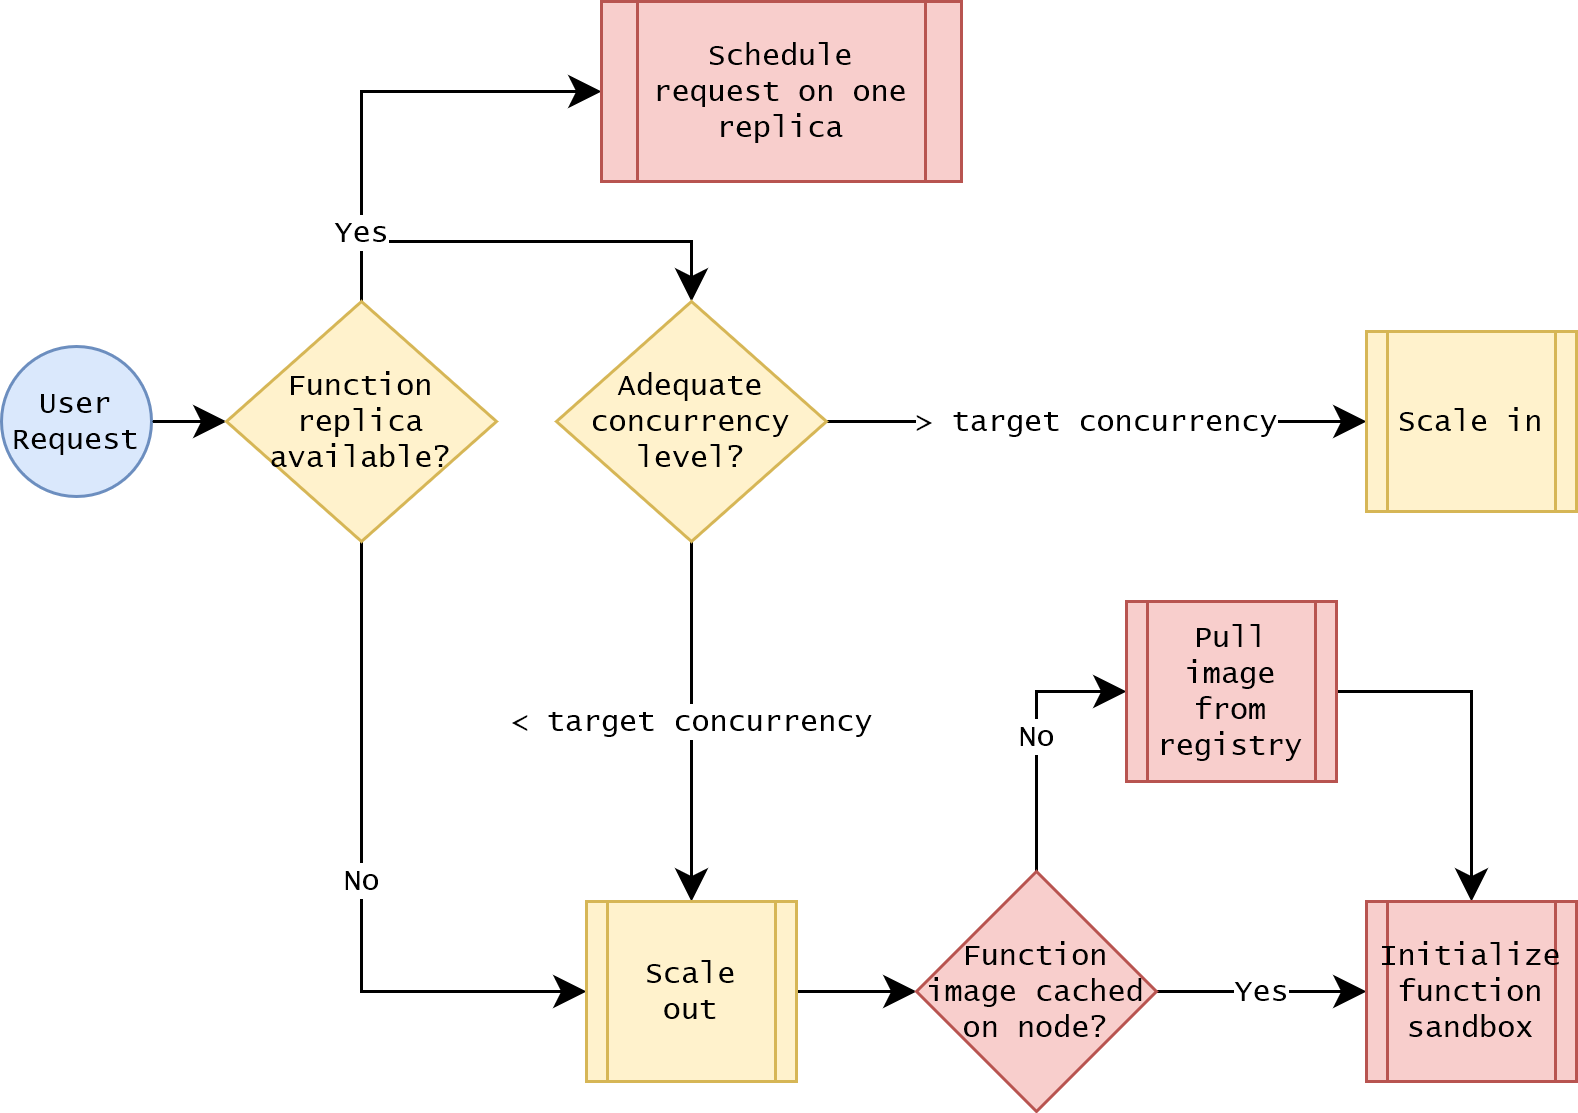
\includegraphics[width=0.8\columnwidth]{6_Chapitre4/figures/function-cache.png}
\caption{Lifecycle of a user request in a serverless platform.}
\label{figure:herocache-function-cache}
\end{figure}

\begin{figure}[t]
\centering
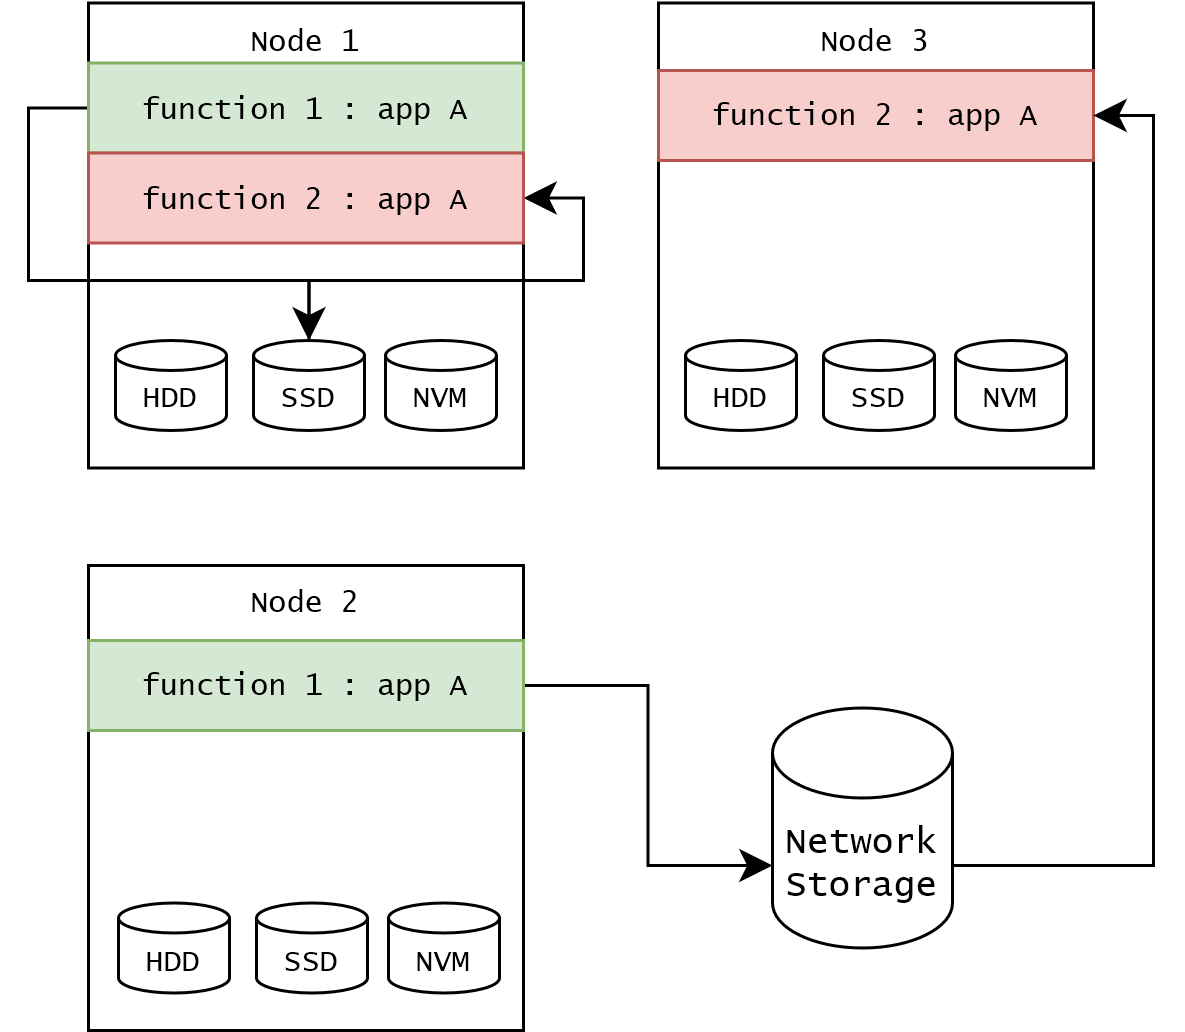
\includegraphics[width=0.8\columnwidth]{6_Chapitre4/figures/function-communications.png}
\caption{Serverless functions communicate intermediate results through persistent storage that can be local to edge nodes or remotely accessible.}
\label{figure:herocache-function-communications}
\end{figure}

\begin{figure*}[t]
\centering
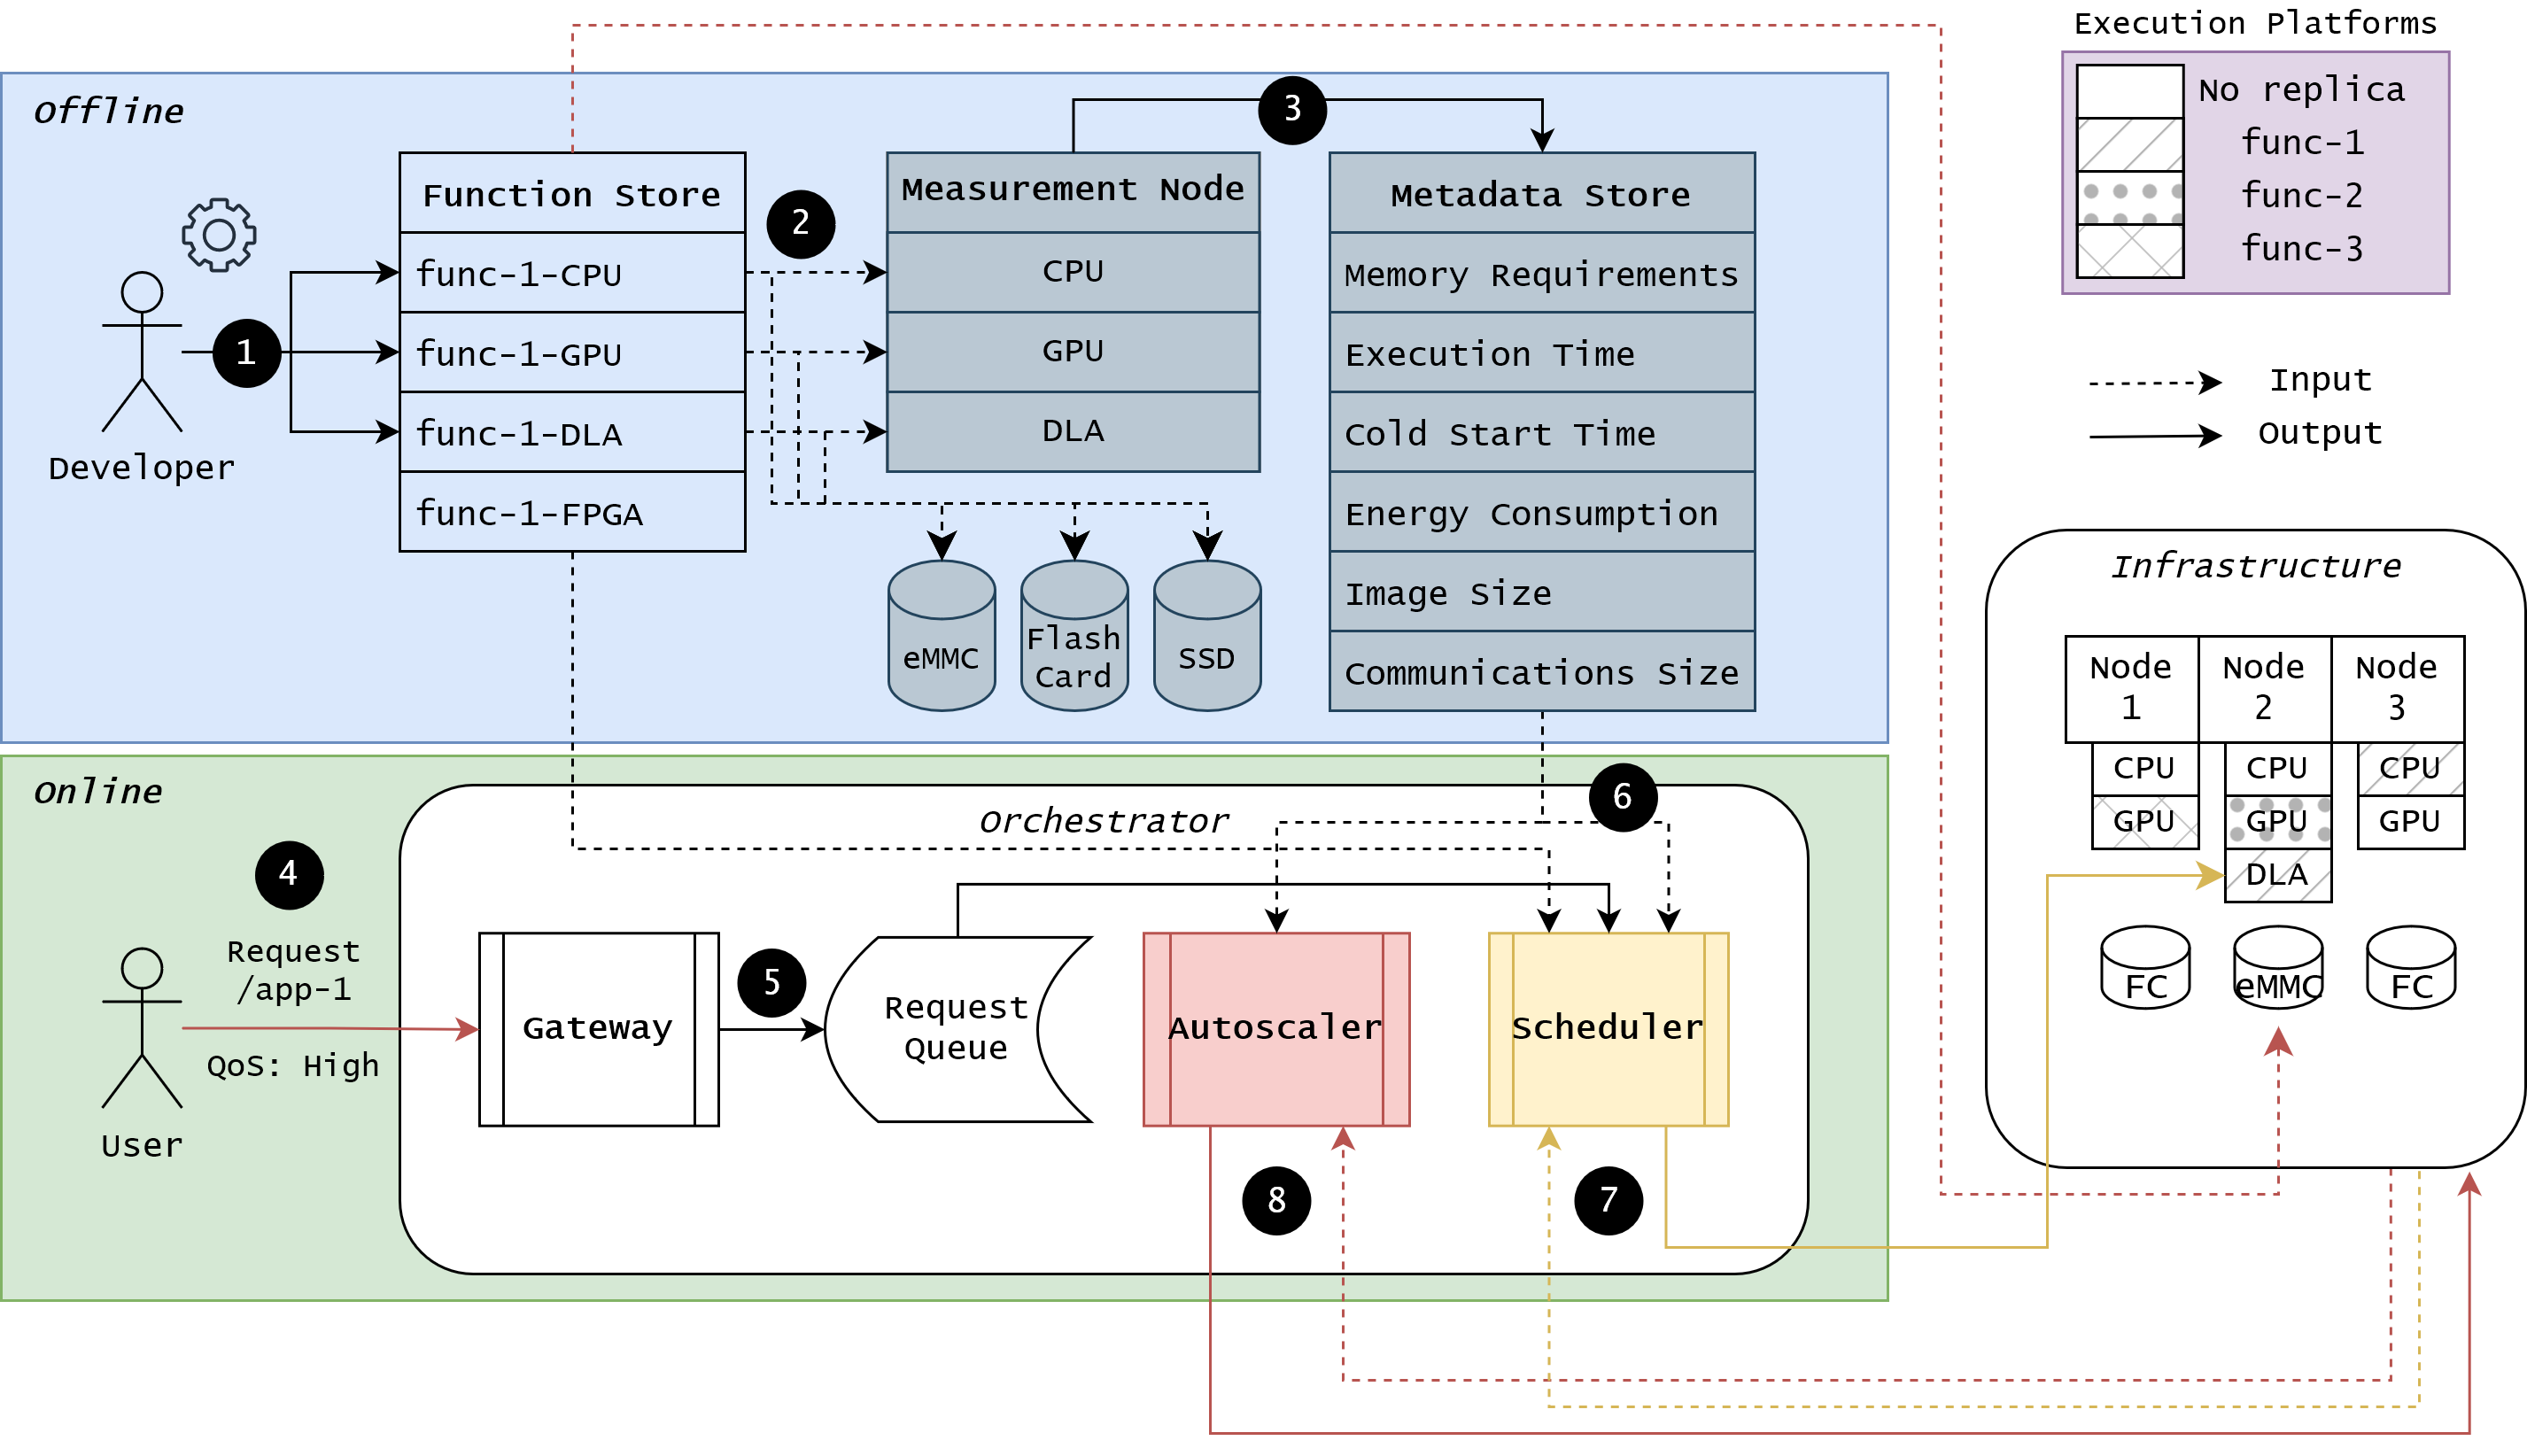
\includegraphics[width=0.65\textwidth]{6_Chapitre4/figures/serverless-platform-storage.png}
\caption{Serverless IDS platform, system overview}
\label{figure:herocache-serverless-platform}
\end{figure*}

\subsection{Défis de l'orchestration dynamique}

Le serverless est un modèle de service tendance pour le cloud~\cite{Lannurien2023} : en transférant la responsabilité de l'allocation des ressources des clients aux fournisseurs de services, il allège une partie importante de la complexité des développeurs d'applications et ouvre de nouvelles possibilités d'optimisation et de contrôle des coûts pour le gestionnaire d'infrastructure.
Dans une architecture serverless, les développeurs conçoivent leurs applications comme une composition de fonctions sans état. Sans état (ou "pur", sans effet secondaire) signifie que le résultat du calcul dépend exclusivement des entrées \cite{burckhardtNetheriteEfficientExecution}. Ces fonctions prennent en entrée une charge utile et un contexte d'invocation, et produisent un résultat qui est stocké dans un niveau de stockage persistant accessible par le réseau. Cela signifie que les dépendances de données entre les fonctions d'une chaîne doivent être gérées par la plateforme.

Lorsqu'un événement déclenche leur exécution, les fonctions sont déployées sur des nœuds de l'infrastructure, dans des environnements d'exécution appelés \textbf{répliques}. Comme les fonctions sont sans état, les demandes peuvent être attribuées à n'importe quelle réplique disponible. La mise à l'échelle d'une application serverless, \textit{i.e.} pour maintenir un niveau de performance constant, consiste à faire croître ou décroître le pool de répliques des fonctions en suivant les pics de charge. Les plateformes serverless basées sur Kubernetes, telles que Knative \cite{knative} ou OpenWhisk \cite{openwhisk}, ont proposé un modèle basé sur le seuil pour le rightsizing du pool de réplicas. Pour toute fonction, un \textit{autoscaler} peut déployer plusieurs \textit{répliques} pour absorber la charge. Chaque réplique est allouée à une plateforme d'exécution (\textit{e.} un cœur de CPU, un GPU, etc.) et dispose d'une file d'attente de longueur fixe pour les demandes entrantes. Le nombre de répliques pour une fonction donnée à un moment donné détermine son niveau de concurrence. Un ordonnanceur place les demandes des utilisateurs dans la file d'attente des répliques de la fonction. Lorsqu'une réplique n'a plus de demandes, elle est désattribuée. Lorsqu'une fonction est demandée alors qu'aucune réplique n'existe, elle passe par un \textbf{démarrage à froid} qui entraîne un délai d'initialisation du temps de réponse de la fonction.

Dans le serverless, la fréquence des allocations de ressources augmente considérablement par rapport aux environnements à ressources réservées toujours actives, tels que les offres IaaS. La capacité des plateformes serverless à mettre à l'échelle une fonction jusqu'à zéro réplique afin d'éviter de facturer les clients pour des ressources inactives est une différence essentielle par rapport aux modèles de services cloud traditionnels.

Ce démarrage à froid présente un risque d'augmentation de la latence, car le fournisseur doit allouer des ressources matérielles et instancier l'application avant de répondre à la demande. Plus l'application est complexe, plus le risque de retards importants est élevé~\cite{mohanAgileColdStartsa}. Les fournisseurs pré-affectent généralement certaines ressources pour éviter les démarrages à froid, ce qui a un coût en termes de provisionnement des ressources. Les acteurs commerciaux tels qu'AWS, Google et Microsoft réutilisent tous, dans une certaine mesure, des instances de fonction, en les laissant fonctionner pendant une période de temporisation afin de contourner les coûts de latence induits par les démarrages à froid~\cite{vahidiniaColdStartServerless2020}.

Une étude récente a montré que 50\% des applications serverless déployées sur Microsoft Azure Durable Functions \footnote{\href{https://learn.microsoft.com/en-US/azure/azure-functions/durable/durable-functions-overview}{https://learn.microsoft.com/en-US/azure/azure-functions/durable/durable-functions-overview}} sont constituées de 3 fonctions ou moins, 65\% des applications présentant un simple DAG de fonctions agencées sous forme de chaînes linéaires \cite{mahgoubORIONThreeRights}. Notre application IDS se compose de différentes chaînes de deux fonctions, comme décrit dans la section~\ref{section:herocache-characterization-workloads}. Les travaux de caractérisation des charges de travail ont montré que 25\% des fonctions déployées sur Microsoft Azure Functions \footnote{\href{https://azure.microsoft.com/en-us/products/functions/}{https://azure.microsoft.com/en-us/products/functions/}} s'exécutent en 100 ms ou moins \cite{shahradServerlessWildCharacterizing}. Les fonctions qui composent notre application IDS s'exécutent pendant des centièmes ou des dixièmes de seconde, ce qui les rend particulièrement sujettes à des ralentissements critiques dans le contexte de ressources allouées de manière dynamique.

\subsection{Mise en cache des images de fonctions}
\label{section:herocache-background-cache}

En ligne, l'allocation dynamique des ressources et les politiques de placement des tâches peuvent aider à répondre aux exigences de qualité de service (QoS) par demande en attribuant les requêtes aux répliques appropriées dans l'infrastructure. Cependant, la plupart des articles sur l'orchestration des ressources et le placement des tâches dans le serverless ne considèrent que les meilleurs scénarios, dans lesquels les images de fonctions sont déjà disponibles sur les nœuds edge. Cela ne reflète pas la réalité, où les images de fonctions sont stockées dans des registres sur des nœuds dédiés et téléchargées sur les nœuds de calcul lors du déploiement des fonctions. En fonction de la taille de l'image, cela peut avoir des conséquences néfastes sur la latence des requêtes avec des déploiements où les démarrages à froid dominent le temps de réponse total d'une fonction \cite{yanHermesEfficientCache2020}.

Afin de répondre aux demandes des utilisateurs sans dégrader les performances, l'autoscaler ajuste périodiquement le nombre de répliques pour chaque fonction déployée : le pool de répliques croît et décroît en fonction des variations de la charge de l'application. Lorsque la charge d'une fonction augmente au-delà du seuil de concurrence de la plateforme, l'autoscaler crée une nouvelle réplique qui traitera les demandes supplémentaires des utilisateurs. Lorsque la charge diminue, les répliques inactives sont supprimées. S'il n'y a plus de demandes pour une fonction donnée, celle-ci peut être \textit{scaled to zero}, ce qui permet d'éviter le gaspillage des ressources.

Les répliques de fonctions sont initialisées à partir d'\textbf{images de fonctions} (\textit{e.g.} une image Docker). Celles-ci sont stockées dans un registre d'images. Ces registres peuvent être accessibles à distance via l'internet et sont généralement déployés dans l'infrastructure du fournisseur dans le contexte d'un nuage privé. Toutefois, de nombreuses études antérieures \cite{bhasiCypressInputSizesensitive2022, zijunFassflowEfficient2022, smithFaDOFaaSFunctions2022, zhangFIRSTExploitingMultiDimensional2023} n'envisagent que des scénarios optimaux dans lesquels les images de fonctions sont déjà disponibles sur les nœuds edge. Cela ne reflète pas la réalité où les images de fonctions sont stockées dans des registres sur des nœuds dédiés et tirées par les nœuds de bordure où et quand les fonctions sont déployées. En fonction de la taille de l'image, cela peut avoir des conséquences néfastes sur la latence des requêtes, en particulier dans les cas où les démarrages à froid dominent le temps de réponse total d'une fonction.

En fait, l'extraction d'images sur les nœuds edge peut représenter plus de 80\% du temps de réponse d'une fonction \cite{yanHermesEfficientCache2020} puisque la latence du démarrage à froid domine le temps de réponse total de la fonction. Cette situation n'est pas acceptable lorsque la plateforme doit répondre à des exigences strictes en matière de qualité de service, comme c'est le cas pour les tâches critiques telles que l'IDS.

\subsection{Communications entre les fonctions}
\label{section:herocache-background-communications}

En outre, comme ces fonctions sont parfois mises à l'échelle à partir de zéro, elles ne sont pas adressables par le réseau : les communications entre les fonctions sont réalisées par l'utilisation d'un stockage lent et accessible par le réseau (\textit{e.g.} Amazon S3). Cela induit des retards qui peuvent faire boule de neige tout au long de l'exécution de l'application et provoquer des violations de l'objectif de niveau de service (SLO) en augmentant les latences de queue de requête \cite{wawrzoniakBoxerDataAnalytics2021a}. Les offres FaaS sont un exemple typique d'architecture d'expédition de données : des gigaoctets de données sont déplacés vers des mégaoctets de code, ce qui entraîne des inefficacités qui augmentent la consommation d'énergie et la sous-utilisation des ressources.

Comme il est nécessaire de prendre en charge la mise à l'échelle dynamique des fonctions, chaque invocation d'une fonction serverless est autonome et ne porte pas les informations ou le contexte des invocations précédentes. Cela permet aux répliques de mettre en file d'attente les demandes des utilisateurs et de les traiter de manière séquentielle sans avoir besoin de procéder à un démarrage à froid entre les demandes. Cela introduit une contrainte sur la plateforme serverless : si une application est composée de plusieurs fonctions qui forment un pipeline de traitement, la sortie de chaque fonction doit être stockée dans un stockage persistant pour être alimentée en entrée de la fonction suivante dans la chaîne~\cite{mullerLambadaInteractiveData2020}.

Les travaux de l'état de l'art ont montré que les fonctions serverless qui communiquent par le biais d'un stockage distant peuvent subir un ralentissement jusqu'à 11x par rapport aux fonctions utilisant des communications directes \cite{wawrzoniakBoxerDataAnalytics2021a}. Les fonctions de notre application IDS doivent communiquer des résultats intermédiaires à chaque étape du DAG de l'application. Lorsque les fonctions sont déployées sur différents nœuds edge, les communications inter-fonctions devront être réalisées par l'utilisation d'un stockage à distance. Cela introduit des ralentissements qui peuvent faire boule de neige tout au long de l'exécution des fonctions et détériorer la qualité de service de l'ensemble de l'application.

\section{Détection d'intrusion à l'edge dans le modèle serverless}
\label{section:herocache-before-contrib}

Orchestrer des applications serverless tout en atteignant le SLA nécessite de modéliser soigneusement les caractéristiques de l'application et d'en tenir compte lors de l'allocation des ressources et de l'ordonnancement des demandes des utilisateurs sur la plateforme serverless. La figure~\ref{figure:herocache-serverless-platform} donne un aperçu du cycle de vie global d'une requête sur notre plateforme serverless. Il est divisé en deux phases ; une \textbf{phase hors-ligne} qui consiste à caractériser les applications déployées par les utilisateurs sur les plateformes edge, et une \textbf{phase en ligne} où les requêtes vers ces applications sont ordonnancées sur la plateforme.

\textbf{phase hors-ligne}. Dans notre plateforme, le cycle de vie de l'application commence par une phase hors-ligne, au cours de laquelle le développeur fournit le code de ses fonctions pour différentes architectures matérielles (GPU, CPU, DLA, etc.)~\Circled{1}. Ce code est stocké par le fournisseur de services dans un registre de fonctions. Les fonctions sont ensuite déployées sur un nœud de mesure~\Circled{2} où elles sont exécutées pour générer des métadonnées relatives à l'exécution des fonctions sur des nœuds hétérogènes. Les besoins en mémoire, le temps d'exécution, le temps de démarrage à froid, la consommation d'énergie, la taille de la fonction et la taille de la communication pour chaque fonction sont enregistrés dans un magasin de métadonnées~\Circled{3}. L'exécution de la phase hors-ligne est nécessaire une fois pour une fonction donnée sur une plateforme donnée, comme décrit dans la section~\ref{section:herocache-workload}.

\textbf{Phase en ligne}. Les demandes sont envoyées aux applications IDS avec une charge utile de trafic TCP (paquets sérialisés) à analyser~\Circled{4}, et un niveau de qualité de service souhaité associé pour le temps de réponse de la demande. La demande est ajoutée à une file d'attente~\Circled{5} au niveau de l'orchestrateur. Lorsque l'ordonnanceur extrait la demande de la file d'attente, le magasin de métadonnées est interrogé pour récupérer les métadonnées de fonction appropriées~\Circled{6}.

L'ordonnanceur tente alors de trouver une réplique disponible de la première fonction de l'application pour traiter la demande~\Circled{7}. Si une telle réplique n'existe pas encore, il sera demandé à l'autoscaler d'initialiser une nouvelle instance de la fonction~\Circled{8}. Au cours du cycle de vie de l'application, l'autoscaler vérifie périodiquement la charge moyenne de chaque fonction pour ajuster le nombre de répliques déployées sur la plateforme, en fonction du seuil de concurrence fixé par le fournisseur de services.

Lorsque l'application est terminée, elle renvoie à l'utilisateur un vecteur de classification qui indique les probabilités que le trafic soit malveillant, c'est-à-dire qu'il présente les caractéristiques d'une attaque potentielle.

\section{Phase hors-ligne : caractérisation} 
\label{section:herocache-workload}

\begin{figure}[t]
\centering
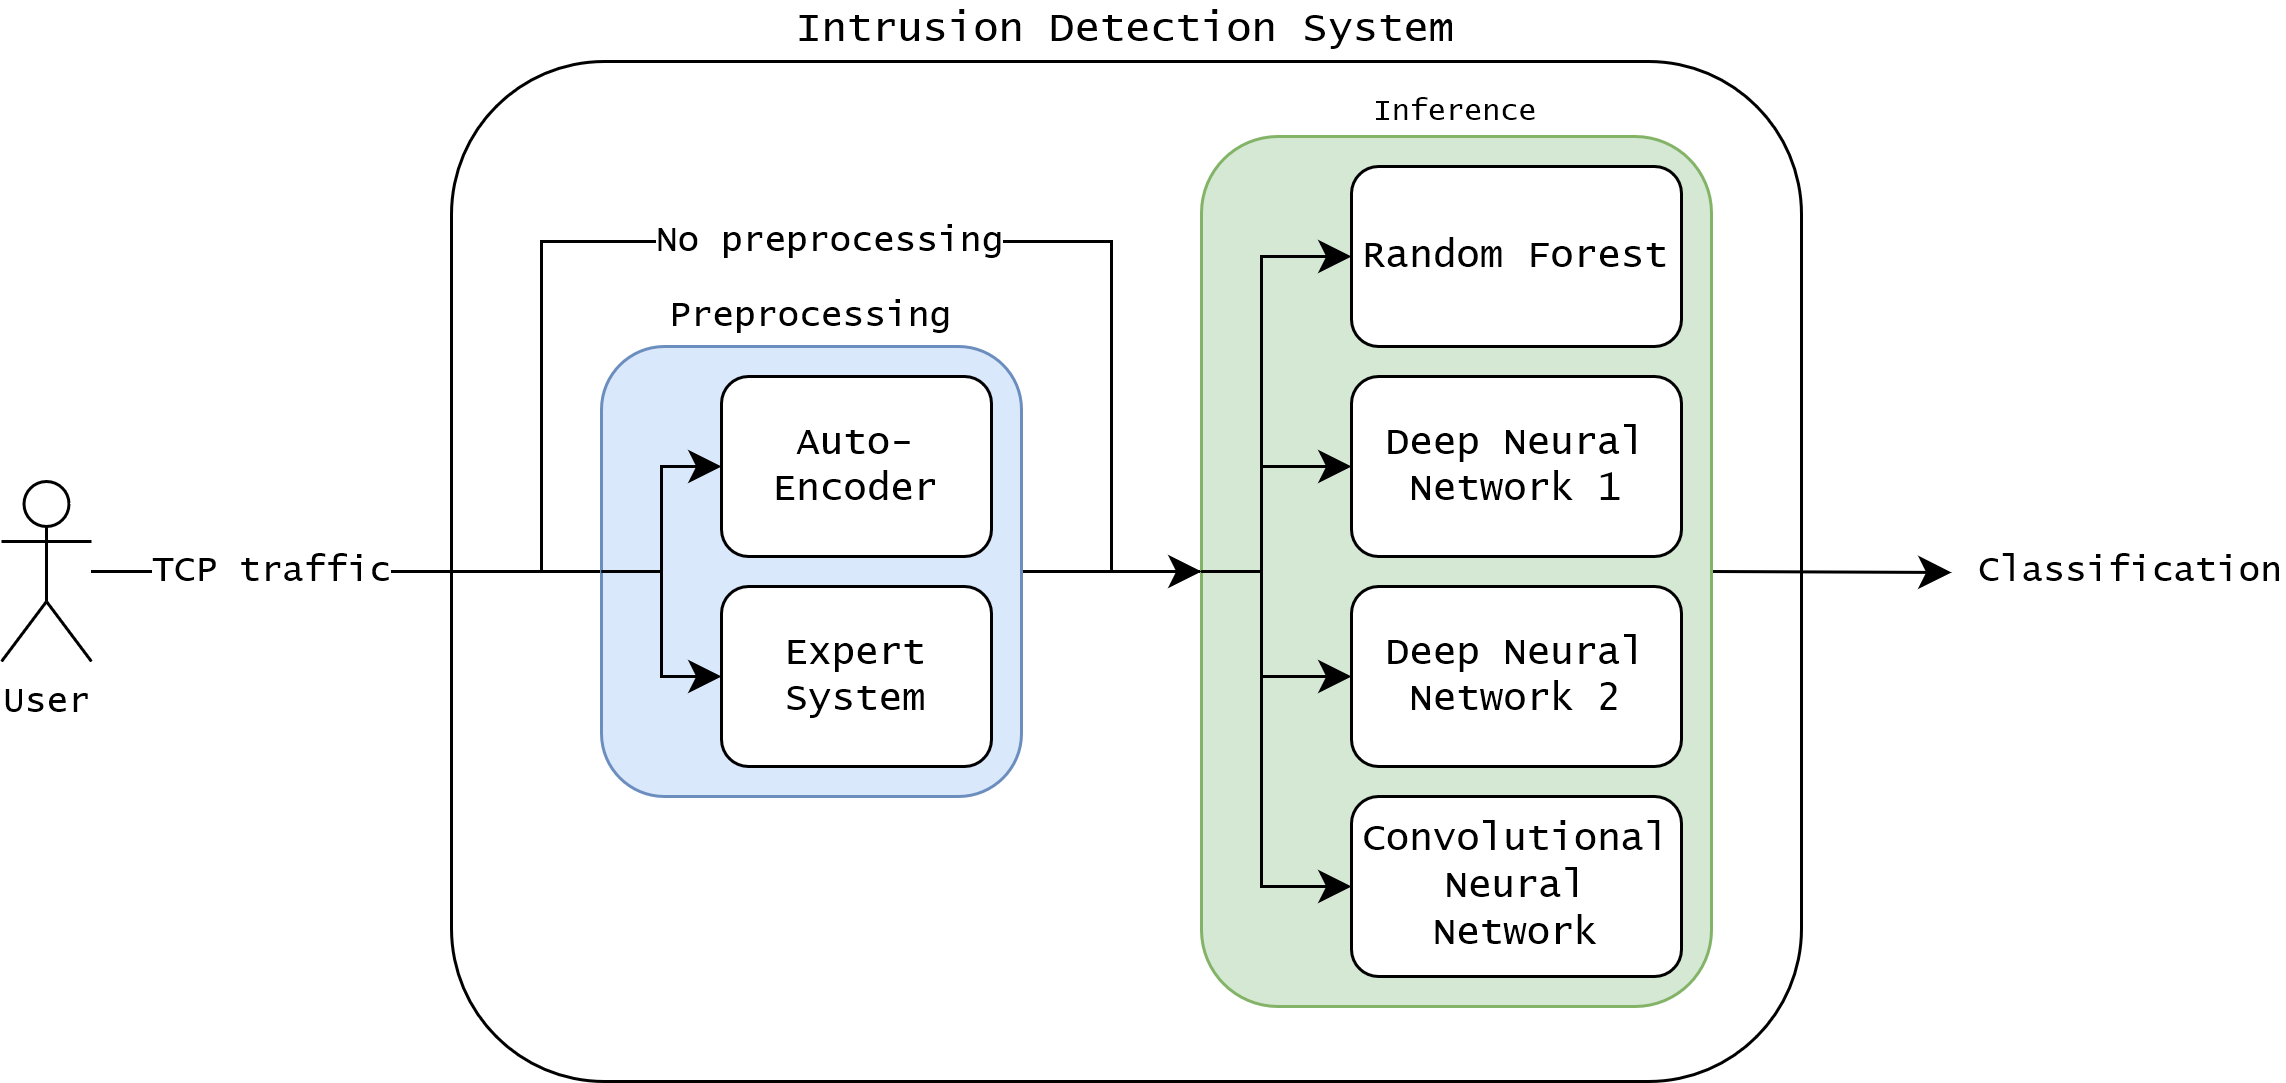
\includegraphics[width=0.8\columnwidth]{6_Chapitre4/figures/ids-application.png}
\caption{Architecture of an IDS application that can make use of different preprocessing functions, and different inference functions to provide the user with a classification of TCP traffic.}
\label{figure:herocache-ids-application}
\end{figure}

Une étape préliminaire de caractérisation de la plateforme et de la charge de travail est nécessaire pour parvenir à une allocation des ressources et à un placement des tâches adéquats pour l'exécution des modèles IDS. À cette fin, nous avons évalué plusieurs modèles IDS en termes de performance et d'énergie sur des plates-formes hétérogènes représentatives des dispositifs edge~\cite{kljucaric2020}. Ces mesures sont cruciales pour une orchestration efficace sur des plates-formes hétérogènes à l'edge. Cette section décrit notre méthodologie et nos résultats.

\subsection{Caractérisation des plateformes d'exécution} \label{section:herocache-characterization-platforms}

Nous avons utilisé des plateformes représentatives de ce que l'on peut trouver en bordure~\cite{slimani:hal-04159551,kljucaric2020} : 
 Il fonctionne sous Linux Raspbian 5.4.
\textbf{(2) Nvidia Jetson Xavier AGX} composé de trois éléments de traitement : un CPU NVIDIA ARM Carmel à 8 cœurs, un GPU NVIDIA Volta avec 512 cœurs CUDA et un accélérateur d'apprentissage profond (DLA), qui est un accélérateur matériel à fonction fixe conçu pour les réseaux neuronaux convolutifs (CNN). Il est supposé être plus économe en énergie que le GPU. Le NVIDIA Xavier AGX est équipé de 16 Go de mémoire LPDDR4 et de 32 Go de mémoire flash eMMC 5.1. Il fonctionne sous Linux Tegra 4.9.10. Le mode d'alimentation 15 Watts Desktop a été utilisé. 
\textbf{(3) PYNQ-Z2 Development Board}, une carte basée sur le système sur puce Xilinx Zynq XC7Z020. Elle est équipée d'un FPGA Artix-7, d'une mémoire DDR3 de 512 Mo et d'une carte SD de 16 Go.

\subsection{Caractérisation des applications}
\label{section:herocache-characterization-workloads}

Notre application se compose de différents préprocesseurs et classificateurs. Le préprocesseur sélectionne un sous-ensemble de caractéristiques pertinentes des paquets TCP. 3 approches de prétraitement différentes ont été utilisées : (1) utilisation de toutes les caractéristiques des paquets sans aucune sélection (NoFS : No Feature Selection) ; (2) utilisation d'un auto-encodeur DNN pour projeter les caractéristiques dans un espace latent plus petit (AE : Auto-Encoder) ; et (3) sélection experte d'un sous-ensemble de caractéristiques (ES : Expert Selection). Pour la partie classification, nous avons utilisé Random Forest (RF), deux architectures différentes de réseaux neuronaux denses (DNN) et un CNN.

\begin{table}[t]
\caption{IDS models architectures and sizes}
\resizebox{\textwidth}{!}{
\begin{tabular}{|c|c|cc|}
\hline
Model     & Architecture                                                                                                                                         & \multicolumn{1}{c|}{Model Size on CPUs (MB)} & Model Size on GPU (MB) \\ \hline
NoFS-RF   & \begin{tabular}[c]{@{}c@{}}5 trees of 100\\ maximum depth\end{tabular}                                                                               & \multicolumn{1}{c|}{28}                      & 15.4                   \\ \hline
AE-RF     & \begin{tabular}[c]{@{}c@{}}5 trees of 50 \\ maximum depth\end{tabular}                                                                               & \multicolumn{1}{c|}{-}                       & 32.9                   \\ \hline
ES-RF     & \begin{tabular}[c]{@{}c@{}}10 trees of 10 \\ maximum depth\end{tabular}                                                                              & \multicolumn{1}{c|}{9.1}                     & 5.5                    \\ \hline
NoFS-DNN1 & \multirow{3}{*}{\begin{tabular}[c]{@{}c@{}}4 Dense Layers \\ (128x64x32x10)\end{tabular}}                                                            & \multicolumn{2}{c|}{0.144}                                            \\ \cline{1-1} \cline{3-4} 
AE-DNN1   &                                                                                                                                                      & \multicolumn{2}{c|}{0.321}                                            \\ \cline{1-1} \cline{3-4} 
ES-DNN1   &                                                                                                                                                      & \multicolumn{2}{c|}{0.053}                                            \\ \hline
NoFS-DNN2 & \multirow{3}{*}{\begin{tabular}[c]{@{}c@{}}5 Dense Layers \\ (7024x704x288x64x10)\end{tabular}}                                                      & \multicolumn{2}{c|}{3.33}                                             \\ \cline{1-1} \cline{3-4} 
AE-DNN2   &                                                                                                                                                      & \multicolumn{2}{c|}{2.96}                                             \\ \cline{1-1} \cline{3-4} 
ES-DNN2   &                                                                                                                                                      & \multicolumn{2}{c|}{2.61}                                             \\ \hline
NoFS-CNN  & \multirow{3}{*}{\begin{tabular}[c]{@{}c@{}}2 Conv1D (x64) - MaxPool \\ 3 Conv1D (x256) - MaxPool\\ 3 Dense Layers (100x20x10)\end{tabular}} & \multicolumn{2}{c|}{4.77}                                             \\ \cline{1-1} \cline{3-4} 
AE-CNN    &                                                                                                                                                      & \multicolumn{2}{c|}{2.9}                                              \\ \cline{1-1} \cline{3-4} 
ES-CNN    &                                                                                                                                                      & \multicolumn{2}{c|}{2.6}                                              \\ \hline
\end{tabular}
}
\label{table:herocache-workload}
\end{table}

Le tableau~\ref{table:herocache-workload} présente les modèles IDS pris en compte dans cette étude et certaines de leurs caractéristiques. Ces modèles ont été formés et caractérisés sur l'ensemble de données de référence sur les intrusions dans le réseau UNSW-NB15\footnote{\href{https://research.unsw.edu.au/projects/unsw-nb15-dataset}{https://research.unsw.edu.au/projects/unsw-nb15-dataset}}
où chaque observation représente des caractéristiques statistiques, de contenu et de temps sur le trafic de données au cours d'une fenêtre temporelle, et est étiquetée comme "normale" ou "attaque". L'ensemble de données comprend 9 catégories d'attaques. Les modèles de réseaux neuronaux ont été exportés et optimisés à l'aide de TensorFlow Lite et TensorRT lorsqu'ils étaient destinés à des plateformes CPU et GPU/DLA, respectivement. En ce qui concerne Random Forest, les modèles ont été exportés en utilisant les frameworks Emlearn et HummingBird.ml lorsqu'ils étaient destinés aux plateformes CPU et GPU, respectivement. hls4ml a été utilisé pour exporter les modèles de réseaux neuronaux pour la cible FPGA.

\subsection{Mesures de performances}

Chacun des modèles IDS a été déployé sur les plateformes cibles et les inférences ont été exécutées avec un ensemble de 80 000 paquets provenant de l'ensemble de données UNSW-NB15 afin de caractériser la latence d'inférence. Les résultats sont présentés dans la figure~\ref{figure:herocache-performance}. Seul un modèle (ES-DNN1) a été caractérisé sur la plateforme FPGA car les autres modèles HLS n'ont pas pu être pris en compte sur la cible. La conclusion qui a été tirée de ces résultats est que pour les réseaux neuronaux, le CPU Xavier atteint la meilleure performance dans la majorité des cas, à l'exception de NoFS-CNN qui profite des capacités du GPU en raison de son nombre élevé de paramètres et de l'efficacité du GPU pour les opérations de convolution. Pour les modèles Random Forest, l'élément de traitement le plus rapide est le GPU. En termes de coût et de disponibilité, la Xavier AGX est respectivement environ 20x et 10x plus chère que les plateformes RBPI4 et Pynq-Z2. Nous dimensionnons notre infrastructure en conséquence en fournissant plus de plateformes RBPI4 que de Xavier AGX pour être représentatifs des déploiements réels.

\begin{figure}
    \centering
    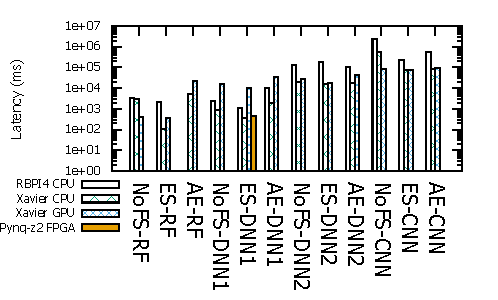
\includegraphics[width=0.9\columnwidth]{6_Chapitre4/figures/latency_bar.pdf}
    \caption{Latency characterization of IDS models.}
    \label{figure:herocache-performance}
\end{figure}

\subsection{Mesures de consommation d'énergie}

Nous avons exécuté des inférences sur les modèles IDS sur chaque élément de traitement et mesuré la consommation d'énergie de la plateforme à l'aide de l'analyseur de puissance N6705A DC. Les résultats sont présentés dans la figure~\ref{figure:herocache-energy}. Pour les mêmes raisons que celles mentionnées ci-dessus, seul ES-DNN1 a été caractérisé sur FPGA. Nous observons que les éléments de traitement du CPU affichent une consommation d'énergie inférieure à celle du GPU dans la majorité des cas. Le seul cas où le GPU obtient de meilleurs résultats est lorsque la vitesse qu'il atteint par rapport aux CPU est élevée. C'est par exemple le cas pour NoFS-CNN, où le CPU RBPI4 est plus de 30 fois plus lent que le GPU. Même si Pynq-Z2 présente la meilleure efficacité énergétique avec le modèle ES-DNN1, étant donné qu'il est plus cher et présente une générosité de conception limitée, nous supposons qu'il est moins disponible que le RBPI4.

\begin{figure}
    \centering
    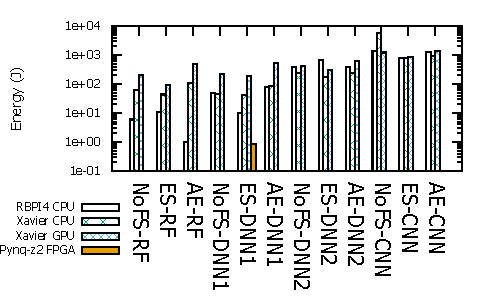
\includegraphics[width=0.9\columnwidth]{6_Chapitre4/figures/energy_bar.pdf}
    \caption{Energy characterization of IDS models.}
    \label{figure:herocache-energy}
\end{figure}

\section{Phase en ligne : orchestration avec HeROcache} \label{section:herocache-contribution}

\subsection{Présentation générale}

L'orchestrateur HeROcache est principalement composé de deux modules, le \textbf{autoscaler} et le \textbf{scheduler} (voir figure~\ref{figure:herocache-serverless-platform}). L'autoscaler est chargé de l'allocation dynamique des ressources : il affecte les plateformes d'exécution aux répliques de fonctions. L'ordonnanceur s'occupe du placement des demandes des utilisateurs sur les répliques.

HeROcache relève les trois défis susmentionnés en concevant des stratégies complémentaires de minimisation des coûts au niveau de l'autoscaler et de l'ordonnanceur. HeROcache minimise \textbf{les délais d'initialisation} en tenant compte des temps de latence de l'extraction d'images au niveau de l'autoscaler. Des stratégies d'extraction préalable sont également mises en œuvre pour la mise en cache des images de fonctions. Les coûts de \textbf{communication interfonction} sont pris en compte principalement dans la partie de l'ordonnanceur, qui tend naturellement à consolider les fonctions d'une même application. L'autoscaler participe indirectement à cette consolidation en préemptant les fonctions suivantes du DAG de l'application sur le même nœud de bordure. Enfin, \textbf{plateformes hétérogènes} sont prises en compte car les différents coûts d'exécution extraits pendant la phase hors-ligne (voir Section~\ref{section:herocache-workload}) sont pris en compte tout au long du processus d'autoscaling et d'ordonnanceur. Les sections suivantes décrivent les stratégies de mise à l'échelle automatique et d'ordonnanceur.

\begin{table}[t]
    \caption{Notation dictionary}
    \begin{center}
    \scalebox{0.85}{\begin{tabularx}{\linewidth}{|c|Y|}
    \hline
    \textbf{Notation} & \textbf{Description} \\ \hline
    $x_a$ & Allocation of resource for application $a$ \\ \hline
    $y_a$ & Invocation of application $a$ \\ \hline
    $z_i$ & Placement of task for function $i$ \\ \hline
    $f_{N, P}$ & A function $f$ scheduled to run on a platform $P$ available on node $N$ \\ \hline
    $f_{a}$ & A function $f$ that belongs to application $a$ \\ \hline
    $A$ & Total number of applications to be scheduled on the platform \\ \hline
    $F_{a}$ & Total number of functions that belong to an application $a$ \\ \hline
    $RT_{{f}_{N, P}}$ & Time to retrieve function image for $f$ to run on a platform $P$ available on node $N$ \\ \hline
    $NB_{N}$ & Network bandwidth between node $N$ and the infrastructure \\ \hline
    $SMT_{N}$ & Storage medium throughput on node $N$ \\ \hline
    $SML_{N}$ & Storage medium latency on node $N$ \\ \hline
    $QP$ & QoS penalty \\ \hline
    $QD$ & QoS deviation \\ \hline
    $WET$ & Worst execution time \\ \hline
    $TT$ & Task total time \\ \hline
    $CST$ & Cold start time \\ \hline
    $ST$ & Storage time \\ \hline
    $ET$ & Execution time \\ \hline
    $EC$ & Energy consumption \\ \hline
    $IS$ & Image size \\ \hline
    $HP$ & Hardware price \\ \hline
    $TC$ & Task consolidation \\ \hline
    $Q$ & Task queue on a replica \\ \hline
    $CP$ & Cache proportion \\ \hline
    $SIS^{f}_{a}$, $SOS^{f}_{a}$ & Size of resp. input, output state of function $f$ that belongs to application $a$ \\ \hline
    $threshold_{f, h}$ & Concurrency threshold for a function $f$ on a replica of hardware type $h$ \\ \hline
    $scaleCost^{{f}_{{i}_{N, P}}}_a$ & Cost of creating a new replica for function $f_i$ from application $a$ on a platform $P$ available on node $N$ \\ \hline
    $schedCost^{{f}_{{i}_{N, P}}}_a$ & Cost of scheduling an execution of function $f$ from application $a$ on a platform $P$ available on node $N$ \\ \hline
    \end{tabularx}}
    \label{table:herocache-notation}
    \end{center}
\end{table}

\subsection{Stratégie de minimisation des coûts d'allocation des ressources}

Nous formulons l'allocation des ressources comme un problème d'optimisation et nous le résolvons à l'aide d'un algorithme gourmand simple. L'objectif de l'autoscaler est de minimiser le coût de la somme des allocations $scaleCost_{a}$ pour $y_a$ invocations de l'application $a$ (équation~\ref{eq:herocache-objective-allocation}) pour toutes les applications dans $A$, sous la contrainte d'une infrastructure finie avec $x_a$ étant l'allocation de ressources pour l'application $a$ (équation~\ref{eq:herocache-constraint-allocation}). 

\begin{equation}
    \forall A, \, \min \sum_{a = 0}^{A} y_a \cdot scaleCost_{a}
\label{eq:herocache-objective-allocation}
\end{equation}

\begin{equation}
    \text{s. t.} \, \sum_{a = 0}^{A} x_a \leq Total Resources
\label{eq:herocache-constraint-allocation}
\end{equation}

Le coût de l'allocation des ressources pour une application $a$ est la somme des coûts d'allocation de ses fonctions (équation~\ref{eq:herocache-scale-cost-app}). Une réplique est allouée à une plateforme d'exécution.

\begin{equation}
    scaleCost_{a} = \, \sum_{i = 0}^{F_{a}} scaleCost^{{f}_{{i}_{N, P}}}_a
\label{eq:herocache-scale-cost-app}
\end{equation}

Chaque réplique de fonction a un coût d'allocation associé, car l'allocation dynamique des ressources matérielles introduit un temps de latence lors du traitement des demandes des utilisateurs. 

Nous avons conçu un modèle de coût (équation~\ref{eq:herocache-scale-cost-function}) pour l'allocation des ressources nécessaires au déploiement d'une fonction d'une application donnée. Il est composé de quatre éléments, dont nous devons minimiser la somme :

\begin{itemize}
    \item La \textit{proportion de cache} $CP$ traduit la dispersion des fonctions sur les différents nœuds de bordure. Plus le score est élevé, plus les fonctions sont dispersées sur les nœuds. La minimisation de ce terme permet de consolider les fonctions ;
    \item Le \textit{temps total} $TT$ représente le temps d'exécution total de la fonction. Il tient compte de la qualité de service de l'application, de l'hétérogénéité de la plateforme et du coût de déploiement (si l'image est mise en cache ou distante). Plus ce coût est élevé, plus la qualité de service est faible ;
    \item La \textit{consommation d'énergie} $EC$ traduit la consommation d'énergie du déploiement de la fonction. Plus $EC$ est élevé, plus le coût est important ;
    \item Le \textit{prix du matériel} $HP$ décrit le coût total de possession (TCO) supporté par les fournisseurs de services en fonction du temps d'exécution. Il traduit le coût de déploiement sur une plateforme matérielle donnée. Plus $HP$ est élevé, plus le coût de la solution est important.
\end{itemize}

L'objectif global du modèle de coût est de déployer une fonction au coût le plus bas possible, c'est-à-dire une consolidation accrue, une réduction du makespan, une réduction de la consommation d'énergie et une réduction du coût de possession. Nous détaillerons chaque partie de l'équation~\ref{eq:herocache-scale-cost-function} dans les paragraphes suivants. Chaque composante de l'équation est pondérée pour permettre un réglage souple ; les valeurs que nous avons choisies pour le déploiement de l'application IDS sont spécifiées dans la partie consacrée à l'évaluation (Section~\ref{section:herocache-evaluation}).

\begin{equation}
\begin{split}
 \forall N, \forall P \in N, scaleCost^{{f}_{{i}_{N, P}}}_{a} = \,   &k_{CP} \cdot {CP}_{{a}_{N}}    \\
    + &k_{TT} \cdot {TT}_{{f}_{N, P}} \\
    + &k_{EC} \cdot {EC}_{{f}_{N, P}} \\
    + &k_{HP} \cdot {HP}_{{f}_{N, P}}
\end{split}
\label{eq:herocache-scale-cost-function}
\end{equation}

\textbf{Proportion de cache}. Comme nous l'avons vu précédemment, l'application de la consolidation des tâches (exécution d'une fonction) entre les applications devrait permettre de minimiser la communication et les retards dans les chaînes de fonctions. HeROcache favorise le déploiement de répliques d'une fonction sur des nœuds où d'autres fonctions appartenant à la même application sont déjà déployées.

Pour ce faire, HeROcache suit $CF_{a}^{{f}_{i_{N, P}}}$ le nombre d'images de fonctions ${f}_{i}$ de l'application $a$ déployée sur le nœud $N$ sur une plateforme d'exécution donnée $P$ (par exemple, GPU) disponible en cache sur le stockage local du nœud. La proportion de fonctions mises en cache est calculée pour chaque application (équation~\ref{eq:herocache-cached-functions}), puis la moyenne est calculée sur toutes les applications s'exécutant sur un nœud donné et inversée pour donner une valeur élevée aux fonctions non consolidées (l'objectif étant de minimiser cette proportion), voir équation~\ref{eq:herocache-cache-proportion-app}.

\begin{equation}
    \forall a \in A, \, \forall f \in a, \, CF_{a}^{{f}_{i_{N, P}}} = \frac{\sum_{i = 0}^{Fa} isCached(f_{i}, N, P)}{F_{a}}
\label{eq:herocache-cached-functions}
\end{equation}

\begin{equation}
    \forall N, \forall P \in N, \, {CP}_{{a}_{N}} = \, \frac{A}{\sum_{i = 0}^{F_{a}} CF_{a}^{{f}_{i_{N, P}}}}
\label{eq:herocache-cache-proportion-app}
\end{equation}

En plus de la minimisation des coûts, afin de réduire les délais de déploiement, l'autoscaler "pré-fetche" les images des chaînes de fonctions lors du déploiement d'une nouvelle réplique sur un nœud. Il inspecte les chaînes de fonctions et extrait séquentiellement les images de fonctions manquantes du registre distant vers le stockage local du nœud de manière asynchrone.

TODO: Prefetch intelligent \cite{leeSPESOptimizingPerformanceResource2024a}

\textbf{Temps total}. La deuxième composante du coût de mise à l'échelle est le \textit{temps total}. La minimisation du temps total devrait empêcher les retards d'initialisation de faire boule de neige dans les chaînes de fonctions, évitant ainsi les violations des accords de niveau de service (SLA).

Grâce aux métadonnées collectées sur chaque fonction pendant la phase hors-ligne, l'autoscaler est en mesure de prédire le temps total ${TT}_{{f}_{N, P}}$ de la première requête qui sera ordonnancée sur une nouvelle réplique de fonction (équation~\ref{eq:herocache-total-time-function}).

\begin{equation}
    {TT}_{{f}_{N, P}} = \, {RT}_{{f}_{N, P}} + {WT}_{{f}_{N, P}} + {CST}_{{f}_{N, P}} + {ET}_{{f}_{N, P}}
\label{eq:herocache-total-time-function}
\end{equation}

\begin{itemize}
    \item ${RT}_{{f}_{N, P}}$ est la durée du temps de récupération de l'image de la fonction. Si l'image de la fonction est déjà mise en cache sur le nœud de calcul, cette durée est nulle ; sinon, elle dépend de la taille de l'image $IS$ et est influencée par la largeur de bande de la liaison réseau $NB$, car l'image sera lue à partir d'un registre d'images distant, et par le débit du support de stockage du nœud $SMT$ et la latence $SML$, car l'image sera écrite et stockée localement en vue d'une utilisation ultérieure (équation~\ref{eq:herocache-retrieval-time}) ;

    \begin{equation}
        {RT}_{{f}_{N, P}} = \, \frac{IS_{{f}_{N, P}}}{\min (NB_{N}, SMT_{N})} + SML_{N}
        \label{eq:herocache-retrieval-time}
    \end{equation}

    \item ${WT}_{{f}_{N, P}}$ est le temps que la tâche passera à attendre dans la file d'attente de la plateforme. Au moment de la création de la réplique, ce temps sera égal à zéro car nous ne prévoyons que la latence de la première requête sur la réplique ;
    \item ${CST}_{{f}_{N, P}}$ est le temps de démarrage à froid nécessaire pour initialiser l'instance de la fonction (\textit{i.e.} décompresser l'image, préparer le conteneur, initialiser les bibliothèques, etc. Il est mesuré en fonction des métadonnées extraites ;
    \item ${ET}_{{f}_{N, P}}$ est la durée d'exécution de la fonction, y compris le temps de communication avec ses prédécesseurs et successeurs potentiels dans le DAG. Cette durée tient compte de l'extraction des métadonnées de la plateforme (équation~\ref{eq:herocache-execution-time}).
\end{itemize}

\begin{equation}
    {ET}_{{f}_{N, P}} = \, {CT}_{{f}_{N, P}} + {ST}_{{f}_{N, P}}
\label{eq:herocache-execution-time}
\end{equation}

${CT}_{{f}_{N, P}}$ est le \textit{temps de calcul} de la fonction -- le temps attendu pour que la fonction termine son exécution une fois entièrement initialisée. La valeur dépend des performances et de la disponibilité de la plateforme d'exécution. ${ST}_{{f}_{N, P}}$ est le \textit{temps de stockage} de la fonction -- le temps attendu pour que la fonction récupère ses données d'entrée et stocke ses données de sortie. La valeur dépend des performances de la liaison réseau et des dispositifs de stockage.

Le temps de stockage de la fonction ${ST}_{{f}_{N, P}}$ dépend de la taille de son état, \textit{c.-à-d.} de ses données d'entrée et de sortie. La récupération de l'entrée et le stockage de la sortie de chaque fonction de la chaîne dépendent des performances de la liaison réseau et du débit et de la latence du support de stockage sélectionné, comme le montre l'équation~\ref{eq:herocache-storage-time}.

\begin{equation}
    {ST}_{{f}_{N, P}} = \, \frac{SIS_{a}^{f_{i_{N, P}}} + SOS_{a}^{f_{i_{N, P}}}}{\min (NB_{N}, SMT_{N})} + SML_{N}
\label{eq:herocache-storage-time}
\end{equation}

\textbf{Consommation d'énergie et prix du matériel}. Enfin, la prise en compte de la consommation d'énergie et du prix du matériel devrait permettre de départager les candidats lorsque plusieurs allocations possibles semblent produire le même coût (en fournissant le même niveau de qualité de service).

${EC}_{{f}_{N, P}}$ et ${HP}_{{f}_{N, P}}$ correspondent respectivement (a) à la consommation d'énergie dynamique générée par cette allocation obtenue grâce à la phase de caractérisation hors-ligne de la charge de travail et de la plateforme et (b) au prix de détail suggéré par le fabricant (MSRP) du matériel mobilisé $Hardware Price_{P}$ pour déployer la fonction sur ledit nœud et ladite plateforme au regard du temps d'exécution de la fonction $ET_{{f}_{N, P}}$ (équation~\ref{eq:herocache-hardware-price}).

\begin{equation}
    {HP}_{{f}_{N, P}} = \frac{Hardware Price_{P}}{ET_{{f}_{N, P}}}
\label{eq:herocache-hardware-price}
\end{equation}

\subsection{Stratégie de minimisation des coûts d'ordonnancement et de placement des données}

Comme pour l'autoscaling, nous formulons un problème d'optimisation pour trouver la configuration d'ordonnancement optimale pour chaque demande d'utilisateur (puisque la qualité de service doit être garantie sur la base d'une demande d'utilisateur) et nous le résolvons à l'aide d'un simple algorithme d'avidité. L'objectif de l'ordonnanceur est de minimiser le coût du placement de $z_i$ tâches sur $R_i$ répliques de la fonction $i$ pour $y_a$ invocations de l'application $a$ (équation~\ref{eq:herocache-objective-scheduling}), sous la contrainte d'un ensemble fini de répliques de fonctions $R_{i}$ (équation~\ref{eq:herocache-constraint-scheduling}) précédemment déployées par l'autoscaler. Nous supposons que les applications sont toujours exécutées jusqu'au bout et que les nœuds ne tombent pas en panne ; il n'y a donc pas de coût associé aux migrations de tâches ou aux nouvelles tentatives.

\begin{equation}
    \min \sum_{a = 0}^{A} y_a \cdot schedCost_{a}
\label{eq:herocache-objective-scheduling}
\end{equation}

\begin{equation}
    \text{s. t.} \, \forall a \sum_{i = 0}^{F_a} z_i \leq \sum_{i = 0}^{F_a} R_{i}
\label{eq:herocache-constraint-scheduling}
\end{equation}

Comme la plateforme fonctionne à la granularité des fonctions, le coût d'ordonnancement d'une application $a$ est la somme du coût d'ordonnancement de sa chaîne de fonctions (équation~\ref{eq:herocache-scheduling-cost-app}).

\begin{equation}
    schedCost_{a} = \, \sum_{i = 0}^{A} schedCost^{{{f}_{i}}}_{a}
\label{eq:herocache-scheduling-cost-app}
\end{equation}

Chaque fonction ordonnancée dans la chaîne a un coût associé calculé pour chaque placement possible sur une réplique existante.
Nous avons conçu un modèle de coût (équation~\ref{eq:herocache-scheduling-cost-function}) pour le placement des tâches nécessaires à l'exécution d'une demande d'utilisateur pour une application. 

\begin{equation}
    schedCost_{{f}_{{i}_{N, P}}} = \, k_{QP} \cdot QP_{{f}_{N, P}} + k_{EC} \cdot {EC}_{{f}_{N, P}} + k_{TC} \cdot TC_{{f}_{N, P}}
\label{eq:herocache-scheduling-cost-function}
\end{equation}

Elle est composée de trois éléments, dont nous devons minimiser la somme :

\begin{itemize}
    \item La \textit{pénalité de qualité de service} $QP$ est encourue par le fournisseur de services lorsqu'une demande d'utilisateur n'est pas traitée en temps voulu. Il s'agit d'une valeur booléenne qui détermine si, en raison d'un placement donné, l'application ne respectera pas son échéance ;
    \item La \textit{consommation d'énergie} $EC$ traduit la consommation d'énergie dynamique induite par l'exécution de la fonction. Plus $EC$ est élevée, plus le coût est important ;
    \item La \textit{consolidation des tâches} $TC$ décrit l'utilisation des ressources pour un placement donné. Plus $TC$ est faible, plus la file d'attente de la réplique est proche de son seuil de concurrence, ce qui maximise l'utilisation du matériel.
\end{itemize}

L'objectif global du modèle de coût est de placer les tâches dans les répliques de fonctions au coût le plus bas possible, c'est-à-dire en évitant les pénalités subies par le fournisseur de services en cas de dépassement du délai de l'application fixé par la demande de l'utilisateur, en utilisant les plates-formes d'exécution les moins gourmandes en énergie possible et en appliquant un ratio d'utilisation élevé pour les ressources allouées à chaque fonction. Nous décrivons chaque partie de l'équation~\ref{eq:herocache-scale-cost-function} dans les paragraphes suivants. Chaque composante de l'équation est pondérée pour permettre un réglage flexible ; les valeurs que nous avons choisies pour le déploiement de l'application IDS sont spécifiées dans la partie consacrée à l'évaluation (Section~\ref{section:herocache-evaluation}).

\textbf{Pénalité de qualité de service}. L'ordonnanceur sélectionne les tâches entrantes en fonction de \textbf{l'échéance la plus proche d'abord}, en s'appuyant sur les métadonnées de la fonction pour calculer un temps d'exécution dans le pire des cas noté $WET$ (équation~\ref{eq:herocache-task-wet}). La demande de l'utilisateur est associée à un niveau de qualité de service qui définit un écart de qualité de service variable $QD$ appliqué au temps d'exécution de l'application. Il s'agit du délai d'exécution de la demande.

\begin{equation}
    \forall \, (N, P), \, WET_{f} = \, \max ET_{f_{N, P}}
\label{eq:herocache-task-wet}
\end{equation}

Nous pouvons prédire la pénalité de l'application en additionnant le temps total prévu pour ses tâches et en le comparant à l'échéance de l'application (somme des échéances des fonctions), voir équation~\ref{eq:herocache-scheduling-penalty}. Nous réutilisons l'équation~\ref{eq:herocache-total-time-function} pour calculer le temps total d'exécution d'une fonction ; cependant, ici, $RT$ et $CST$ seront nuls car la réplique a déjà été initialisée par l'autoscaler lors de l'allocation. $WT$ sera égal à la somme des temps d'exécution des tâches de priorité supérieure actuellement en file d'attente sur la réplique.

\begin{equation}
   QP_{a} = \, \sum_{i = 0}^{F_a} TT_{{f}_{{i}_{N, P}}} > \sum_{i = 0}^{F_a} WET_{f_{i}} \cdot QD_{a}
\label{eq:herocache-scheduling-penalty}
\end{equation}

En prenant en compte le temps de stockage dans le coût d'ordonnancement, nous cherchons à inciter l'ordonnanceur à placer les tâches aussi près que possible des données sur lesquelles elles opèrent. Pour éviter de saturer le stockage local des nœuds, la plateforme procède au nettoyage des données intermédiaires dès que l'application a terminé son exécution, \textit{i.e.} lorsque la dernière fonction de la chaîne renvoie sa valeur.

\textbf{Consommation d'énergie}. ${EC}_{{f}_{N, P}}$ correspond à la consommation d'énergie dynamique générée par cette configuration d'ordonnancement. Elle est liée au temps d'exécution de la fonction. Les résultats des mesures hors-ligne sont utilisés pour ce terme.

\textbf{Consolidation des tâches}. Nous voulons que les files d'attente des répliques de fonctions atteignent leur longueur maximale : le pire cas est d'avoir une file d'attente vide, ce qui signifie que des ressources matérielles auraient été allouées pour rien. Nous voulons également empêcher les files d'attente de répliques de croître trop rapidement au-delà de ce seuil, car cela pourrait entraîner des violations de la qualité de service en raison de longs temps d'attente.

Nous commençons par établir le ratio d'\textit{utilisation de la plateforme} $PU$ de chaque réplique pour la fonction que nous essayons d'ordonnancer (équation~\ref{eq:herocache-platform-usage}) : plus la longueur de la file d'attente de la réplique $Q$ est proche du seuil de concurrence ($threshold$ dans l'équation), plus le score est faible. 

\begin{equation}
    PU_{f_{N, P}} = \frac{Q_{N, P}}{threshold_{f, P}}
\label{eq:herocache-platform-usage}
\end{equation}

Ensuite, nous calculons un score de consolidation des tâches $TC$ en appliquant une fonction exponentielle à $PU$ (équation~\ref{eq:herocache-task-consolidation}). Ainsi, $TC$ est le plus faible pour les placements dans les répliques inactives, et ce coût augmente fortement au fur et à mesure que les files d'attente se remplissent, ce qui conduit l'ordonnanceur à donner la priorité aux placements sur les répliques vides et à ne pas tenir compte des répliques où la file d'attente des requêtes est saturée.

\begin{equation}
    TC_{{f}_{N, P}} = \, exp(PU_{f_{N, P}})
\label{eq:herocache-task-consolidation}
\end{equation}

\section{Évaluation}
\label{section:herocache-evaluation}

Cette section présente notre méthodologie d'évaluation et les résultats obtenus dans un scénario de déploiement d'IDS sur des dispositifs edge. L'évaluation se fait en deux phases : nous comparons HeROcache à plusieurs lignes de base, puis nous évaluons l'impact de chacun de ses composants (autoscaler et ordonnanceur) pris séparément.

\begin{figure*}[t]
    \center
    \subfloat[Consolidation\label{figure:herocache-evaluation-full-unused-nodes}]{
        \includegraphics[width=0.155\linewidth]{6_Chapitre4/figures/eval/2-unused-nodes.png}
    }
    \subfloat[QoS\label{figure:herocache-evaluation-full-penalty}]{
        \includegraphics[width=0.155\linewidth]{6_Chapitre4/figures/eval/3-penalty-proportions.png}
    }
    \subfloat[Energy\label{figure:herocache-evaluation-full-energy-consumption}]{
        \includegraphics[width=0.155\linewidth]{6_Chapitre4/figures/eval/6-energy-consumption.png}
    }
    \subfloat[Consolidation\label{figure:herocache-evaluation-components-unused-nodes}]{
        \includegraphics[width=0.155\linewidth]{6_Chapitre4/figures/eval-components/2-unused-nodes.png}
    }
    \subfloat[QoS\label{figure:herocache-evaluation-components-penalty}]{
        \includegraphics[width=0.155\linewidth]{6_Chapitre4/figures/eval-components/3-penalty-proportions.png}
    }
    \subfloat[Energy\label{figure:herocache-evaluation-components-energy-consumption}]{
        \includegraphics[width=0.155\linewidth]{6_Chapitre4/figures/eval-components/6-energy-consumption.png}
    }
    \caption{Evaluation -- Comparison against baselines (a-c) and impact of individual components (d-f)}
    \label{figure:herocache-evaluation}
\end{figure*}

\subsection{Protocole expérimental}

\textbf{Métadonnées de caractérisation hors-ligne}. Pour évaluer notre contribution, nous avons effectué des mesures pour trois applications IDS (voir Section~\ref{section:herocache-characterization-workloads}). Ces applications consistent en différentes fonctions de prétraitement et d'inférence qui ont été mises en œuvre sur du matériel hétérogène (voir Section~\ref{section:herocache-characterization-platforms}). Ces métadonnées ont servi d'entrée à un simulateur~\footnote{\href{https://github.com/b-com/HeROsim}{https://github.com/b-com/HeROsim}} que nous avons construit en utilisant SimPy~\cite{simpy}.

\textbf{L'ordonnanceur en ligne}. Nous avons généré des scénarios synthétiques en modélisant les demandes des utilisateurs comme un processus de Poisson, suivant une distribution uniforme entre les invocations d'applications, comme indiqué dans~\cite{9928755}. En modifiant le paramètre $\lambda$ du processus de Poisson, nous pouvons générer diverses traces avec différents taux de requêtes par seconde (RPS). Nous avons envisagé un scénario avec 10 nœuds de bordure communiquant via une connectivité 4G (LTE). La largeur de bande pour la 4G LTE dépend de divers facteurs allant de la couverture de l'antenne à la qualité de service du fournisseur de services de communication, en passant par la qualité du récepteur. Nous avons choisi d'utiliser des valeurs générales de 100 Mbps (12,5~MB/s). Les paquets TCP à analyser ont une taille de 1,5~KB et sont envoyés par lots de 100 unités aux applications IDS. Cela donne un taux de 83~RPS dans notre scénario, pour 10 minutes de requêtes d'utilisateurs. 

Les pondérations pour les décisions de mise à l'échelle automatique (équation~\ref{eq:herocache-scale-cost-function}) ont été fixées à $k_{CP} = \frac{3}{8}$, $k_{TT} = \frac{3}{8}$, $k_{EC} = \frac{1}{8}$ et $k_{HP} = \frac{1}{8}$. Les pondérations pour les décisions d'ordonnanceur (équation~\ref{eq:herocache-scheduling-cost-function}) ont été fixées à $k_{QP} = \frac{2}{3}$, $k_{EC} = \frac{0.5}{6}$ et $k_{TC} = \frac{1.5}{6}$. Nous utilisons des valeurs inspirées de \cite{herofake} afin d'être comparables.

Pour éviter une forme d'"emballement" (\textit{thrashing}) où les répliques sont créées et détruites en boucle lorsque la concurrence dans le système est très proche du seuil de concurrence, l'autoscaler applique un temps de maintien en vie faible qui empêche le retrait d'une réplique qui a été récemment allouée. Nous avons fixé ce temps de maintien en vie à 30 secondes, ce qui est la valeur par défaut dans Knative.

Dans nos expériences, nous permettons d'évaluer l'autoscaler et l'ordonnanceur séparément afin de mieux comprendre leur comportement. Nous avons évalué différentes combinaisons pour montrer quelle partie de chaque politique est pertinente pour relever les différents défis de notre problème. Nous avons mis en œuvre trois autoscalers dans notre simulateur :

\begin{itemize}
    \item HeROcache (HRC) -- Notre politique de mise à l'échelle automatique repose sur la mise en cache d'images de fonctions sur les nœuds edge et tente de prélever des images de fonctions pour satisfaire les dépendances avant le déploiement dans le DAG d'applications ;
    \item HeROfake (HRO)~\cite{herofake} -- Applique une politique similaire à HRC, mais ne tient pas compte des coûts de stockage : il n'utilise pas le cache d'image local du nœud lors de l'instanciation des répliques de fonctions, et n'effectue pas non plus la recherche préalable des images de fonctions en fonction du DAG de leur application ;
    \item Knative (KN)~\cite{sureshENSUREEfficientScheduling2020} -- Nous avons modélisé le comportement de l'autoscaler Knative au mieux de nos connaissances. Il déploie les répliques de fonctions sur le nœud le plus disponible, \textit{i.e.} il applique l'équilibrage de la charge.
\end{itemize}

En plus de ces autoscalers, nous avons utilisé quatre ordonnanceurs :

\begin{itemize}
    \item HeROcache (HRC) -- Notre politique d'ordonnancement sélectionne les demandes des utilisateurs entrants en fonction de l'échéance la plus proche afin de maximiser la qualité de service. Elle tient compte de la latence de communication prévue et sélectionne une réplique en fonction des exigences de temps de réponse dictées par la demande de l'utilisateur ;
    \item HeROfake (HRO)~\cite{herofake} -- Applique une politique similaire à HRC, mais ne tient pas compte des coûts de stockage : il ne prédit pas la latence des communications dans le DAG de l'application ;
    \item Knative (KN)~\cite{knative} -- Knative considère les plateformes d'exécution comme homogènes et n'applique pas la QoS. Les répliques sont triées en fonction du nombre de demandes en cours d'exécution ; la réplique ayant la file d'attente la plus courte est sélectionnée ;
    \item Bin-Packing First Fit (BPFF)~\cite{wangPeekingCurtainsServerlessb} -- Les tâches sont consolidées sur le nombre minimum de nœuds et de plateformes d'exécution. Les nœuds sont triés en fonction de la mémoire disponible ; la première réplique de fonction sur un nœud ayant de la mémoire disponible sera sélectionnée pour la demande de l'utilisateur. BPFF est susceptible d'être la politique d'ordonnanceur pour AWS Lambda ;
    \item Random Placement (RP) -- Les tâches sont ordonnancées sur une réplique sélectionnée de manière aléatoire.
\end{itemize}

Le nom de chaque scénario se compose de deux parties divisées par un symbole de tiret. La première partie correspond à la politique d'autoscaler ; la deuxième partie correspond à la politique d'ordonnanceur (par exemple, HRC-KN signifie que nous avons utilisé l'autoscaler HeROcache avec l'ordonnanceur Knative).

Nous avons conçu une évaluation des performances en deux étapes : \\
(1) \textbf{Comparaison avec les politiques de base} : nous comparons HeROcache complet (HRC-HRC) à : (1) Knative complet (KN-KN), (2) HeROfake complet (HRO-HRO), (3) l'autoscaler Knative avec l'ordonnanceur BPFF (KN-BPFF), (4) l'autoscaler Knative avec l'ordonnanceur RP (KN-RP). \\
(2) \textbf{Impact des composants de HeROcache sur les performances globales} : nous discutons de l'impact individuel de l'autoscaler et de l'ordonnanceur dans différentes stratégies : (1) l'autoscaler HeROcache avec l'ordonnanceur HeROfake (HRC-HRO), et (2) l'autoscaler HeROfake avec le scheduler HeROcache (HRO-HRC), en les comparant aux versions complètes de HeROcache et HeROfake.

Nous évaluons HeROcache sur la base de trois mesures : (1) le nombre de nœuds inutilisés dans l'infrastructure, qui mesure le niveau de consolidation atteint ; (2) les pénalités de qualité de service, qui expriment la capacité de notre stratégie à répondre aux exigences des utilisateurs ; (3) la consommation d'énergie, qui est un défi important à l'edge avec des ressources limitées.

\subsection{Analyse des résultats}

\subsubsection{Comparaison aux politiques de base}

\textbf{Consolidation des tâches}. La figure~\ref{figure:herocache-evaluation-full-unused-nodes} montre que notre combinaison d'autoscaler et d'ordonnanceur réalise la meilleure consolidation des tâches, en utilisant seulement 20\% de l'infrastructure edge pour l'exécution du scénario. Knative se comporte comme prévu, en répartissant la charge sur l'ensemble de l'infrastructure. Notez que BPFF sous Knative produit des résultats légèrement différents : comme les files d'attente des tâches sont maximisées, l'autoscaler n'a pas besoin d'allouer autant de répliques. Dans ce scénario, si les nœuds de bordure inutilisés étaient mis hors tension au lieu de rester inactifs, notre stratégie permettrait au fournisseur de services d'économiser près de 100 Wh (soit 80\% de l'énergie statique et plus de 83\% de l'énergie totale) en mettant hors tension 80\% de l'infrastructure, tout en garantissant le temps de réponse de l'application pour 72\% des demandes des utilisateurs.

\textbf{Qualité de service}. La figure~\ref{figure:herocache-evaluation-full-penalty} illustre la pertinence de la prise en compte de l'hétérogénéité des ressources. En effet, notre politique parvient à maintenir les violations de la qualité de service à 27,5\% tout en laissant 80\% de l'infrastructure inutilisée. Knative viole un peu plus de 30\% de la QoS des demandes des utilisateurs tout en répartissant la charge sur tous les nœuds de bordure disponibles, ce qui est contre-intuitif. Cela s'explique par les dépendances entre les tâches que Knative ne prend pas en compte. En conséquence, les tâches communiquent sur un réseau de stockage lent. Bien que les tâches dans Knative passent moins de temps dans la file d'attente, elles présentent toujours une latence plus élevée que dans HeROcache. Lors de l'utilisation de la politique BPFF, les violations atteignent presque 70\% : dans cette situation, les files d'attente des répliques sont trop longues pour que les tâches puissent être achevées dans les délais impartis. À titre de comparaison, Knative utilisant l'ordonnanceur RP maintient les violations de la QoS autour de 50\%. HeROfake génère 39\% de violations de la qualité de service.

Notre politique maintient la proportion de démarrages à froid en dessous de 0,011\% des demandes des utilisateurs, alors que Knative souffre de 4 fois plus de démarrages à froid. Dans HeROcache, le cache d'images local au nœud est utilisé dans 33\% des initialisations de fonctions, ce qui réduit les délais d'initialisation de 17,6\%.
Avec HeROcache, 30\% des tâches parviennent à communiquer par le biais du stockage local au niveau du nœud, ce qui accélère l'exécution de l'application en réduisant la latence des communications de 88,4\%.

\textbf{Consommation d'énergie}. La figure~\ref{figure:herocache-evaluation-full-energy-consumption} montre que HeROcache parvient à réduire la consommation d'énergie dynamique d'un tiers : avec un makespan de 1505 secondes pour le scénario, l'infrastructure consomme 0,0088 kWh, contre 0,0266 kWh pour 2193 secondes de temps d'exécution sous Knative. Non seulement la stratégie de consolidation de HeROcache permet d'appliquer des politiques de mise hors tension susceptibles de réduire considérablement les besoins en énergie statique pour l'exécution d'applications IDS en périphérie, mais en sélectionnant des plates-formes d'exécution adéquates, elle réduit également la consommation globale de la grappe en périphérie. HeROfake consomme le plus d'énergie (0,31 kWh) en raison d'un temps d'exécution beaucoup plus long pour le scénario.

\subsubsection{Impact des composants individuels}

\textbf{Consolidation des tâches}. La figure~\ref{figure:herocache-evaluation-components-unused-nodes} montre que les stratégies qui ne tiennent pas compte des coûts de stockage ne parviennent pas à consolider les tâches aussi bien que HeROcache : HRO-HRC et HRO-HRO utilisent respectivement 80\% et 70\% de l'infrastructure. Nous expliquons ces résultats de la manière suivante : les dépendances n'étant pas satisfaites à temps, la charge continue d'augmenter pour les différentes fonctions, ce qui conduit l'autoscaler à augmenter le nombre de répliques, enrôlant ainsi plus de nœuds pour la durée du scénario.

\textbf{Qualité de service}. La figure~\ref{figure:herocache-evaluation-components-penalty} illustre la conséquence du point précédent : Les pénalités de qualité de service sont plus élevées avec un autoscaler qui ne tient pas compte des délais introduits par l'extraction des images des fonctions et les communications des fonctions. Bien que HRO-HRC soit conscient de l'hétérogénéité du matériel et des requêtes, il termine tout de même avec 37,9\% des applications qui ne respectent pas leur délai.

\textbf{Consommation d'énergie}. La figure~\ref{figure:herocache-evaluation-components-energy-consumption} montre que, bien que HRO-HRC alloue 70\% de l'infrastructure, il parvient à maintenir une consommation d'énergie presque aussi faible que HRC-HRC. Cela s'explique par le fait qu'il a choisi les nœuds les moins gourmands en énergie, au prix de pénalités qu'il ne pouvait pas prévoir puisqu'il n'est pas conscient du stockage.

\textbf{Note sur la complexité} : HeROcache utilise une technique d'optimisation gourmande comparable à HeROfake. Dans HeROcache, la complexité est limitée par le nombre d'applications $A$, leur taille $f_{a}$ et la taille de l'infrastructure $N$ (équation~\ref{eq:herocache-complexity-autoscaler}) : dans le pire des cas où toutes les ressources sont disponibles, l'autoscaler parcourt l'ensemble de l'infrastructure $N$ pour évaluer chaque nœud en vue de la création de répliques.

\begin{equation}
    \mathcal{O}_{autoscaling}(A \cdot f_{a} \cdot N)
\label{eq:herocache-complexity-autoscaler}
\end{equation}

Comme l'ordonnanceur travaille avec des répliques déjà créées $R_{f}$ de fonctions, sa complexité est moindre (équation~\ref{eq:herocache-complexity-scheduler}).

\begin{equation}
    \mathcal{O}_{scheduling}(A \cdot f_{a} \cdot R_{f})
\label{eq:herocache-complexity-scheduler}
\end{equation}

Comme notre étude de cas actuelle implique un sous-ensemble limité de fonctions IDS avec un nombre raisonnable de nœuds edge, l'extensibilité n'a pas posé de problème. Toutefois, ces frais généraux devraient être pris en compte pour des déploiements plus larges de différentes études de cas. Ces frais généraux n'ont pas été mesurés en simulation. Toutefois, comme l'autoscaler fonctionne de manière périodique, la fréquence de la période pourrait être réglée pour ajuster l'algorithme en fonction des besoins du fournisseur de services. L'ordonnanceur est appelé au moment des demandes des utilisateurs et pourrait être réparti sur les nœuds si la charge est trop lourde à gérer.

\section{Travaux connexes}
\label{section:herocache-sota}

Des travaux antérieurs se sont concentrés sur les plates-formes de mise à l'échelle automatique pour le déploiement de tâches de courte durée, comprises dans des applications présentant des modèles de charge imprévisibles (voir Tableau~\ref{table:herocache-sota}).

Parmi ces travaux, \cite{smithFaDOFaaSFunctions2022} propose un orchestrateur conscient des données, mais ne tient pas compte de l'effet boule de neige des retards dans les chaînes de fonctions. \cite{zhangFIRSTExploitingMultiDimensional2023} ne prend pas en charge l'ordonnanceur de ces chaînes de fonctions.
Toutes ces contributions considèrent une infrastructure homogène \cite{bhasiCypressInputSizesensitive2022, zijunFassflowEfficient2022, smithFaDOFaaSFunctions2022, zhangFIRSTExploitingMultiDimensional2023, abdiPaletteLoadBalancing2023}. Cela n'est pas représentatif de notre cas d'utilisation, où les appareils edge sont très hétérogènes. HeROfake~\cite{herofake} exploite l'hétérogénéité matérielle dans sa politique d'orchestration, mais n'intègre pas les dépendances inter-fonctions ni la mise en cache d'images dans son modèle de coût. Elle a été choisie à des fins d'évaluation pour souligner la nécessité de prendre en compte ces coûts.
Certaines de ces contributions optimisent la consommation d'énergie au niveau de l'autoscaler \cite{bhasiCypressInputSizesensitive2022, zhangFIRSTExploitingMultiDimensional2023}. Toutefois, ils se concentrent sur la partie dynamique de la consommation d'énergie : ils ne tiennent pas compte de l'impact possible de la consolidation sur la consommation d'énergie statique. Nous soutenons que les fournisseurs de services devraient chercher à consolider les tâches afin de mettre hors tension le plus grand nombre de nœuds possible, ce qui réduirait considérablement les besoins énergétiques globaux de l'infrastructure.
Dans \cite{fuerstIluvatarFastControl2023}, les auteurs ont étudié les différents frais généraux infligés par l'orchestration serverless. Cet élément n'a pas été pris en compte dans notre étude, car nous visons une infrastructure edge de taille limitée pour le déploiement d'une seule application.

\section{Conclusion et perspectives}
\label{section:herocache-conclusion}

Dans ce travail, nous avons présenté une politique d'allocation et d'ordonnanceur pour le serverless à l'edge. Cette politique cherche à optimiser le déploiement d'applications sensibles au temps pour la qualité de service sur des dispositifs à énergie limitée. En tirant parti de la caractérisation de la charge de travail, de l'hétérogénéité du matériel et des dispositifs de stockage locaux sur les nœuds edge, HeROcache consolide les applications et parvient à réduire les délais d'initialisation moyens de 17,6\% et les délais de communication de 88,4\%. Cela permet de réduire la consommation d'énergie statique de la plateforme de 80\% tout en maintenant moins de 28\% de violations de la qualité de service. Nous prévoyons de généraliser l'approche HeROcache pour des études de cas incluant plusieurs types d'applications sur des infrastructures à l'edge ou en nuage plus importantes. Dans ce cas, des stratégies d'apprentissage automatique ou des métaheuristiques pourraient être utilisées à des fins de mise à l'échelle.


\clearemptydoublepage
\chapter{HeROsim}

\section{Introduction}
\label{section:herosim-introduction}

Serverless computing unlocks the potential for finely-tuned optimization of resource usage. In such a model, developers design their applications as a composition of stateless functions which execution is event-driven. %~\cite{SchleierSmith2021WhatSC}. 
Customers are billed according to their actual resource usage, and providers are responsible for deploying intelligent resource management to optimize Quality of Service (QoS) metrics such as response time and energy consumption.%, and resource usage.

%Serverless enables rapid elasticity and a measured service at the finest granularity. 

%On the service provider's side, the double responsibility of dynamic resource allocation and task placement leaves the door open for optimization opportunities. 


Serverless comes with a bag of challenges that need to be addressed by service providers. For example, the latency overhead caused by dynamically allocating hardware for new function instances, called a cold start delay, is a a key issue~\cite{Lannurien2023}. Another recurring problem is the data-shipping architecture, where gigabytes of data remotely stored are pulled toward kilobytes of code on the compute nodes%~\cite{yuFollowingDataNot}
, leading to dramatic performance degradation.

Overcoming such challenges requires devising orchestration policies that guide autoscaling and scheduling decisions.
Orchestration is a dynamic process: each decision creates a new state for the system, leading to combinatorial explosion. Moreover, serverless platforms are generic software that expose many knobs for the provider to tweak. These settings can impact user request latency, platform throughput, datacenter resource usage, and energy consumption. As it is costly to experiment in production, we argue that simulation tools are instrumental for private serverless cloud providers looking to optimize these QoS metrics.% with regards to their own objectives.

%\ob{As with all solutions for exploring a huge space of solutions, there is no single solution, no single strategy that can be applied without taking into account which functions need to be executed, on which data, in which execution context (cluster topology, function being executed, ...). }

%These policies must be evaluated with regard to their relevance in various use cases. Different metrics can be of use for this evaluation, \textit{e.g.} makespan for a given scenario, function response time, dynamic and static energy consumption, etc.

%There are two possible ways to assess if the policies we devise have a positive impact on these metrics: simulation (estimate) or implementation (measure). There is a tradeoff between time and precision in the two approaches; choosing simulation over implementation allows fast exploration of the problem space and iteration over possible solutions. % at the expense of...

% Discrete-event modeling allows us to explore solutions by representing the different components of the platform with processes that model the state of the system and its evolution over time.


% serverless : on veut tracer les événements d'allocation/déallocation + les événements de placement de tâches, à la granularité la plus fine pour comprendre chacune des décisions
% applications : on veut modéliser des dépendances temporelles/de données entre les invocations de fonctions
% cloud privé : on veut voir précisément quelles ressources sont mobilisées
% QoS : on veut pouvoir différencier les besoins utilisateur à la granularité d'une requête
% qualité des politiques : on veut pouvoir comparer différentes politiques d'orchestration au regard de métriques de QoS

%\vl{premier jet ci-dessous :}

Simulation tools for orchestration policies in private serverless cloud need to allow tracing resource allocation events and task placement events at the \textbf{finest granularity}, in order to understand the impact of policies on performance metrics. To represent realistic use cases, the software must offer the possibility of modeling applications that exhibit \textbf{data and temporal dependencies between task executions}. Furthermore, the simulator needs to support the \textbf{heterogeneity} of cloud computing: on the one hand, datacenters are made of various hardware that exhibit different levels of cost and performance; on the other hand, there is a wide range of customers with \textbf{different QoS requirements}. Finally, the simulator should be able to \textbf{replay execution traces} for different orchestration policies and \textbf{compare the outcomes} in terms of QoS metrics under each evaluated policy.

Previous work proposed different interesting simulation tools for the cloud, see Table~\ref{table:herosim-sota}. Some of these do not target the serverless paradigm~\cite{calheiros_cloudsim_2011, wickremasinghe_cloudanalyst_2010, cai_elasticsim_2017, buyyaGridSimToolkitModeling2002, nunez_icancloud_2012, mahmudIFogSim2ExtendedIFogSim2021}. Among serverless simulators, some focus on public cloud offerings~\cite{nunez_icancloud_2012, mahmoudiSimFaaSPerformanceSimulator2021}, mainly to allow devising hybrid strategies where part of the workloads are offloaded to cheaper public cloud. For private clouds, some simulators do not consider energy consumption~\cite{jeonCloudSimExtensionSimulatingDistributed2019, cai_elasticsim_2017, buyyaGridSimToolkitModeling2002, nunez_icancloud_2012}; others do not take hardware heterogeneity into account~\cite{jeonCloudSimExtensionSimulatingDistributed2019, nunez_icancloud_2012, mahmoudiSimFaaSPerformanceSimulator2021}. Most simulators do not allow modeling applications composed of multiple functions with data dependencies~\cite{calheiros_cloudsim_2011, mampage_cloudsimsc_2023, wickremasinghe_cloudanalyst_2010, jeonCloudSimExtensionSimulatingDistributed2019, buyyaGridSimToolkitModeling2002, nunez_icancloud_2012, mahmudIFogSim2ExtendedIFogSim2021}. In certain studies, QoS cannot be enforced at the granularity of a single-user request~\cite{calheiros_cloudsim_2011, mampage_cloudsimsc_2023, wickremasinghe_cloudanalyst_2010, cai_elasticsim_2017, nunez_icancloud_2012, mahmudIFogSim2ExtendedIFogSim2021, mastenbroekOpenDCConvenientModeling2021, mahmoudiSimFaaSPerformanceSimulator2021}. % Finally, few simulators target emerging serverless paradigms that represent the state of available platforms~\cite{jeonCloudSimExtensionSimulatingDistributed2019}. 
% To address these limitations, we propose \textbf{HeROsim}~\cite{herosim}, a simulator~\footnote{We used the SimPy~\cite{simpy} library (MIT licensed) for the discrete-event simulation engine.} that models a generic serverless platform. The software design given in Figure~\ref{figure:herosim-software-architecture} follows the reference architecture of state-of-the-art orchestrators such as Google Knative~\cite{knative} or Apache OpenWhisk~\cite{openwhisk}. Such orchestrators consist of two main modules:

To address these limitations, we propose \textbf{HeROsim}~\footnote{\href{https://github.com/b-com/HeROsim}{https://github.com/b-com/HeROsim}}, a free and open source \textbf{He}terogeneous \textbf{R}esources \textbf{O}rchestration \textbf{sim}ulator with the following features:

%\ob{annonce ici la contribution du papier en une phrase ou deux.
%C'est quoi la contribution visé, June présentation de l'architecture ? Si oui, comment tu évalues sa qualité... }

%\vl{premier jet ci-dessous :}

\begin{itemize}
    \item Fine-grained description of serverless applications on heterogeneous hardware.%: performance, data flow, memory requirements, energy consumption.
    \item Dynamic allocation of hardware resources and placement of QoS-enabled user requests.%: HeROsim offers entry points for users to implement their own policies for resource selection.
    \item Evaluation of orchestration policies according to QoS metrics such as latency and energy. %: HeROsim allows comparing the results of different strategies with regards to some popular QoS metrics.
\end{itemize}

%The software design follows the reference architecture of state-of-the-art orchestrators such as Google Knative~\footnote{\href{https://knative.dev}{https://knative.dev}} or Apache OpenWhisk~\footnote{\href{https://openwhisk.apache.org}{https://openwhisk.apache.org}}. Such orchestrators consist of two main modules:

% \begin{itemize}
%     \item The \textbf{autoscaler} determines how to automatically and reactively scale hardware resources in a cloud in adequacy with the applications' load.
%     \item The \textbf{scheduler} determines on which replica to queue user requests for a given function according to QoS requirements.
% \end{itemize}

% \vl{déplacer cette dernière phrase dans la conclusion ? mais comment "conclure l'introduction" ?}

% HeROsim allows researchers to model heterogeneous cloud infrastructures, describe workloads at a fine granularity, implement diverse resource management and task scheduling policies, and evaluate their efficiency with regards to metrics such as resource usage, energy consumption, per-request QoS violations or tail latency. HeROsim can generate charts that help visualizing these results during the implementation phase, and can be used in publications.

%The article is organized as follows: the first section gives an overview of the workings of a serverless platform; the next section details the design of HeROsim; the "Case study" section shows how HeROsim can be leveraged through two use cases from our previous publications; then we discuss state-of-the-art work; and finally, we conclude the paper.
% Section~\ref{section:herosim-overview} gives an overview of the workings of a serverless platform; Section~\ref{section:herosim-herosim} details the design of HeROsim and describes the flow of a simulation run using our tool; Section~\ref{section:herosim-case-study} shows how HeROsim can be used through two use cases from our previous publications; Section~\ref{section:herosim-sota} discusses state-of-the-art work; finally, Section~\ref{section:herosim-conclusion} concludes the paper by giving some perspectives for future work.

%\vadjust{\pagebreak}

%\vspace*{-10pt}

\section{Overview of the simulated platform}
\label{section:herosim-overview}

% \vl{premier jet de figure générale... à revoir : passage de la plateforme à l'infrastructure. reprendre la figure HeROcache ?}

\begin{figure*}[t]
    \centering
    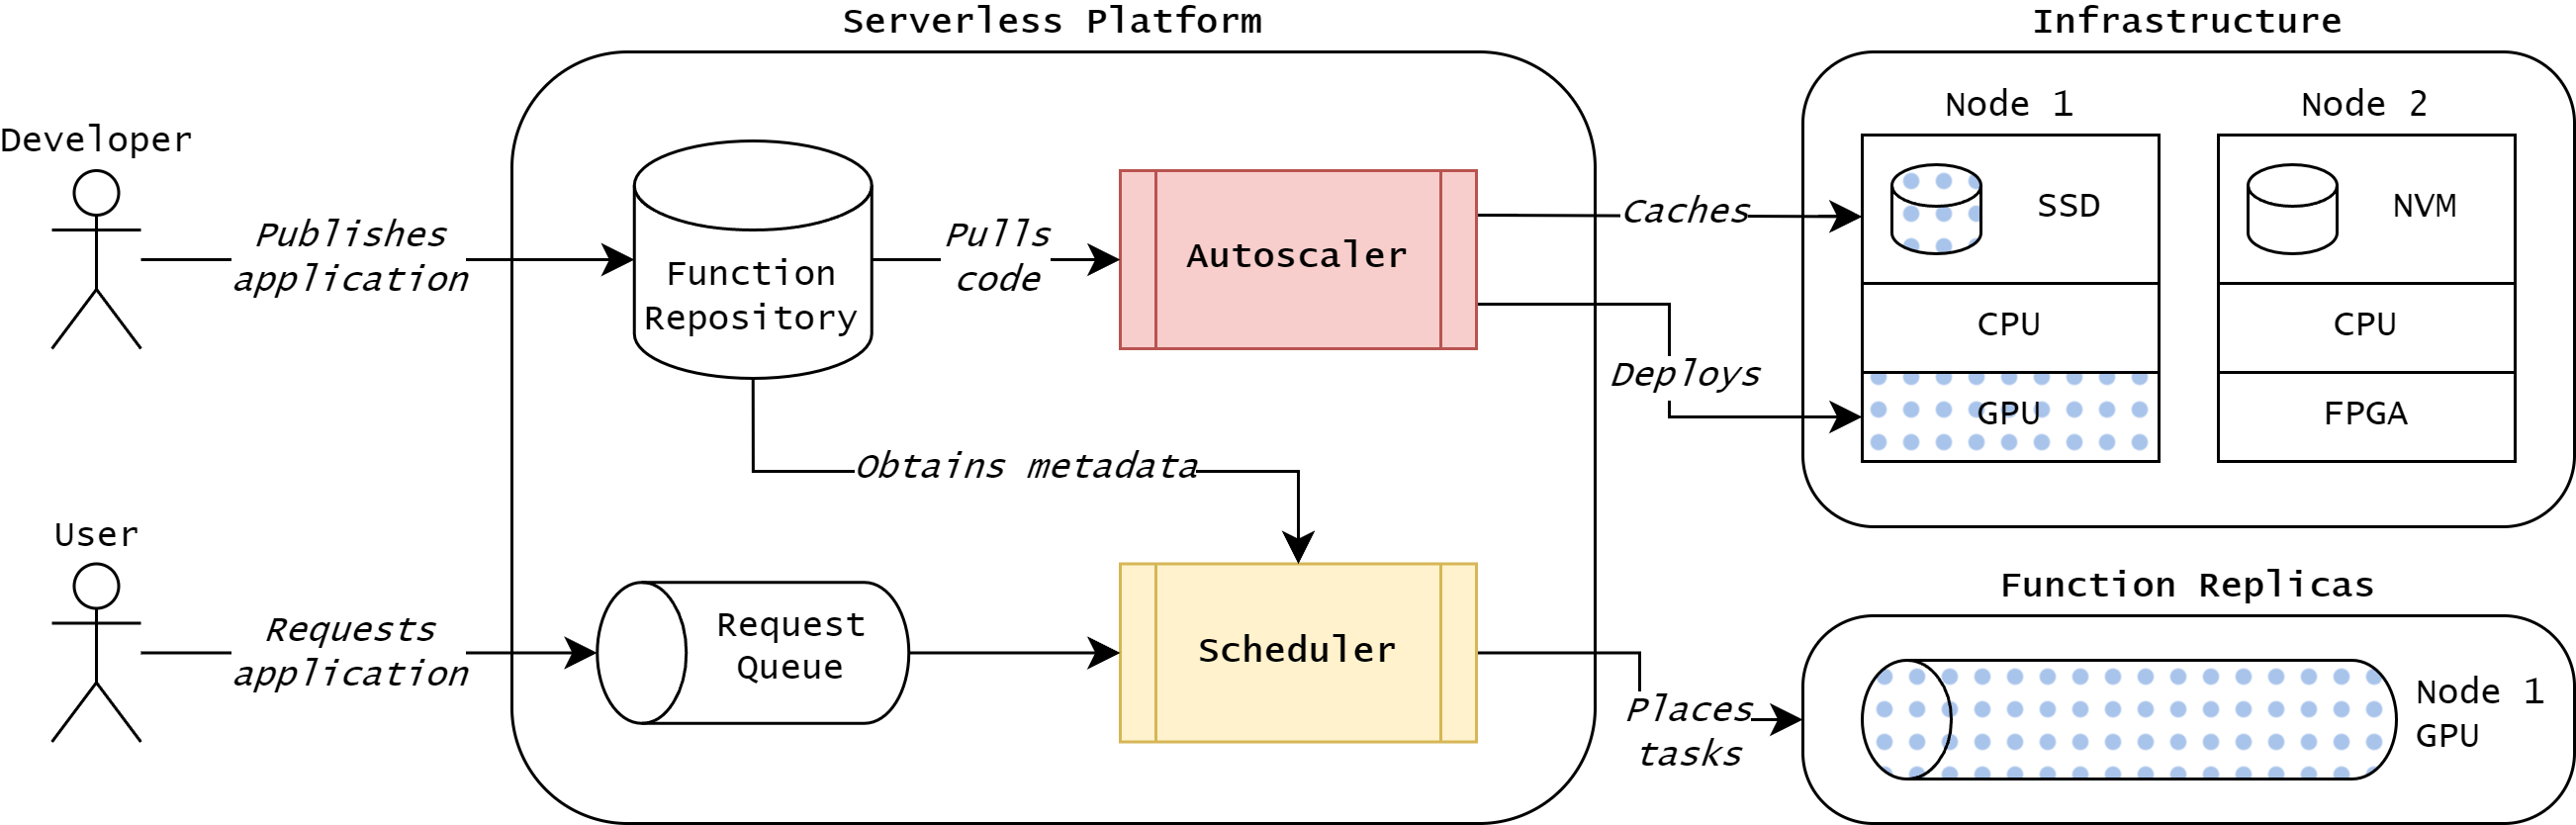
\includegraphics[width=0.9\textwidth]{7_Chapitre5/figures/platform.png}
    \caption{High-level view of a serverless platform, as modeled in HeROsim. The autoscaler allocates hardware resources for function replicas; while the scheduler places user requests in queue on those replicas.}
\label{figure:herosim-platform}
\end{figure*}

% Cloud infrastructure


%In cloud computing, customers typically book resources. These are usually a virtualized subset of heterogeneous hardware resources available on servers called nodes. Once the reservation has been made, service providers deliver remote access to the customer, who is responsible for the deployment of their applications and billed according to the amount of resources they reserved~\cite{Lannurien2023}.

% Functions, applications
In the serverless paradigm, customers start by pushing their code to a repository on the provider's side, see Figure~\ref{figure:herosim-platform}. %The provider allocates resources that are automatically scaled according to the load. 
For this mechanism to work, applications are divided into small steteless execution units called \textbf{functions}. %These functions are stateless~\cite{yuFollowingDataNot}. %: Should they produce any output data, these must be kept in persistent storage~\cite{yuFollowingDataNot}.

% Space-sharing, time-sharing -- different models
%In traditional service models, resources are scaled across two dimensions: horizontally (new application instances created on further nodes) and vertically (additional resources allocated to existing instances). 
In serverless platforms, resources are scaled horizontally: variations in load on applications are absorbed by adding new instances of the functions, called \textbf{replicas}, and removing them when no longer needed. A replica can be created for each user request or reused for multiple user requests. We can consider function replicas as request queues with different capacities.

% Autoscaler types (scale to zero, horizontal/vertical...)
These replicas are created by the \textbf{autoscaler}. To manage the number of replicas deployed for each function, there are three main strategies: request-based, concurrency-based, and metrics-based~\cite{mahmoudiSimFaaSPerformanceSimulator2021}. In request-based autoscaling, requests coming in the system are handled by idle replicas. If no idle replica is available, a new instance is created. In concurrency-based autoscaling, each replica can queue multiple user requests and handle them sequentially according to a predefined concurrency threshold~\cite{herofake}. In metrics-based autoscaling, the number of deployed replicas depends on various objectives, such as the request rate per second (RPS) to meet. %This requires monitoring the performance of the system for use by the autoscaler.

% Replica (function instance) state (initializing, running, idle)
Replicas can be in three different states: initializing, running, and idle.%~\cite{SchleierSmith2021WhatSC}. 
When a function replica has just been created, it is in initializing state: the platform instantiates its execution environment, pulls its code from a remote registry and optionally caches it on the deployment node, and starts executing the function. When the replica handles user requests, it is in running state. Otherwise, the replica is idle, and can be removed.
% Cold start problem, warm start, data-shipping architectures
When replicas are removed, hardware resources are freed. However, when a new replica is created to handle user requests, this incurs an overhead called a \textbf{cold start}. Orchestrators adopt various policies to mitigate this issue.% ranging from enforcing a keep-alive period on function replicas to avoid destroying them too early, to proactively allocating replicas.

% Scheduler policies (bin-packing, load balancing...)
Finally, user requests are mapped to the available function replicas by the \textbf{scheduler} that implements different strategies: for example AWS Lambda\footnote{\href{https://aws.amazon.com/en/lambda/}{https://aws.amazon.com/en/lambda/}} uses a bin-packing algorithm, while an open source platform such as Knative implements a load balancing policy~\cite{Lannurien2023}. %These strategies have different outcomes with regard to resource usage and QoS, but it can be difficult to predict to what extent they will impact workloads before deployment.

\section{Design of HeROsim}
\label{section:herosim-herosim}

%This section introduces the design choices and hypotheses made for the development of HeROsim.%, in order to help users get started implementing their own policy in simulation.

% \begin{figure}[t]
%     \centering
%     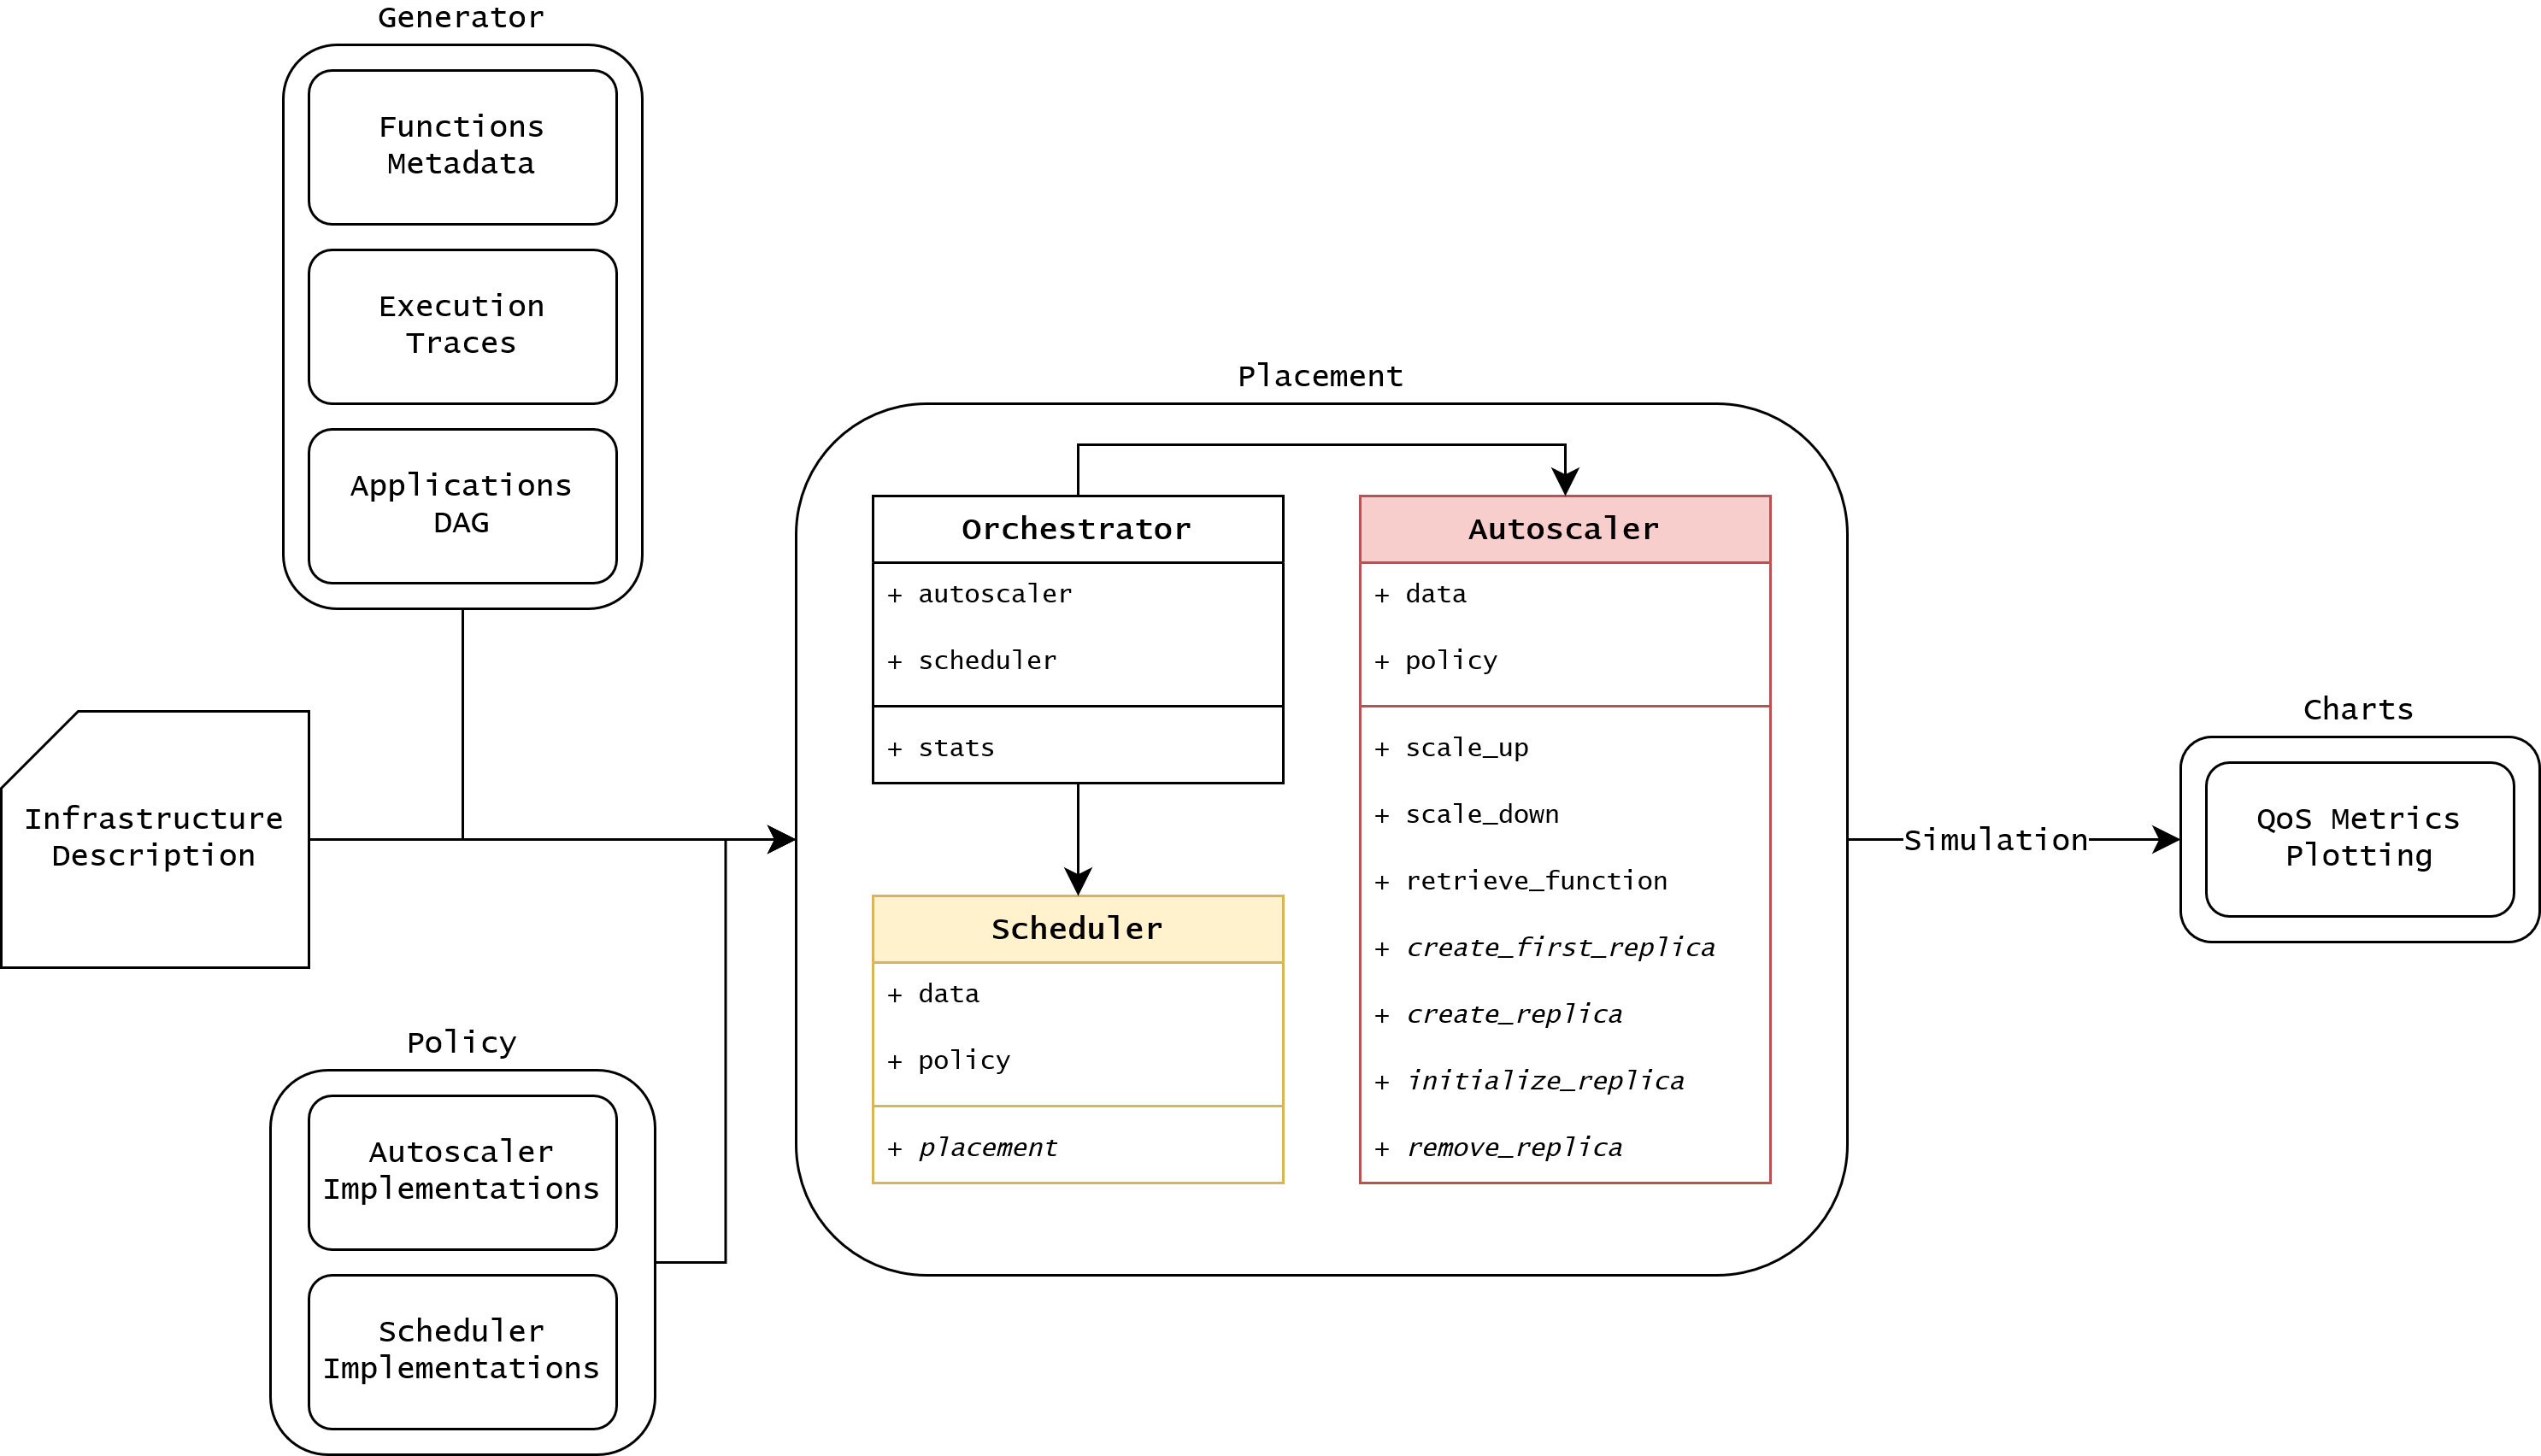
\includegraphics[width=\columnwidth]{7_Chapitre5/figures/software-architecture.png}
%     \caption{FIXME: High-level view of the simulator's architecture \jb{illisible}}
% \label{figure:herosim-software-architecture}
% \end{figure}

HeROsim uses the SimPy~\footnote{\href{https://simpy.readthedocs.io}{https://simpy.readthedocs.io}} library as the discrete-event simulation engine. It ships three base classes -- \texttt{Orchestrator}, \texttt{Autoscaler} and \texttt{Scheduler} -- that should be subclassed by users willing to implement their own  algorithms. As the bulk of the platform behavior is inherited from the base classes, implementation overhead for a new policy is minimal: the simplest couple of autoscaler and scheduler (Random Placement policy) are implemented in less than 20 LOCs.

\subsection{Input data}

HeROsim exposes a declarative interface for users to define their cloud environment, workloads and QoS constraints. The simulator replays an allocation and placement scenario under different orchestration policies. A simulator run requires the following JSON inputs to define such a scenario:

\begin{enumerate}
    \item A \textbf{workload description}; details on the \textbf{characteristics of the functions}  invoked during the scenario, \textit{i.e.} their execution time and cold start time, memory requirements, energy consumption, image size, input and output data size These metadata could be defined by \textbf{measuring} and \textbf{analyzing} the applications' behavior on a testbed configuration. % (see Figure~\ref{figure:herosim-characterization}).
    \item An \textbf{infrastructure description}; the listing of the different \textbf{nodes available}, their different hardware execution platforms, storage devices, network bandwidth. Execution platforms are defined in terms of idle energy consumption and retail price; storage devices are characterized by their capacity, bandwidth, and latency. These data are specific to a target platform and could be \textbf{measured} or obtained from manufacturers.
    \item An \textbf{execution trace}; the arrival times for all \textbf{user requests} to the applications, associated with their desired QoS level, in chronological order. These data can be extracted from real-world \textbf{observations} of the applications in production, or statistically estimated. % (see Figure~\ref{figure:herosim-characterization}), or statistically estimated. 
\end{enumerate}

Data from our previous studies~\cite{herofake, herocache} are available in the repository for reference. While (1) and (2) can be hand-written according to the use-case requirements, HeROsim provides a synthetic generator to create various traces for (3) using Poisson processes, with variable duration and user request rate, as commonly done in the literature~\cite{herocache}. 

\subsection{Simulation flow}

The user may choose the desired orchestration policies and execute the main program. The simulator will:

\begin{itemize}
    \item Initialize the infrastructure as described: the scenario starts with all the nodes idle, waiting for new requests.
    \item Initialize the orchestrator with chosen autoscaler and scheduler.
    \item Follow the arrival times of events from the execution trace, and pass the user requests to the orchestrator.
    \item Let the scheduler try to place these requests on function replicas.
    \item Let the autoscaler allocate and deallocate hardware resources that host these replicas to handle user requests.
\end{itemize}

% The simulation advances on \textbf{task executions}, \textit{i.e.} when functions are scheduled \jb{bizarre cette phrase}\vl{et comme ça ?}.

The simulation advances on handling user requests. The simulator knows the functions' response time based on the input metadata. % metadata measured beforehand. These metadata concern the specific hardware and workloads the user is interested in scheduling. They can be obtained in many ways; Figure~\ref{figure:herosim-characterization} shows an overview of the methodology we used to characterize various workloads and execution platforms throughout our experiments; see~\cite{herofake, herocache} for more details.

% \begin{figure}[t]
%     \centering
%     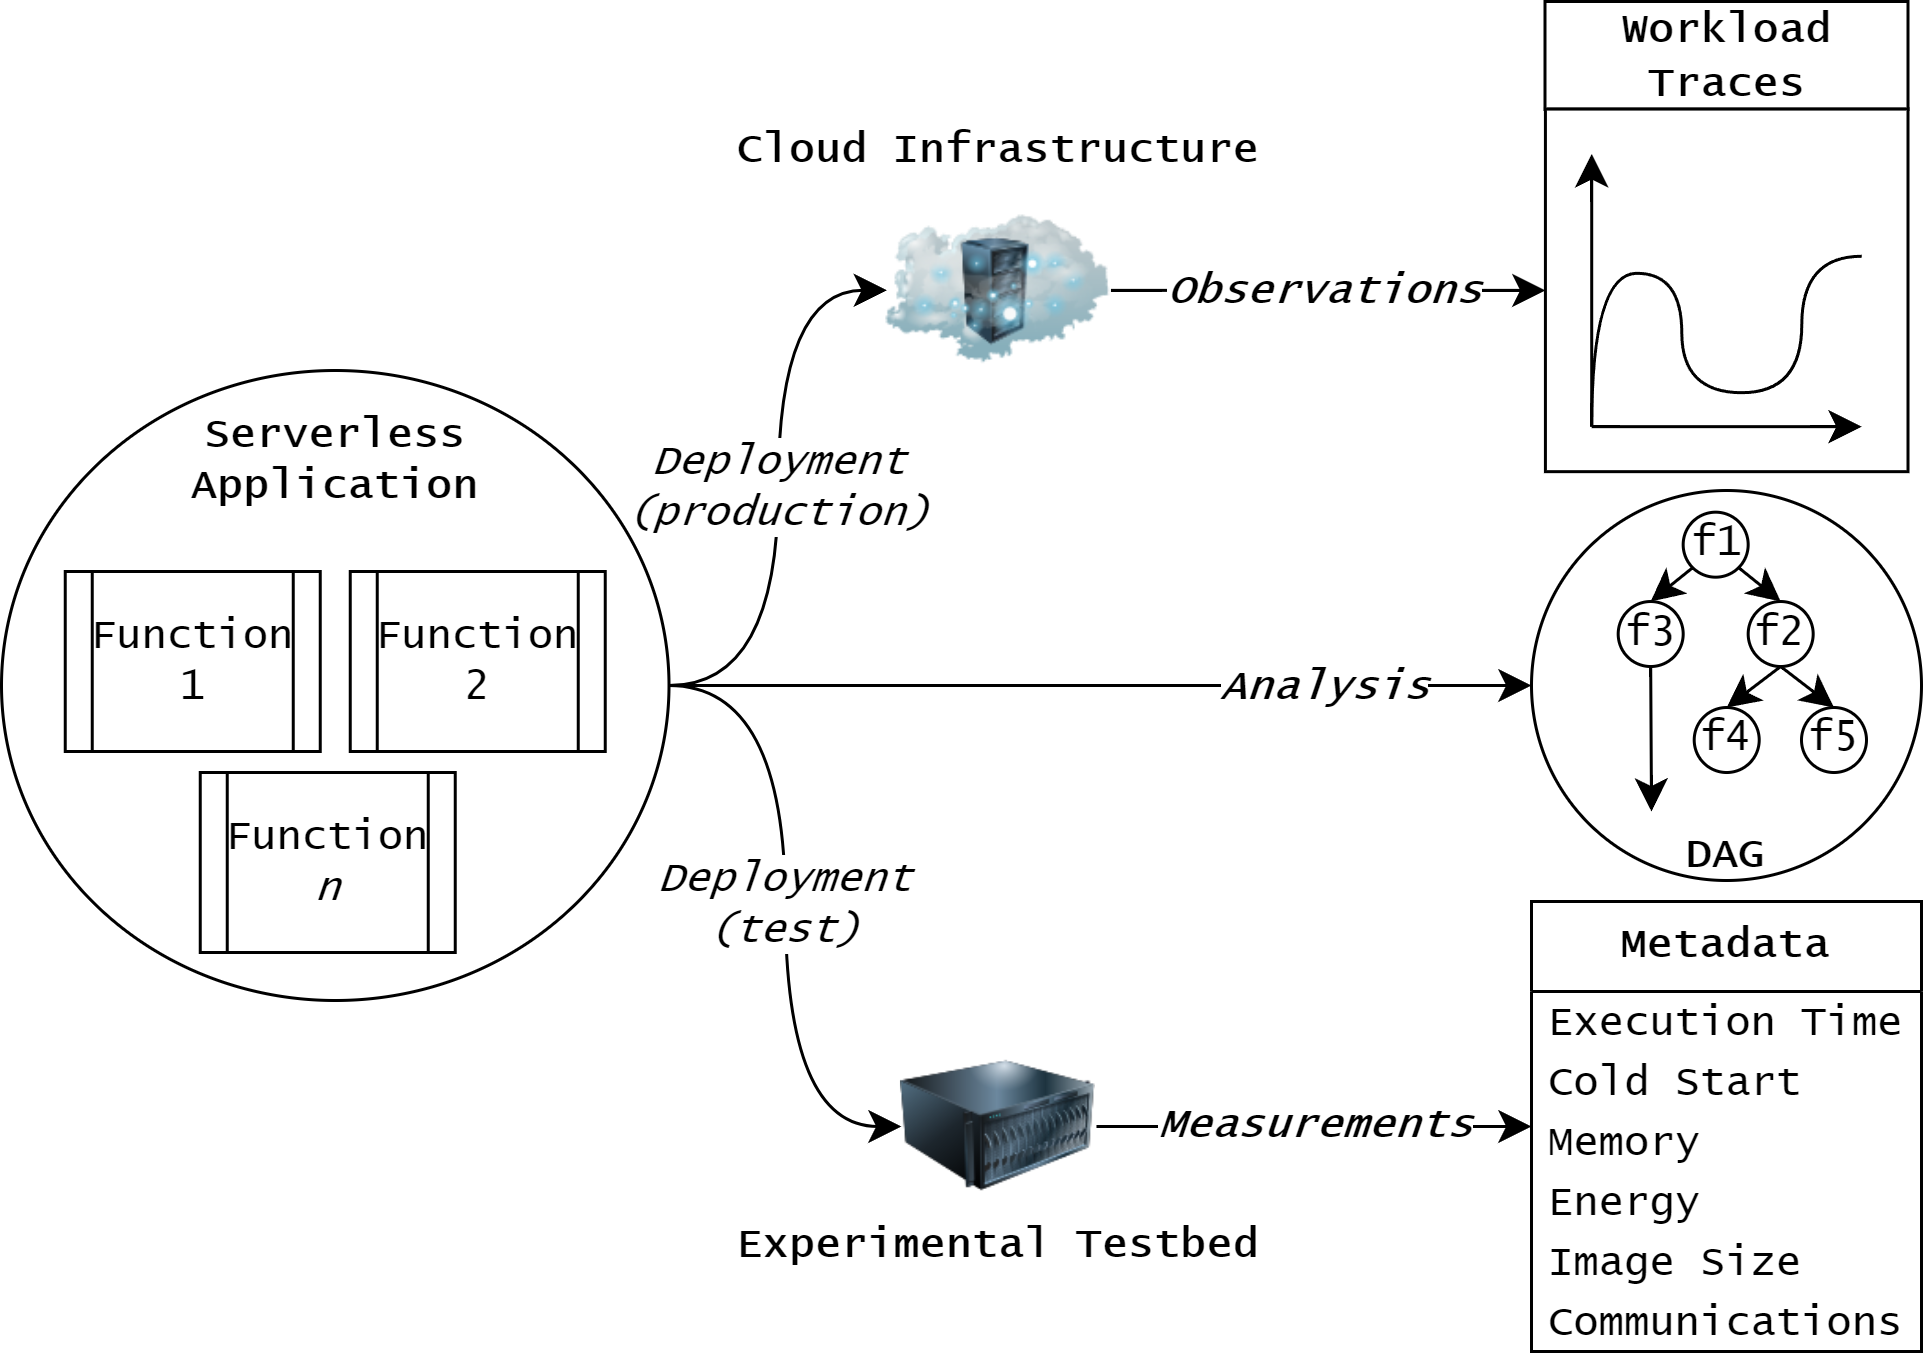
\includegraphics[width=\columnwidth]{7_Chapitre5/figures/characterization.png}
%     \caption{An overview of our characterization methodology.}
% \label{figure:herosim-characterization}
% \end{figure}

%During the simulation, logs are written to the disk. When all the user requests have been processed, the simulation stops and returns results and charts summarizing the simulation run. \vl{c'est expliqué dans User Interface, on peut le retirer ici} %, respectively in the \texttt{result} and \texttt{chart} directories.





%The simulator is single-threaded, meaning that each policy will be evaluated sequentially. However, multiple instances of HeROsim can be run in parallel with different configurations across multiple CPU cores, or distributed across multiple nodes. With every HeROsim instance running a different orchestration policy, and all instances using a common output directory, this can accelerate the total makespan of the simulation scenario when evaluating numerous orchestration policies. When all the simulator runs are finished, results can be consolidated in a single charts output. \jb{je pense que ce paragraphe peut sauter si manque de place, rien de très interessant}

\subsection{Orchestrator}

The base \textbf{\texttt{Orchestrator}} class provides abstract initialization methods that are to be overridden to manage different structures of system state. For example, a Round Robin scheduler would need to know how many times each function replica has been selected for task placement, while a Least Connected scheduler will need to know the average concurrency in each replica to balance the load. This class is the entry point for users to define their own data structures that will best represent the system state to feed the \texttt{Autoscaler} and \texttt{Scheduler} to manage.

Users can implement the system state management process they need to support their orchestration policies. The base orchestrator is provided with a simple system that can serve as-is, or be extended. %as an example for more advanced techniques. 
In our implementation, a monitoring process is called periodically to keep track of the average concurrency in each function replica. This is useful for threshold-based policies.

The orchestrator entrypoint method is called each time a user request hits the platform. It takes the system state and the user request as input. It can be overridden in each orchestration policy implementation to enable fine-grained autoscaling and scheduling as needed.

Finally, this class is responsible for instantiating the selected implementations of \texttt{Autoscaler} and \texttt{Scheduler}. Any combination of these two modules can work together.

%\jb{pour chaque module plus bas, il manque une information claire indiquant quelles stratégies sont impléménentées par ce module. Peut être rajouter une phrase à la fin de chaque module pour dire voila les stratégies implémentées.}\vl{done}
\subsection{Autoscaler}

The base \textbf{\texttt{Autoscaler}} class provides the common behavior of the autoscaling platform, including the creation and removal of function replicas. Several abstract methods have to be overridden to implement a new policy: resource selection for replica creation, replica initialization process, replica selection for removal, etc. These methods operate at the granularity of a single function, taking the system state and the list of available hardware resources as input. %Users are free to implement whichever algorithms they wish to evaluate for resource management.

HeROsim's autoscaler was primarily designed for horizontal scaling. Function replicas are created by allocating one execution platform and the required amount of peak memory on a node. An execution platform cannot host more than one function replica at a time. To accommodate higher load on an application without QoS degradation, new function replicas need to be allocated by the autoscaler, provided that enough hardware resources are available. Newly allocated replicas will go through an initialization phase during which function images have to be retrieved through the network. The autoscaler can manage an image cache in node memory and on node-local storage to accelerate cold starts.

Removing idle replicas is done on a best-effort basis: the autoscaler tries to remove replicas with empty task queues. By default, a replica with pending tasks cannot be removed.

The autoscaler keeps track of each allocation event to compute resource usage at the end of the simulation. HeROsim allows the user to know which nodes and execution platforms have been enrolled during the scenario, at which time and for which duration, and for which function deployment they were chosen. This also enables HeROsim to compute energy consumption at different granularities: static power needed by allocated hardware, and dynamic power used by applications during their execution.

HeROsim ships with the following concurrency threshold-based ready-to-use autoscaling policies:

\begin{itemize}
    \item Random -- Selects a random node and execution platform for new replicas.
    \item Knative -- Selects the least loaded node to allocate new replicas, \textit{i.e.} balances workloads across a large number of nodes.
    \item HeROfake -- Leverages hardware heterogeneity to minimize QoS penalties, energy consumption and Total Cost of Ownership. %More details are given in the "Case study" section.
    \item HeROcache -- Optimizes allocations for functions chains; maximizes consolidation functions of each application. %More details are given in the "Case study" section.
\end{itemize}

\subsection{Scheduler}

The base \textbf{\texttt{Scheduler}} class implements task selection in the gateway queue. One abstract method has to be overridden to implement a new policy: the selection of replica among the pool to place each user request in queue. This method operates at the granularity of one user request and takes the system state and the list of available function replicas as input.

User requests arrive in a queue at the scheduler level. Users can implement their own priority policy for task selection, or choose a policy already available in the simulator, \textit{e.g.} FIFO or Earliest Deadline First~\cite{herofake}.

HeROsim's scheduler has been designed without task failure or migrations in mind: the default behavior considers tasks that always run to completion on their replica. However, tasks will be marked as "in penalty" if scheduling misses their deadline. Users can leverage this boolean value to evaluate the quality of their policies with regard to request latency: it indicates what proportion of requests are handled in a timely fashion. 

%If there is no replica available at the time of scheduling a user request, the scheduler will make a call to the autoscaler to force the creation of a first replica for the function. In the meantime, the request will be put back in queue and postponed. Postponed tasks are flagged as such, so that, for instance, they can have higher priority if the user wants to enforce such a policy~\cite{herocache}. \vl{paragraphe pas forcément indispensable ? c'est un "cas particulier" (scale from zero) de l'autoscaler}

HeROsim ships with the following scheduling policies implemented and ready to use:

\begin{itemize}
    \item Random -- Selects a random replica for task placement.
    \item Knative -- Selects the replica with the shortest in-flight request queue for task placement.
    \item BPFF -- Selects the replica with the longest in-flight request queue for task placement.
    \item HeROfake -- Selects the replica that minimizes a compound score according to the task's deadline, energy consumption of the function and scattering of tasks across nodes. %More details are given in the "Case study" section.
    \item HeROcache -- Selects the replica similar to HeROfake, but takes the storage and commuincation into account. %operations into account to compute the request's end-to-end latency, and takes the functions chains into account when scoring replicas with regards to tasks consolidation. %More details are given in the "Case study" section.
\end{itemize}


\subsection{User interface}

%Interactions between the user and the simulator are limited. 
HeROsim relies on logging to provide insight as to how the simulation unwinds, helping the user debug their policies. When the simulation ends, result files are saved to disk. These files contain digest information on the results of the simulation, including the performance of the policy with regards to evaluation metrics. These results are plotted on various charts that can be used in further publications (see Figure~\ref{figure:herosim-evaluation}). HeROsim can also plot cold starts, cache hits and tail latency at the granularity of user requests. %\vl{viré le paragraphe dessous et résumé en 1 phrase}

% HeROsim can also generate additional charts that can be of use when debugging the behavior of an orchestration policy. Users can visualize the proportion of cold starts and cache hits across function invocations. HeROsim can plot tail latency for all user requests, helping the user rightsize their infrastructure. The execution trace generator will plot requests inter-arrival times on a chart to provide visual cues on the characteristics of the workload.

%There is ongoing work on extending HeROsim to propose a web interface to visualize the simulation state in real time. This interface might be shipped with a future version of the simulator.

\begin{figure}[t]
    \centering
    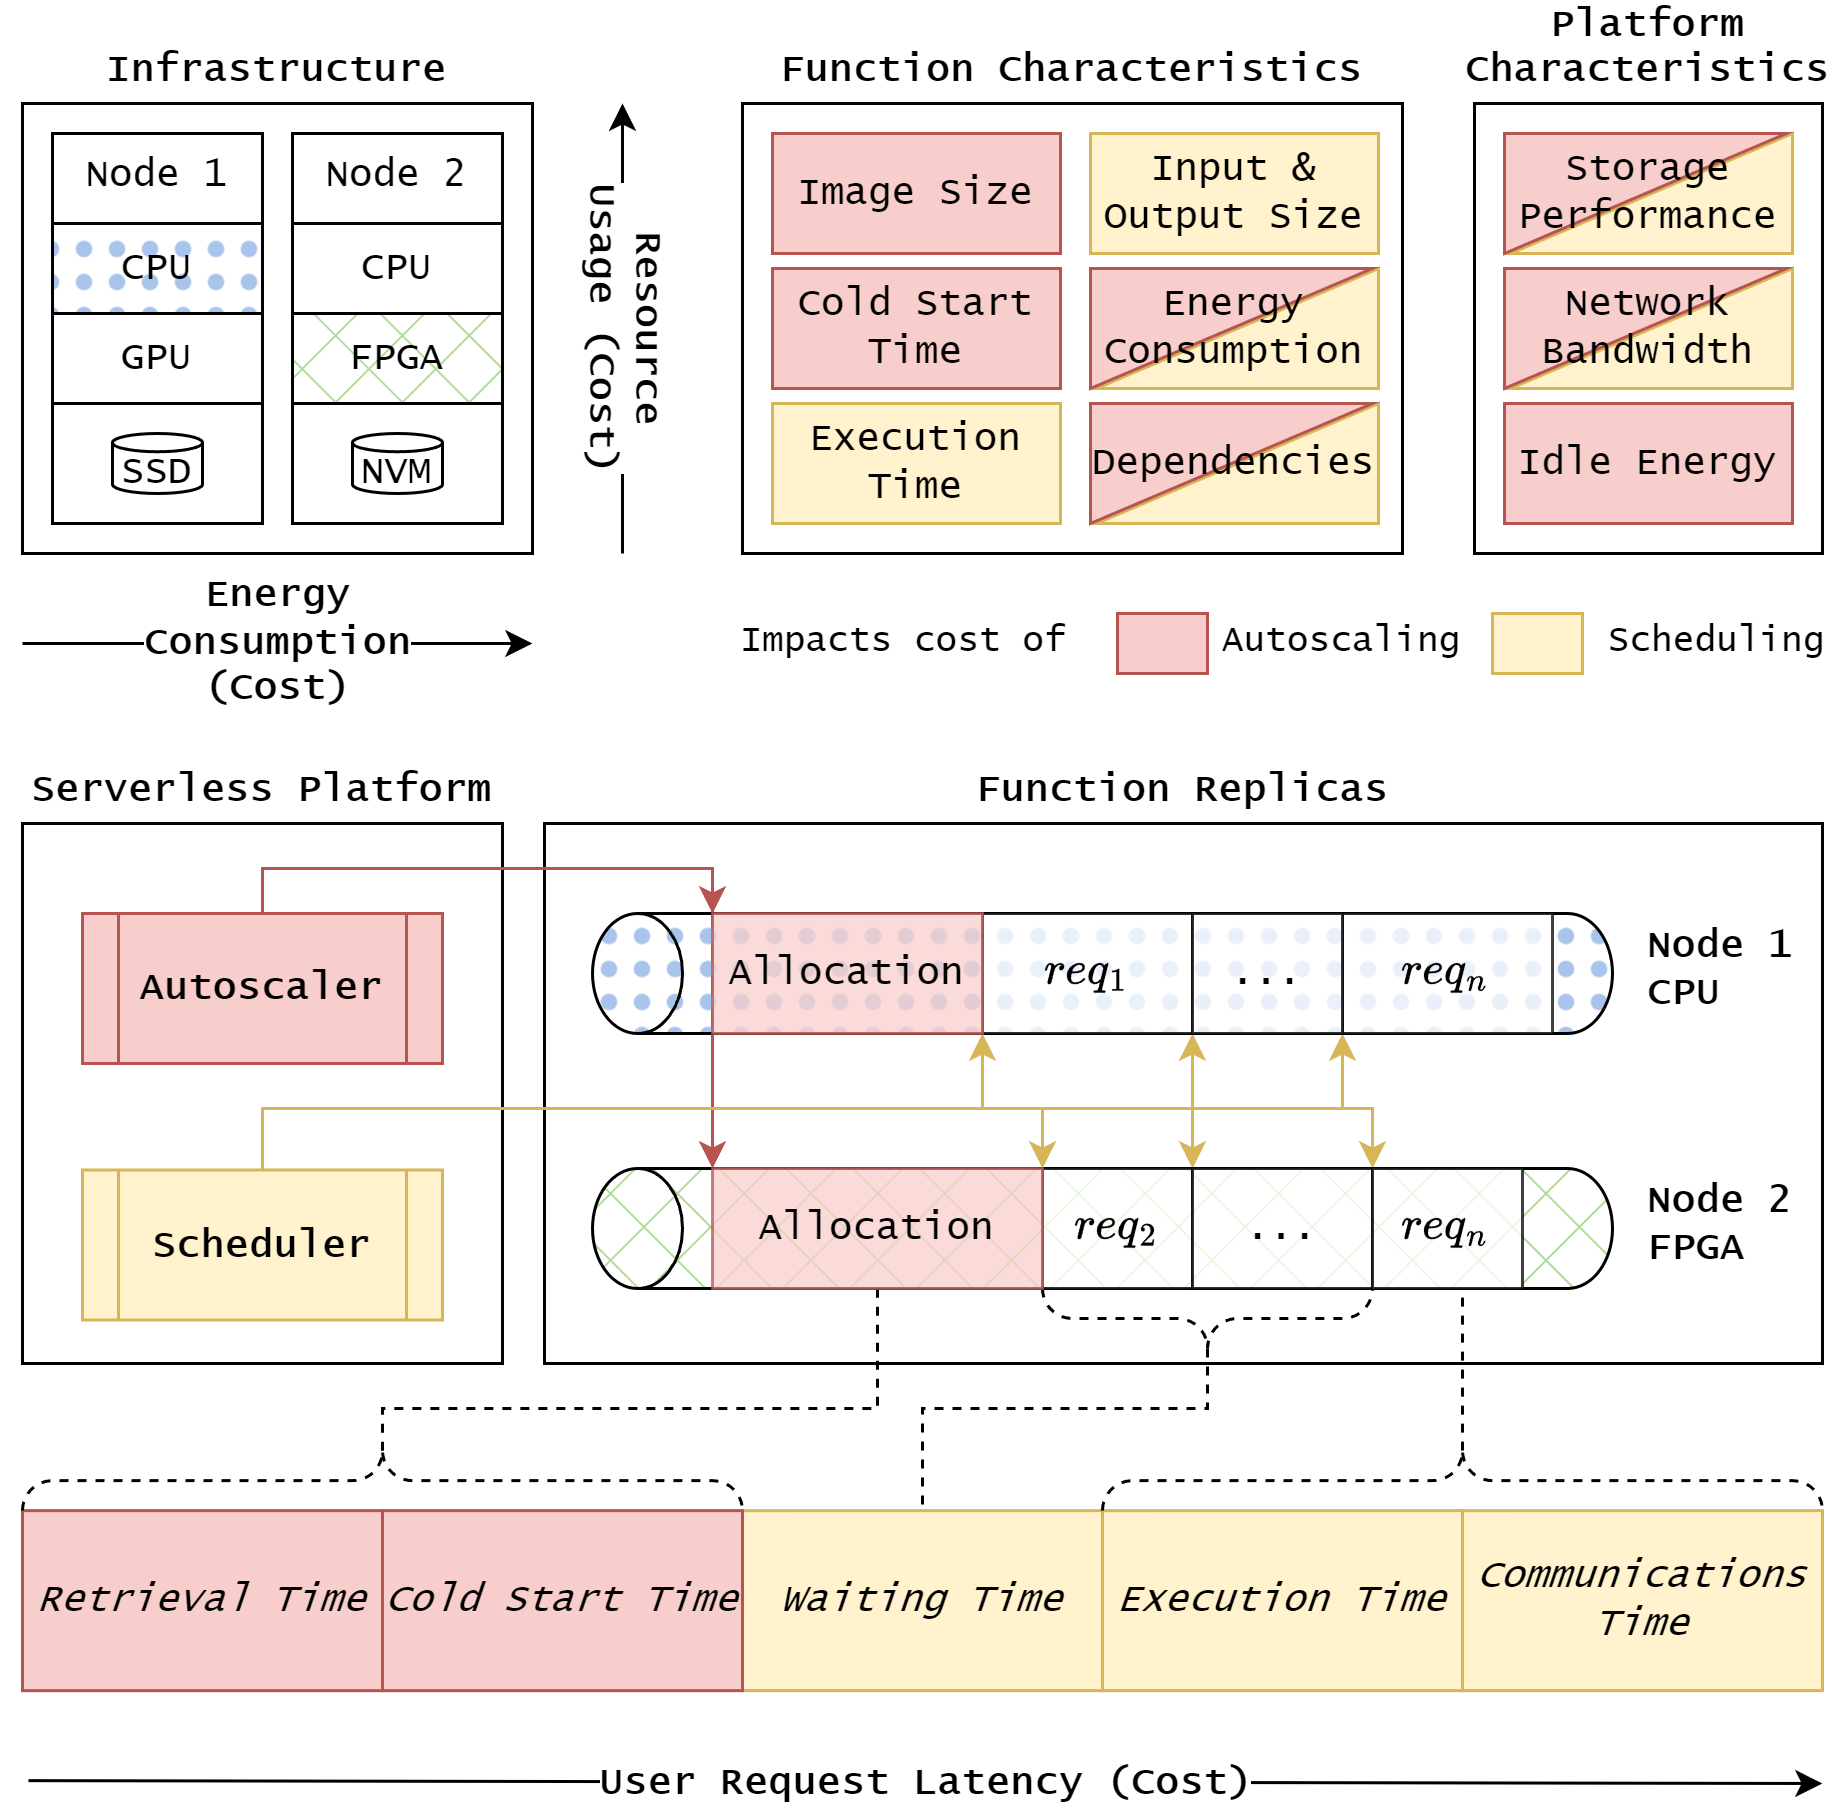
\includegraphics[width=\columnwidth]{7_Chapitre5/figures/serverless-cost.png}
    \caption{Breakdown of the end-to-end latency cost incurred by autoscaling and scheduling decisions.}
\label{figure:herosim-cost}
\end{figure}

\section{Case study}
\label{section:herosim-case-study}

%\jb{je ne m'attendais pas à cela dans la section case study. Je m'attendais plutôt à une section plus conséquente ou l'on donne clairement comment passer du pb à la mise en oeuvre sur le simulateur avec un peu plus de détails techniques. la, ça fait un peu commercial, on donne juste les résultats}\vl{section complètement réécrite}

\begin{figure*}[t]
    \center
    \subfloat[Consolidation\label{figure:herosim-evaluation-full-unused-nodes}]{
        \includegraphics[width=0.155\linewidth]{7_Chapitre5/figures/eval/2-unused-nodes.png}
    }
    \subfloat[QoS\label{figure:herosim-evaluation-full-penalty}]{
        \includegraphics[width=0.155\linewidth]{7_Chapitre5/figures/eval/3-penalty-proportions.png}
    }
    \subfloat[Energy\label{figure:herosim-evaluation-full-energy-consumption}]{
        \includegraphics[width=0.155\linewidth]{7_Chapitre5/figures/eval/6-energy-consumption.png}
    }
    \subfloat[Consolidation\label{figure:herosim-evaluation-components-unused-nodes}]{
        \includegraphics[width=0.155\linewidth]{7_Chapitre5/figures/eval-components/2-unused-nodes.png}
    }
    \subfloat[QoS\label{figure:herosim-evaluation-components-penalty}]{
        \includegraphics[width=0.155\linewidth]{7_Chapitre5/figures/eval-components/3-penalty-proportions.png}
    }
    \subfloat[Energy\label{figure:herosim-evaluation-components-energy-consumption}]{
        \includegraphics[width=0.155\linewidth]{7_Chapitre5/figures/eval-components/6-energy-consumption.png}
    }
    \caption{Charts generated by HeROsim for the evaluation of HeROcache -- Comparison against baselines (a-c) and impact of individual components (d-f). HRC-HRO means HeROcache autoscaler coupled with HeROfake scheduler.}
    \label{figure:herosim-evaluation}
\end{figure*}

%This simulation tool has been developed to support research work on orchestration policies in private serverless cloud. We argued that various challenges limit the relevance of serverless for users, and hinders the cost efficiency of the model for service providers:

% \begin{itemize}
%     \item The absence of QoS guarantees in serverless platforms prevents meeting the users' requirements in different use cases~\cite{Lannurien2023}.
%     \item Serverless platforms consider the underlying infrastructure as homogeneous and miss on the opportunity to further optimize task placements~\cite{herofake}.
%     \item Most orchestrators do not consider the costs linked with storage operations that can dominate functions' execution time~\cite{herocache}.
% \end{itemize}

%We investigated the design of a serverless platform that would tackle these challenges. Implementing the software necessary for our experiments would have been time-consuming, hence resorting to simulation was considered a more cost-efficient approach.

We present two case studies that made use of HeROsim to evaluate orchestration policies.
We devised strategies that rely on heterogeneous platform and workload characterization. % (see Figure~\ref{figure:herosim-characterization}).
%We measured several metrics related to our applications on various hardware platforms. 
We proposed a cost model that integrates these values to estimate the performance of autoscaling and scheduling under different policies, see Figure~\ref{figure:herosim-cost}.

% In both studies, we used HeROsim to evaluate our policies against various baselines, as well as to individually measure the impact of different autoscaler and scheduler configurations. Figure~\ref{figure:herosim-evaluation} shows the output charts that the simulator generated while evaluating HeROcache.



%\jb{dans ton intro, tu as indiqué des critères qu'un simulateur doit avoir. il faudrait dans la partie case study, dire dans des section séparaées comment chaque critère est pris en compte par case study. Je pense que ça serait interessant.}\vl{done}

\subsection{HeROfake}
% TODO: On-demand deepfake detection (inference tasks)
% TODO: Stateless tasks, no dependencies

In this first case study, \textbf{He}terogeneous \textbf{R}esources \textbf{O}rchestration for deep\textbf{fake} detection~\cite{herofake}, we investigated the deployment of a deepfake detection application on a serverless platform in a private cloud. %In particular, we were interested in leveraging heterogeneous resources for serverless orchestration when optimizing the platform for QoS and energy consumption.

The application runs inference tasks to detect deepfakes in potentially tampered-with images, submitted by users with various QoS level requirements. % Its objective is to detect potentially tampered-with images; pictures that might have been computer-manipulated to mislead viewers.
It consists of three independent and stateless neural network tasks that were implemented on heterogeneous hardware: CPU, GPU and FPGA. %These implementations were used for measurements.%, but it would have been challenging to actually run real-world scenarios on a serverless platform including these hardware architectures.

% TODO: Challenges: per-request QoS requirements, leverage heterogeneous hardware, scarcely available, actual executions impossible

%HeROfake did not consider applications (functions chains), hence user requests corresponded to single task executions. 
In HeROfake, each task execution has an associated cost measured in \textbf{latency}. Allocating new replicas on idle hardware resources introduces a \textbf{cold start delay}; handling user requests on different hardware has various \textbf{function execution time}. Latency for each user request is ultimately compared with the request's \textbf{QoS requirement}: if the request deadline was missed, the task is in \textbf{penalty}. These elements constitute the basis of our cost model, see Figure~\ref{figure:herosim-cost}.

% TODO: Strategy: cost minimization, heterogeneous threshold-based autoscaling, EDF scheduling

Different hardware architectures also have different monetary and energy costs that were factored in the cost model. We implemented an autoscaler and a scheduler policy that seek to estimate and minimize this composite cost at the granularity of each user request. The autoscaler seeks to allocate platforms that minimize the overall cost, including resource usage, energy consumption and Total Cost of Ownership. The scheduler seeks to select replicas that handle requests with least penalties and lowest energy consumption.

% TODO: Scenario

% TODO: HeROfake was evaluated using a synthetic scenario with uniform distribution of request inter-arrival times, function calls and QoS levels.

% TODO: Results

%HeROfake proved to perform well (in terms of QoS penalties, consolidation, and energy) against Knative (Google's serverless orchestrator) and Bin-Packing First Fit (Amazon's policy in Lambda)~\cite{herofake}. 

%Our main goal was to investigate the relevance of taking hardware heterogeneity into account when allocating resources and scheduling user requests with regards to various QoS metrics, \textit{i.e.} end-to-end latency and energy consumption.

%Experimental results showed that while total task execution time in HeROfake is similar to vanilla Knative, we achieve more than 60\% reduction in QoS penalties; tasks are consolidated on less than 40\% of the infrastructure's nodes, with 77\% execution platforms left unused; and dynamic energy consumption is reduced by 35\% as compared to Knative.

%HeROsim also allowed us to evaluate the impact of the individual components of our framework. Results showed that, even allocating CPUs only, scheduling inference tasks with our QoS-aware policy could keep SLA violations under 50\%. 


\subsection{HeROcache}

% TODO: Intermittent intrusion detection (pre-processing and inference tasks)

Here, a \textbf{He}terogeneous \textbf{R}esources \textbf{O}rchestration with a \textbf{cache} strategy for a storage-aware execution was deisgned. We explored the deployment of an Intrusion Detection System (IDS) on a serverless platform. In particular, we explored the benefits of data-aware orchestration when leveraging heterogeneous hardware to deploy time-sensitive applications on resources-constrained edge devices.%, from the perspective of the service provider.


%The goal of the application is to detect potentially malicious TCP traffic in user-submitted networking logs. As this IDS application is specifically targeted at drones missions, its access pattern is tightly related to seasonal patterns that make it a good fit for the serverless paradigm.

% TODO: Stateful application, temporal and data dependencies

The application consists of two layers: two preprocessing functions that operate on logs of network traffic, and four inference functions that detect patterns of malicious activity in the logs. These functions have been implemented on various edge hardware architectures (CPUs, FPGA, GPU). 

% TODO: Challenges: dependencies between functions, resources-constrained edge nodes, slow communications through remote storage, node-local storage contention (function cache vs intermediate data storage)
There are data dependencies between the two layers of the application. We modeled them as a Directed Acyclic Graphs (DAG) of function calls. % We used Python's \texttt{TopologicalSorter} from the \texttt{graphlib} module for JSON representation of the graphs and to traverse them during runtime.

%At the orchestrator level, we had to change the granularity of user requests: a user request concerns an application, which can be made up of one or more functions, called in the order defined by the application's DAG. Each function can take input data and produce output data. These data are defined by their size in bytes.

% TODO: Strategy: consolidation of applications' functions to minimize remote storage use, dependencies pre-fetching in cache for cold start acceleration

While HeROfake did not consider storage operations, HeROcache implements \textbf{function image retrieval}, \textbf{function image caching} and \textbf{inter-function communications} in the base orchestrator. These operations add up to user request latency by an amount of time computed on the basis of platform and function characterization, see Figure~\ref{figure:herosim-cost}. %: for example, HeROsim estimates function image retrieval time based on the network bandwidth specified by the user in the infrastructure description, the function image size specified by the workload type, and the node-local storage performance specified by the storage type.

%Introducing storage operations at individual node level allowed us to evaluate a function image prefetching strategy to accelerate cold starts in future invocations.

In HeROcache, the autoscaler seeks increased function consolidation across applications, reduced overall makespan, energy consumption and Total Cost of Ownership. The scheduler seeks to avoid missed request deadlines, use less power and enforce high resource usage.

% TODO: Workload characterization, synthetic workload trace based on a Poisson process, 4G LTE request rate

% We used the execution trace generator included in HeROsim to generate a 30-minute scenario of user requests following a Poisson process at an average rate of 83 Requests per Second. This corresponds to the rate of communications that 4G LTE connectivity would allow in our edge setting, given the size of the application input and output data. 

% TODO: Results

Evaluation against HeROfake highlighted the relevance of taking into account storage operations, see Figure~\ref{figure:herosim-evaluation}.

% We evaluated HeROcache against various baselines (Knative, BPFF, RP) and also against HeROfake, see Figure~\ref{figure:herosim-evaluation}.

%As HeROfake already leveraged hardware heterogeneity but was designed as a storage-oblivious policy, it made for a comparable solution. 
%This comparison allowed us to show the relevance of storage costs in QoS compliance  %showed that, with a data-aware orchestration policy, HeROcache enforces applications consolidation and manages to reduce average initialization delays by 17.6\% and communication delays by 88.4\%. This results in reducing the static energy consumption of the platform by 80\% while maintaining under 28\% of QoS violations.\jb{on peut raccourcir je pense}

%HeROcache (implemented on top of HeROsim) has been submitted for artifacts evaluation and received the three IEEE reproducibility badges~\footnote{\href{https://www.niso.org/standards-committees/reproducibility-badging}{https://www.niso.org/standards-committees/reproducibility-badging}}: Open Research Objects (ORO), Reusable/Research Objects Reviewed (ROR), and Results Reproduced (ROR-R).


% To address these issues, we proposed:
% \begin{itemize}
%     \item HeROfake~\cite{herofake}, a framework for the deployment of short-lived, interactive deepfake detection tasks on a private, heterogeneous serverless cloud. Experimental results showed that while total task execution time in HeROfake is similar to vanilla Knative, we achieve more than 60\% reduction in QoS penalties; tasks are consolidated on less than 40\% of the infrastructure's nodes, with 77\% execution platforms left unused; and dynamic energy consumption is reduced by 35\% as compared to Knative.
%     \item HeROcache~\cite{herocache}, an allocation and scheduling policy for serverless edge computing that seeks to optimize time-sensitive applications deployment for QoS on energy-constrained devices. HeROcache enforces applications consolidation and manages to reduce average initialization delays by 17.6\% and communication delays by 88.4\%. This results in reducing the static energy consumption of the platform by 80\% while maintaining under 28\% of QoS violations.
% \end{itemize}

\section{Related work}
\label{section:herosim-sota}
%\jb{c'est TROOOP long !!!, ce n'est pas les related work qui feront que le papier sera accepté, une colonne c'set amplement suffisant. Il faut renforcer la contrib et le case study absolument !!} \vl{ok, on raccourcira à la fin, ce sera facile. j'ai détaillé chaque contrib et je les ai aussi regroupées par caractéristique. On peut garder uniquement les regroupements et virer les détails individuels.}\jb{ok} \vl{done, j'ai gardé les grandes familles (CloudSim, GridSim), j'ai fait les regroupements qui me semblaient pertinents et j'ai raccourci la section à environ une colonne}

\begin{table*}[t]
    \centering
    \caption{Overview of simulation tools for cloud computing}
    \resizebox{\linewidth}{!}{
        \begin{tabular}{lSSSSSSSSS}
        \toprule
        & Serverless & Deployment models & Functions chains & Hardware heterogeneity & Per-request QoS & Resource usage & Energy consumption & Visualization \\
        \cmidrule(lr){2-2}\cmidrule(lr){3-3}\cmidrule(lr){4-4}\cmidrule(lr){5-5}\cmidrule(lr){6-6}\cmidrule(lr){7-7}\cmidrule(lr){8-8}\cmidrule(lr){9-9}
        CloudSim~\cite{calheiros_cloudsim_2011} & \xmark & Public, private, hybrid & \xmark & \cmark & \xmark & \cmark & \cmark & \xmark \\
        CloudSimSC~\cite{mampage_cloudsimsc_2023} & \cmark & Public, private, hybrid & \xmark & \cmark & \xmark & \cmark & \cmark & \xmark \\
        CloudAnalyst~\cite{wickremasinghe_cloudanalyst_2010} & \xmark & Public, private, hybrid & \xmark & \cmark & \xmark & \cmark & \cmark & \cmark \\        DFaaSCloud~\cite{jeonCloudSimExtensionSimulatingDistributed2019} & \cmark & Multi-tier hybrid cloud & \xmark & \xmark & \cmark & \cmark & \xmark & \cmark \\
        ElasticSim~\cite{cai_elasticsim_2017} & \xmark & Public & \cmark & \xmark & \xmark & \cmark & \xmark & \cmark \\
        GridSim~\cite{buyyaGridSimToolkitModeling2002} & \xmark & Grid & \xmark & \cmark & \cmark & \cmark & \xmark & \cmark \\
        iCanCloud~\cite{nunez_icancloud_2012} & \xmark & Public & \xmark & \xmark & \xmark & \cmark & \xmark & \cmark \\
        iFogSim2~\cite{mahmudIFogSim2ExtendedIFogSim2021} & \xmark & Edge, Fog & \xmark & \cmark & \xmark & \cmark & \cmark & \xmark \\
        OpenDC 2.0~\cite{mastenbroekOpenDCConvenientModeling2021} & \cmark & Public, private, hybrid & \cmark & \cmark & \xmark & \cmark & \cmark & \cmark \\
        SimFaaS~\cite{mahmoudiSimFaaSPerformanceSimulator2021} & \cmark & Public & \xmark & \xmark & \xmark & \cmark & \cmark & \cmark \\
        \textbf{HeROsim} & \cmark & Private & \cmark & \cmark & \cmark & \cmark & \cmark & \cmark \\
        \bottomrule
        \end{tabular}
    }
    \label{table:herosim-sota}
\end{table*}

We present an overview of state-of-the-art work and their characteristics in Table~\ref{table:herosim-sota}.

CloudSim~\cite{calheiros_cloudsim_2011} is the ubiquitous tool for large-scale cloud deployment experiments. It targets the different service models in traditional cloud computing. 
CloudSim, and its extensions~\cite{calheiros_cloudsim_2011, mampage_cloudsimsc_2023, wickremasinghe_cloudanalyst_2010, jeonCloudSimExtensionSimulatingDistributed2019} do not consider serverless applications, \textit{i.e.} the composition of functions to achieve complex behavior which introduces specific challenges.% (cold start delays, overhead from inter-function communications, etc.~\cite{wawrzoniakBoxerDataAnalytics2021a}). 
To address these particular problems, it is necessary to introduce storage management, as well as the handling of function chains as HeROsim does. % allows users to model such applications, and devise orchestration policies that are application-aware and can provide QoS benefits.

% DFaaSCloud~\cite{jeonCloudSimExtensionSimulatingDistributed2019} is another CloudSim-based simulator for distributed serverless computing. This work focuses on the geographical distribution of function instances across a cloud, edge and fog infrastructure. It helps estimating delays induced by function locality. Users define their functions in terms of latency constraints and DFaaSCloud provides a placement policy that minimizes violations and cost. As such, the premise of DFaaSCloud is specific to addressing the problem of geographical placement of tasks in a multi-tier Function as a Service environment, and does not pertain to the general challenges in serverless computing.

% ElasticSim~\cite{cai_elasticsim_2017} also extends CloudSim to provide dynamic resources allocation for cloud workflows, \textit{i.e.} chains of connected tasks not dissimilar to serverless applications. However, it does not consider the underlying heterogeneity in hardware resources, nor does it allow to enforce per-request QoS objectives. OpenDC 2.0~\cite{mastenbroekOpenDCConvenientModeling2021} also allows the user to model such function chains, and while this tool does allow modeling a heterogeneous datacenter and estimate its energy consumption, it also does not consider the variety of user requirements in terms of latency.

GridSim~\cite{buyyaGridSimToolkitModeling2002} has interesting characteristics, from modeling highly heterogeneous infrastructures to enforcing per-request QoS constraints. However, its focus on grid computing makes it unsuitable to explore dynamic resource allocation problems. iFogSim2~\cite{mahmudIFogSim2ExtendedIFogSim2021} also considers static allocations that cannot faithfully characterize the serverless problem space. HeROsim has been designed for the serverless problem space and allows users to trace dynamic allocation and scheduling events at a user request granularity.

Multiple contributions~\cite{jeonCloudSimExtensionSimulatingDistributed2019, cai_elasticsim_2017, buyyaGridSimToolkitModeling2002, nunez_icancloud_2012} do not allow one to estimate the energy consumption of the platform. 
%Energy consumption is a crucial metric when addressing the challenge of scheduling power-hungry computations such as Machine Learning (ML) training, which hold a growing proportion of deployed cloud workloads~\cite{masanet2020recalibrating}. 
HeROsim estimates both static energy consumption and dynamic energy consumption.

Furthermore, hardware heterogeneity is a defining characteristic in cloud computing. % Accelerators such as GPUs or TPUs are used by service providers to provide better performance.
% We argued that such hardware could allow service providers to enforce QoS constraints while reducing energy consumption of a serverless platform~\cite{herofake}.
Among the cloud simulation tools available, several contributions~\cite{jeonCloudSimExtensionSimulatingDistributed2019, cai_elasticsim_2017, nunez_icancloud_2012, mahmoudiSimFaaSPerformanceSimulator2021} do not take heterogeneity into account at a fine granularity. HeROsim lets users define highly heterogeneous infrastructures for both compute and storage.

Finally, some contributions~\cite{nunez_icancloud_2012, mahmoudiSimFaaSPerformanceSimulator2021} aim at simulating public cloud infrastructures that focus on the brokerage of virtualized resources that are considered unlimited. Our work~\cite{herofake, herocache} focused on the perspective of service providers optimizing serverless platforms for QoS, hence the private cloud orientation of HeROsim.


\section{Conclusion}
\label{section:herosim-conclusion}

In this paper, we presented HeROsim, a simulation tool that aims at allowing researchers to model heterogeneous cloud infrastructures, describe workloads at a fine granularity, implement diverse resource management and task scheduling policies, and evaluate their efficiency with regard to metrics such as resource usage, energy consumption, per-request QoS violations, or tail latency. % HeROsim can generate charts that help visualizing these results during the implementation phase, and can be used in publications.

%There is ongoing work on extending HeROsim to propose a web interface to visualize the simulation state in real time. We are also working on a reinforcement learning agent that could be included in a future release.
% Also, we are working on the ability to run parallel simulations to reduce the simulation time.

%Our next contribution will leverage Q-Learning to explore the design of an autonomous agent which efficiently rightsizes resources allocations on the serverless platform. It will make use of time series prediction to allow timely, proactive autoscaling. This agent will be evaluated in the simulator, showcasing the variety of policies that can be implemented with our tool.


\clearemptydoublepage
\backmatter
\chapter{Conclusion et perspectives}
%\addcontentsline{toc}{chapter}{Conclusion et perspectives}
%\chaptermark{Conclusion et perspectives}

\section{Résumé des contributions}
%\addcontentsline{toc}{section}{Résumé des contributions}

\section{Limites des contributions}
%\addcontentsline{toc}{section}{Limites des contributions}

\section{Travaux futurs}
%\addcontentsline{toc}{section}{Travaux futurs}

% Our next contribution will leverage Q-Learning to explore the design of an autonomous agent which efficiently rightsizes resources allocations on the serverless platform. It will make use of time series prediction to allow timely, proactive autoscaling. This agent will be evaluated in the simulator, showcasing the variety of policies that can be implemented with our tool.


\section{Remarques finales}
%\addcontentsline{toc}{section}{Remarques finales}


% Chapitre pour la bibliographie
% Bibliography chapter
\clearemptydoublepage
\phantomsection % To have a correct link in the table of contents
\addcontentsline{toc}{chapter}{Bibliographie}

% nocite: Pour citer la totalit\'{e} des r\'{e}f\'{e}rences contenues dans le fichier biblio
% nocite: In order to cite all the references included biblio
\nocite{*}
\printbibliography
% \newpage
% \nocite{*}
% \printbibliography[heading=secondary,keyword=secondary]

\clearemptydoublepage
% Pour avoir la quatrième de couverture sur une page paire
% To have the back cover on an even page
\cleartoevenpage[\thispagestyle{empty}]
\markboth{}{}
% Plus petite marge du bas pour la quatrième de couverture
% Shorter bottom margin for the back cover
\newgeometry{inner=30mm,outer=20mm,top=40mm,bottom=20mm}

%insertion de l'image de fond du dos (resume)
%background image for resume (back)
\backcoverheader

% Switch font style to back cover style
\selectfontbackcover{ % Font style change is limited to this page using braces, just in case

\titleFR{titre (en fran\c cais)..............}

\keywordsFR{de 3 \`{a} 6 mots clefs}

\abstractFR{Eius populus ab incunabulis primis ad usque pueritiae tempus extremum, quod annis circumcluditur fere trecentis, circummurana pertulit bella, deinde aetatem ingressus adultam post multiplices bellorum aerumnas Alpes transcendit et fretum, in iuvenem erectus et virum ex omni plaga quam orbis ambit inmensus, reportavit laureas et triumphos, iamque vergens in senium et nomine solo aliquotiens vincens ad tranquilliora vitae discessit.
Hoc inmaturo interitu ipse quoque sui pertaesus excessit e vita aetatis nono anno atque vicensimo cum quadriennio imperasset. natus apud Tuscos in Massa Veternensi, patre Constantio Constantini fratre imperatoris, matreque Galla.
Thalassius vero ea tempestate praefectus praetorio praesens ipse quoque adrogantis ingenii, considerans incitationem eius ad multorum augeri discrimina, non maturitate vel consiliis mitigabat, ut aliquotiens celsae potestates iras principum molliverunt, sed adversando iurgandoque cum parum congrueret, eum ad rabiem potius evibrabat, Augustum actus eius exaggerando creberrime
docens, idque, incertum qua mente, ne lateret adfectans. quibus mox Caesar acrius efferatus, velut contumaciae quoddam vexillum altius erigens, sine respectu salutis alienae vel suae ad vertenda opposita instar rapidi fluminis irrevocabili impetu ferebatur.
Hae duae provinciae bello quondam piratico catervis mixtae praedonum.}



\titleEN{titre (en anglais)..............}

\keywordsEN{de 3 \`{a} 6 mots clefs}

\abstractEN{Eius populus ab incunabulis primis ad usque pueritiae tempus extremum, quod annis circumcluditur fere trecentis, circummurana pertulit bella, deinde aetatem ingressus adultam post multiplices bellorum aerumnas Alpes transcendit et fretum, in iuvenem erectus et virum ex omni plaga quam orbis ambit inmensus, reportavit laureas et triumphos, iamque vergens in senium et nomine solo aliquotiens vincens ad tranquilliora vitae discessit.
Hoc inmaturo interitu ipse quoque sui pertaesus excessit e vita aetatis nono anno atque vicensimo cum quadriennio imperasset. natus apud Tuscos in Massa Veternensi, patre Constantio Constantini fratre imperatoris, matreque Galla.
Thalassius vero ea tempestate praefectus praetorio praesens ipse quoque adrogantis ingenii, considerans incitationem eius ad multorum augeri discrimina, non maturitate vel consiliis mitigabat, ut aliquotiens celsae potestates iras principum molliverunt, sed adversando iurgandoque cum parum congrueret, eum ad rabiem potius evibrabat, Augustum actus eius exaggerando creberrime
docens, idque, incertum qua mente, ne lateret adfectans. quibus mox Caesar acrius efferatus, velut contumaciae quoddam vexillum altius erigens, sine respectu salutis alienae vel suae ad vertenda opposita instar rapidi fluminis irrevocabili impetu ferebatur.
Hae duae provinciae bello quondam piratico catervis mixtae praedonum.}

}

% Rétablit les marges d'origines
% Restore original margin settings
\restoregeometry


\end{document}
